\chapter{Machine learning techniques}\label{chap:4}
\section{Introduction to machine learning}\label{sec:Introduction_to_machine_learning}
Machine learning is the science of programming computers so they can \emph{learn from data}. Here is a more general engineering-oriented definition:
\begin{quote}
A computer program is said to learn from experience E with respect to some task T and some performance measure P, if its performance on T, as measured by P, improves with experience E.

{\raggedleft—Tom Mitchell, 1997\par}
\end{quote}
For example, your spam filter is a machine learning program that can learn to flag spam given examples of spam emails (e.g., flagged by users) and examples of regular (nonspam, also called ``ham'') emails. The examples that the system uses to learn are called the \emph{training set}. Each training example is called a \emph{training instance} (or sample). In this case, the task T is to flag spam for new emails, the experience E is the training data, and the performance measure P needs to be defined; for example, you can use the ratio of correctly classified emails. This particular performance measure is called \emph{accuracy} and it is often used in classification tasks.

There are so many different types of machine learning systems that it is useful to organize them in broad categories based on:
\begin{itemize}
\item Whether or not they are trained with human supervision. Machine learning systems can be classified according to the amount and type of supervision they get during training (supervised, unsupervised, semisupervised and reinforcement learning).
\item Whether or not they can learn incrementally on the fly (online versus batch learning).
\item Whether they work by simply comparing new data points to known data points, or instead detect patterns in the training data and build a predictive model, much like scientists do (instance-based versus model-based learning).
\end{itemize}
These criteria are not exclusive; you can combine them in any way you like.
\subsection{Supervised/unsupervised learning}
\subsubsection{Supervised learning}
In \textbf{supervised learning}, the training data you feed to the algorithm includes the desired solutions, called \emph{labels}, i.e. we provide examples that are already classified.

A typical supervised learning task is \emph{classification}. The spam filter is a good example of this: it is trained with many example emails along with their \emph{class} (spam or ham), and it must learn how to classify new emails (Fig.~\ref{SupervisedLearning1}).
\begin{figure}[h!t]
\centering
\includegraphics[scale=0.3]{Supervised Learning (1)}
\caption{}\label{SupervisedLearning1}
\end{figure}

Another typical task is to predict a \emph{target} numeric value, given a set of \emph{features}\footnote{In machine learning an attribute is a data type, while a feature has several meanings depending on the context, but
generally means an attribute plus its value. Many people use the words attribute and feature interchangeably, though.} called \emph{predictors}. This sort of task is called \emph{regression} because we start with an initial sample and the algorithm tries to extrapolate (Fig.~\ref{SupervisedLearning2}).
\begin{figure}[h!t]
\centering
\includegraphics[scale=0.26]{Supervised Learning (2)}
\caption{}\label{SupervisedLearning2}
\end{figure}
%like neural networks
\subsubsection{Unsupervised learning}
In \textbf{unsupervised learning}, as you might guess, the training data is unlabeled. The system tries to learn without a teacher.

For example, say you have a lot of data about your blog’s visitors. You may want to run a \emph{clustering} algorithm to try to detect groups of similar visitors (Fig.~\ref{UnsupervisedLearning1}). At no point do you tell the algorithm which group a visitor belongs to: it finds those connections without your help. For example, it might notice that \SI{40}{\percent} of your visitors are males who love comic books, while \SI{20}{\percent} are young sci-fi lovers, and so on. If you use a \emph{hierarchical clustering} algorithm, it may also subdivide each group into smaller groups.
\begin{figure}[h!t]
\centering
\includegraphics[scale=0.265]{Unsupervised Learning (1)}
\caption{}\label{UnsupervisedLearning1}
\end{figure}

Another important unsupervised task is \emph{anomaly detection}. The system is trained with normal instances, and when it sees a new instance it can tell whether it looks like a normal one or whether it is likely an anomaly. This happens, for example, in detecting unusual credit card transactions to prevent fraud, catching manufacturing defects, or automatically removing outliers from a dataset before feeding it to another learning algorithm.
\begin{figure}[h!t]
\centering
\includegraphics[scale=0.265]{Unsupervised Learning (2)}
\caption{}\label{UnsupervisedLearning2}
\end{figure}
\subsubsection{Semisupervised learning}
Some algorithms can deal with partially labeled training data, usually a lot of unlabeled data and a little bit of labeled data. This is called \textbf{semisupervised learning}.

Some photo-hosting services, such as Google Photos, are good examples of this. Once you upload all your family photos to the service, it automatically recognizes that the same person A shows up in photos 1, 5 and 11, while another person B shows up in photos 2, 5 and 7. This is the unsupervised part of the algorithm (clustering). Now all
the system needs is for you to tell it who these people are. Just one label per person in a single photo, and it is able to name everyone in every photo, which is useful for searching photos.

The unsupervised character of the learning is the clustering procedure. Consider for instance the situation depicted in Fig.~\ref{SemisupervisedLearning}. Triangles and squares represent the training set the algorithm has learned from, while the little gray circles are the new data that the algorithm has managed to group into clusters (some closer to triangles, others to squares). Now, suppose that the data indicated with a cross is presented to the system; by proximity it would seem closer to the squares than to the triangles of the training set. However, since the algorithm contains some unsupervised learning, it is able to recognize that the cross appears to be more likely to belong to the data cluster around the triangles. Therefore the system will be more inclined to categorize the cross on the same plane as the triangles.
\begin{figure}[h!t]
\centering
\includegraphics[scale=0.265]{Semisupervised Learning}
\caption{}\label{SemisupervisedLearning}
\end{figure}
\subsubsection{Reinforcement learning}
\textbf{Reinforcement learning} is a very different beast. The learning system, called an agent in this context, can observe the environment, select and perform actions, and get rewards in return (or penalties in the form of negative rewards, as in Figure~\ref{ReinforcementLearning}). It must then learn by itself what is the best strategy, called a policy, to get the most reward over time. A policy defines what action the agent should choose when it is in a given situation.
\begin{figure}[h!t]
\centering
\includegraphics[scale=0.265]{Reinforcement Learning}
\caption{}\label{ReinforcementLearning}
\end{figure}

For example, many robots implement reinforcement learning algorithms to learn how to walk. DeepMind's AlphaGo program is also a good example of reinforcement learning applied to the game of go. It learned its winning policy by analyzing millions of games, and then playing many games against itself.
\subsection{Batch and online learning}
Another criterion used to classify machine learning systems is whether or not the system can learn incrementally from a stream of incoming data.
\subsubsection{Batch learning}
In \textbf{batch learning}, the system is incapable of learning incrementally: it must be trained using all the available data. This will generally take a lot of time and computing resources, so it is typically done offline. First the system is trained, and then it is launched into production and runs without learning anymore; it just applies what it has learned. This is called \emph{offline learning}.

If you want a batch learning system to know about new data (such as a new type of spam), you need to train a new version of the system from scratch on the full dataset (not just the new data, but also the old data), then stop the old system and replace it with the new one.
\subsubsection{Online learning}
In \textbf{online learning}, you train the system incrementally by feeding it data instances sequentially, either individually or by small groups called \emph{mini-batches}. Each learning step is fast and cheap, so the system can learn about new data on the fly, as they arrive (Fig.~\ref{OnlineLearning}).
\begin{figure}[h!t]
\centering
\includegraphics[scale=0.275]{Online Learning}
\caption{}\label{OnlineLearning}
\end{figure}

Online learning is great for systems that receive data as a continuous flow and need to adapt to change rapidly or autonomously. It is also a good option if you have limited computing resources: once an online learning system has learned about new data instances, it does not need them anymore, so you can discard them. This can save a huge amount of space.

Online learning algorithms can also be used to train systems on huge datasets that cannot fit in one machine's main memory (this is called \emph{out-of-core} learning). The algorithm loads part of the data, runs a training step on that data, and repeats the process until it has run on all of the data.

One important parameter of online learning systems is how fast they should adapt to changing data: this is called the \emph{learning rate}. If you set a high learning rate, then your system will rapidly adapt to new data, but it will also tend to quickly forget the old data (you don't want a spam filter to flag only the latest kinds of spam it was shown). Conversely, if you set a low learning rate, the system will have more inertia; that is, it will learn more slowly, but it will also be less sensitive to noise in the new data or to sequences of nonrepresentative data points.
\subsection{Instance-based and model-based learning}
One more way to categorize machine learning systems is by how they \emph{generalize}. Most machine learning tasks are about making predictions. This means that given a number of training examples, the system needs to be able to generalize to examples it has never seen before. Having a good performance measure on the training data is
good, but insufficient; the true goal is to perform well on new instances. There are two main approaches to generalization: instance-based learning and model-based learning.
\subsubsection{Instance-based learning}
Possibly the most trivial form of learning is simply to learn by heart. If you were to create a spam filter this way, it would just flag all emails that are identical to emails that have already been flagged by users—not the worst solution, but certainly not the best. Instead of just flagging emails that are identical to known spam emails, your spam filter could be programmed to also flag emails that are very similar to known spam emails. This requires a \emph{measure of similarity} between two emails. A (very basic) similarity measure between two emails could be to count the number of words they have in common. The system would flag an email as spam if it has many words in common with a known spam email. This is called \textbf{instance-based learning}: the system learns the examples by heart, then generalizes to new cases using a similarity measure.
\subsubsection{Model-based learning}
Another way to generalize from a set of examples is to build a model of these examples, then use that model to make predictions. In this way, when the system encounters new data, it does not try to detect similarity or proximity to the other examples it has learned; rather it categorizes the new element based on a well-defined model. For example, we can choose that all the data that falls within the dotted line in Fig.~\ref{Model-BasedLearning} are always classified as triangles, while the others as squares. This is called \textbf{model-based learning}.
\begin{figure}[h!t]
\centering
\includegraphics[scale=0.265]{Model-Based Learning}
\caption{}\label{Model-BasedLearning}
\end{figure}
\section{Testing and validating}\label{sec:Testing_and_validating}
In a famous paper published in 2001, some Microsoft researchers showed that very different machine learning algorithms, including fairly simple ones, performed almost identically well on a complex problem of natural language disambiguation once they were given enough data. As the authors put it: ``these results suggest that we may want to reconsider the tradeoff between spending time and money on algorithm development versus spending it on corpus development.'' In other words, \emph{data matters more than algorithms for complex problems}; typically, when we have huge amounts of data, the size of the dataset is dominant over the specific choice of the algorithm, which becomes essentially insignificant. It should be noted, however, that small- and medium-sized datasets are still very common, and it is not always easy or cheap to get extra training data, so don't abandon algorithms just yet.

In previous chapters we have often referred to the fact that a good machine, once properly instructed, is also able to generalize when it encounters ``unexpected'' instances. The only way to know how well a model will generalize to new cases is to actually try it out on new cases. One way to do that is to to split your data into two sets: the \textbf{training set} and the \textbf{test set}. As these names suggest, you train your model using the training set (in order to fix the parameters), and you test it using the test set. The error rate on new cases is called the \emph{generalization error}, and by evaluating your model on the test set, you get an estimation of this error. This value tells you how well your model will perform on instances it has never seen before.

If the training error is low (i.e., your model makes few mistakes on the training set) but the generalization error is high, it means that your model is \emph{overfitting} the training data. This means that the machine will work almost perfectly on the training set, and only on this, but it will almost always fail in generalizing. Overfitting typically occurs when we try to learn the training set with a model having many degrees of freedom; e.g., when we have a sample of $N$ points and we decide to describe the distribution by fitting the data with a polynomial of order $N-1$ (cf. interpolation in Sec.~\ref{sec:Generalizationandfitting}).
Instead, as you might guess, \emph{underfitting} is the opposite of overfitting: it occurs when your model is too simple to learn the underlying structure of the data. Reality is just more complex than the model, so its predictions are bound to be inaccurate, even on the training examples.
Of course, the crucial point is to find the right balance between fitting the data perfectly and keeping the model simple enough to ensure that it will generalize well.

Constraining a model to make it simpler and reduce the risk of overfitting is called \emph{regularization} (N.B.: constraining, not reducing the degrees of freedom!). The amount of regularization to apply during learning can be controlled by a \textbf{hyperparameter}. A hyperparameter is a parameter defining a learning algorithm (not a model). As such, it is not affected by the learning algorithm itself; it must be set prior to training and remains constant during training. Examples of hyperparameters are, for example:
\begin{itemize}
\item the topology and size of a neural networks (recall that in the previous chapter we did not say what was the optimal number of layers and hidden neurons for the percepetron);
\item the parameter $\varepsilon$ in the gradient method;
\item the learning rate;
\item the mini-batch size.
\end{itemize}
If you set the regularization hyperparameter to a very large value, you will get an almost flat model; the learning algorithm will almost certainly not overfit the training data, but it will be less likely to find a good solution. Tuning hyperparameters is an important part of building a machine learning system.

So evaluating a model is simple enough: just use a test set. Now suppose you are hesitating between two models (say a linear model and a polynomial model): how can you decide? One option is to train both and compare how well they generalize using the test set. Now suppose that the linear model generalizes better, but you want to apply some regularization to avoid overfitting. The question is: how do you choose the value of the regularization hyperparameter?

%A common solution to this problem is to have a second holdout set called the \emph{validation set}. First you train multiple models with various hyperparameters using the training set and you test them on the validation set. Then you select the model and hyperparameters that perform best on the validation set and you train it on the whole ``learning set'', i.e. training set plus validation set. Finally, when you're happy with your model you run a single final test against the test set to get an estimate of the generalization error.
A common solution to this problem is to have a second holdout set: you simply hold out part of the training set to evaluate several candidate models and select the best one. The new held-out set is called the \textbf{validation set}. More specifically, you train multiple models with various hyperparameters on the \textbf{reduced training set} (i.e., the full training set minus the validation set), and you select the model that performs best on the validation set. After this holdout validation process, you train the best model on the full training set (including the validation set), and this gives you the final model. Lastly, you evaluate this final model on the test set to get an estimate of the generalization error.

This solution usually works quite well. However, if the validation set is too small, then model evaluations will be imprecise: you may end up selecting a suboptimal model by mistake. Conversely, if the validation set is too large, then the remaining training set will be much smaller than the full training set. Why is this bad? Well, since the final model will be trained on the full training set, it is not ideal to compare candidate models trained on a much smaller training set. One way to solve this problem is to perform repeated \textbf{cross-validation}, using many small validation sets. A training dataset can be repeatedly split up into a reduced training dataset and a validation dataset. These repeated partitions can be done in various ways, such as dividing into two equal datasets and using them as training/validation, and then validation/training, or repeatedly selecting a random subset as a validation dataset. Each model is evaluated once per validation set after it is trained on the rest of the data. By averaging out all the evaluations of a model, you get a much more accurate measure of its performance. There is a drawback, however: the training time is multiplied by the number of validation sets.
\section{Quality of data and preprocessing}
In some cases, it's easy to get a large amount of data for training, but this data probably won't be perfectly representative of the data that will be used in production. In this case, the most important rule to remember is that the validation set and the test set must be as \emph{representative} as possible of the data you expect to use in production, i.e. representative of the new cases you want to generalize to.

Another thing which can go wrong in machine learning projects is to have poor-quality data. Obviously, if your training data is full of errors, outliers, and noise (e.g., due to poor-quality measurements), it will make it harder for the system to detect the underlying patterns, so your system is less likely to perform well. It is often well worth the effort to spend time \emph{cleaning up your training data}. The truth is, most data scientists spend a significant part of their time doing just that.

Your system will only be capable of learning if the training data contains enough relevant features and not too many irrelevant ones. A critical part of the success of a machine learning project is coming up with a good set of features to train on. This process, called \emph{feature engineering}, involves the following steps.
\begin{itemize}
\item \emph{Feature selection}: selecting the most useful features to train on among existing features;
\item \emph{Feature extraction}: combining existing features to produce a more useful one—as we saw earlier, dimensionality reduction algorithms can help;
\item Creating new features by gathering new data.
\end{itemize}
In summary, before feeding the machine with data to train on, it is necessary to practice the necessary amount of \emph{preprocessing}, in order to reduce the data mismatch.
\section{California housing prices}\label{sec:Californiahousingprices}
When you are learning about machine learning, it is best to experiment with real-world data, not artificial datasets. Fortunately, there are thousands of open datasets to choose from, ranging across all sorts of domains. In this section we'll use the California Housing Prices dataset from the StatLib repository. This dataset is based on data from the 1990 California census. It is not exactly recent (a nice house in the Bay Area was still affordable at the time), but it has many qualities for learning, so we will pretend it is recent data. For teaching purposes we've added a categorical attribute and removed a few features.

Our first task is to use California census data to build a model of housing prices in the state. This data includes metrics such as the population, median income and median housing price for each block group in California. Block groups are the smallest geographical unit for which the US Census Bureau publishes sample data (a block group typically has a population of \num{600} to \num{3000} people). We will call them ``districts'' for short.
\subsection{Frame the problem}
With all this information, you are now ready to start designing your system. First, you need to frame the problem: is it supervised, unsupervised or reinforcement learning? Is it a classification task, a regression task or something else? Should you use batch learning or online learning techniques? Let's see: it is clearly a typical supervised learning task, since you are given \emph{labeled} training examples (each instance comes with the expected output, i.e., the district's median housing price). It is also a typical regression task, since you are asked to predict a value (the price). More specifically, this is a \emph{multiple regression} problem, since the system will use multiple features to make a prediction (it will use the district's population, the median income, etc.). It is also a \emph{univariate regression} problem, since we are only trying to predict a single value for each district. If we were trying to predict multiple values per district, it would be a \emph{multivariate regression} problem. Finally, there is no continuous flow of data coming into the system, there is no particular need to adjust to changing data rapidly, and the data is small enough to fit in memory, so plain batch learning should do just fine.
\subsection{Select a performance measure}
The first step is to select a performance measure. A typical performance measure for regression problems is the \textbf{root-mean-square-error} (RMSE). It gives an idea of how much error the system typically makes in its predictions, with a higher weight for large errors. Equation \eqref{RMSE} shows the mathematical formula to compute the RMSE:
\begin{equation}\label{RMSE}
\operatorname{RMSE}\s(\mathbf{X},h)=\sqrt{\frac{1}{m}\sum_{i=1}^m{\Bigl[h\bigl(\mathbf{x}^{(i)}\bigr)-y^{(i)}\Bigr]}^2}
\end{equation}
This equation introduces several very common machine learning notations that we will use throughout this book.
\begin{itemize}
\item $m$ is the number of instances in the dataset you are measuring the RMSE on (e.g. the total number of districts).
\item $\mathbf{x}^{(i)}$ is a vector of all the feature values (excluding the label) of the $i$-th instance in the dataset, and $y^{(i)}$ is its label (the desired output value for that instance). For example, if the first district in the dataset is located at longitude \ang{-118.29}, latitude \ang{33.91}, and it has \num{1416} inhabitants with a median income of \SI{38372}[\$\,]{}, and the median house value is \SI{156400}[\$\,]{} (ignoring the other
features for now), then
\begin{equation}
\mathbf{x}^{(1)}=\begin{pmatrix}
-118.29\\
33.91\\
\num{1416}\\
\num{38372}
\end{pmatrix}
\end{equation}
and
\begin{equation}
y^{(1)}=\num{156400}
\end{equation}
\item $\mathbf{X}$ is a matrix containing all the feature values (excluding labels) of all instances in the dataset. There is one row per instance, and the $i$-th row is equal to the transpose of $\mathbf{x}^{(i)}$, noted ${\bigl(\mathbf{x}^{(i)}\bigr)}^{\mathrm{T}}$.
\begin{equation}
\mathbf{X}=\begin{pmatrix}
{\bigl(\mathbf{x}^{(1)}\bigr)}^{\mathrm{T}}\\
{\bigl(\mathbf{x}^{(2)}\bigr)}^{\mathrm{T}}\\
\vdots\\
{\bigl(\mathbf{x}^{(m)}\bigr)}^{\mathrm{T}}
\end{pmatrix}=\begin{pmatrix}
-118.29 & 33.91 & \num{1416} & \num{38372} \\
\vdots & \vdots & \vdots & \vdots
\end{pmatrix}
\end{equation}
\item $h$ is your system's prediction function, also called a \emph{hypothesis}. When your system is given an instance's feature vector $\mathbf{x}^{(i)}$, it outputs a predicted value $\widehat{y}^{(i)}=h\bigl(\mathbf{x}^{(i)}\bigr)$ for that instance. For example, if your system predicts that the median housing price in the first district is \SI{156400}[\$\,]{}, then $\widehat{y}^{(1)}=h\bigl(\mathbf{x}^{(1)}\bigr)=\num{156400}$.
\end{itemize}

Even though the RMSE is generally the preferred performance measure for regression tasks, in some contexts you may prefer to use another function. For example, suppose that there are many outlier districts. In that case, you may consider using the \textbf{mean absolute error} (MAE, also called the average absolute deviation):
\begin{equation}\label{MAE}
\operatorname{MAE}\s(\mathbf{X},h)=\frac{1}{m}\sum_{i=1}^m\Bigl\lvert h\bigl(\mathbf{x}^{(i)}\bigr)-y^{(i)}\Bigr\rvert
\end{equation}

Both the RMSE and the MAE are ways to measure the distance between two vectors: the vector of predictions and the vector of target values. Various distance measures, or \emph{norms}, are possible:
\begin{equation}\label{norm}
\operatorname{Error}\s(\mathbf{X},h)={\left[\frac{1}{m}\sum_{i=1}^m{\Bigl\lvert h\bigl(\mathbf{x}^{(i)}\bigr)-y^{(i)}\Bigr\rvert}^k\right]}^{1/k}
\end{equation}
The higher the norm index $k$, the more it focuses on large values and neglects small ones. This is why the RMSE is more sensitive to outliers than the MAE. But when outliers are exponentially rare (like in a bell-shaped curve), the RMSE performs very well and is generally preferred.
\subsection{Get the data}
First you will need to have Python installed. You will also need a number of Python modules: Jupyter, NumPy, pandas, Matplotlib and Scikit-Learn. A valid alternative to installing Python and related packages is Google Colab, which allows you to write and run Python code online in your browser without any configuration (however, this will inevitably increase the compilation time). For the code refer to the attached notebook \attachfile[icon=CustomPushPin,modified=20210422120528+01'00',size=1330086]{Attachments/02_end_to_end_machine_learning_project.ipynb}.

In the first few lines we have essentially imported all the packages and downloaded the data from the online database. Now let's load the data using pandas. Once again, you should write a small function to load the data (\jupytercode{load\_housing\_data}). This function returns a pandas DataFrame object containing all the data. Let's take a look at the top five rows using the DataFrame's \jupytercode{head()} method (Fig.~\ref{02_[5]_Out}). Each row represents one district. There are 10 attributes: \jupytercode{longitude}, \jupytercode{latitude}, \jupytercode{housing\_median\_age}, \jupytercode{total\_rooms}, \jupytercode{total\_bedrooms} (the latter two are the total in all the district, not in a single house), \jupytercode{population}, \jupytercode{households}, \jupytercode{median\_income}, \jupytercode{median\_house\_value} and \jupytercode{ocean\_proximity}.
\begin{figure}[h!t]
\centering
\vspace{1pt}\includegraphics[width=\textwidth]{02_[5]_Out}
\caption{\jupytercode[0.913]{In[5]: housing = load\_housing\_data()} $\hookleftarrow$ \jupytercode{housing.head()}.}\label{02_[5]_Out}
\end{figure}

The \jupytercode{info()} method is useful to get a quick description of the data, in particular the total number of rows, each attribute's type, and the number of non-null values (Fig.~\ref{02_[6]_In}).
\begin{figure}[h!t]
\centering
\includegraphics[scale=1.7000]{02_[6]_In}
\caption{}\label{02_[6]_In}
\end{figure}

All attributes are numerical, except the \jupytercode{ocean\_proximity} field. Its type is object, so it could hold any kind of Python object. But since you loaded this data from a CSV file, you know that it must be a text attribute. When you looked at the top five rows, you probably noticed that the values in the \jupytercode{ocean\_proximity} column were repetitive, which means that it is probably a categorical attribute. You can find out what categories exist and how many districts belong to each category by using the \jupytercode{value\_counts()} method (Fig.~\ref{02_[7]_In-Out}).
\begin{figure}[h!t]
\centering
\includegraphics[scale=1.7000]{02_[7]_In-Out}
\caption{}\label{02_[7]_In-Out}
\end{figure}

Let’s look at the other fields. The \jupytercode{describe()} method shows a summary of the numerical attributes (Fig.~\ref{02_[8]_Out}). The \jupytercode{count}, \jupytercode{mean}, \jupytercode{min} and \jupytercode{max} rows are self-explanatory. Note that the null values are ignored (so, for example, the count of \jupytercode{total\_bedrooms} is \num{20433}, not \num{20640}). The \jupytercode{std} row shows the standard deviation, which measures how
dispersed the values are. The \jupytercode{25\%}, \jupytercode{50\%} and \jupytercode{75\%} rows show the corresponding \emph{percentiles}: a percentile indicates the value below which a given percentage of observations in a group of observations fall. For example, \SI{25}{\percent} of the districts have a \jupytercode{housing\_median\_age} lower than 18, while \SI{50}{\percent} are lower than 29 and \SI{75}{\percent} are lower than 37. These are often called the 25-th percentile (or first quartile), the median, and the 75-th percentile (or third quartile).
\begin{figure}[h!t]
\centering
\vspace{1pt}\includegraphics[width=\textwidth]{02_[8]_Out}
\caption{\jupytercode[0.913]{In[8]: housing.describe()}.}\label{02_[8]_Out}
\end{figure}

Another quick way to get a feel of the type of data you are dealing with is to plot a histogram for each numerical attribute. A histogram shows the number of instances (on the vertical axis) that have a given value range (on the horizontal axis). You can either plot this one attribute at a time, or you can call the \jupytercode{hist()} method on the whole dataset, and it will plot a histogram for each numerical attribute (Fig.~\ref{02_[9]_In}).
\begin{figure}[h!t]
\centering
\includegraphics[width=\textwidth]{02_[9]_In}
\caption{\jupytercode[0.913]{In[9]: housing.hist(bins=50, figsize=(20,15))}.}\label{02_[9]_In}
\end{figure}

There are a few things you might notice in these histograms:
\begin{itemize}
\item First, the median income attribute does not look like it is expressed in US dollars (USD). After checking with the team that collected the data, you are told that the data has been scaled and capped at 15 (actually, 15.0001) for higher median incomes, and at 0.5 (actually, 0.4999) for lower median incomes. The numbers represent roughly
tens of thousands of dollars (e.g., 3 actually means about \SI{30000}[\$\,]{}).
%Working with preprocessed attributes is common in machine learning, and it is not necessarily a problem, but you should try to understand how the data was computed.
\item The housing median age and the median house value were also capped. The latter may be a serious problem since it is your target attribute (your labels). Your machine learning algorithms may learn that prices never go beyond that limit. You need to check with your client team (the team that will use your system's output) to see if this is a problem or not.
\item These attributes have very different scales. We will discuss this later, when we explore feature scaling.
\item Finally, many histograms are tail-heavy: they extend much farther to the right of the median than to the left. This may make it a bit harder for some machine learning algorithms to detect patterns. We will try transforming these attributes later on to have more bell-shaped distributions.
\end{itemize}
\subsection{Create a test set}
At this point we have to train the machine, that is, we have to create a test set, put it aside and never look at it. Creating a test set is theoretically simple: pick some instances randomly, typically \SI{20}{\percent} of the dataset, or less if your dataset is very large, and set them aside (\jupytercode{train\_set, test\_set = split\_train\_test(housing, 0.2)}). Well, this works, but it is not perfect: if you run the program again, it will generate a different test set! Over time, you (or your machine learning algorithms) will get to see the whole dataset, which is what you want to avoid. One solution is to save the test set on the first run and then load it in subsequent runs. Another option is to set the random number generator's seed (e.g., with \jupytercode{np.random.seed(42)}) before calling \jupytercode{np.random.permutation()} so that it always generates the same shuffled indices.

But both these solutions will break the next time you fetch an updated dataset. To have a stable train/test split even after updating the dataset, a common solution is to use each instance's identifier to decide whether or not it should go in the test set (assuming instances have a unique and immutable identifier). For example, you could compute a hash of each instance’s identifier and put that instance in the test set if the hash is lower than or equal to \SI{20}{\percent} of the maximum hash value. This ensures that the test set will remain consistent across multiple runs, even if you refresh the dataset. The new test set will contain \SI{20}{\percent} of the new instances, but it will not contain any instance that was previously in the training set. On line \jupytercode{In[14]} is a possible implementation. Unfortunately, the housing dataset does not have an identifier column. The simplest solution is to use the row index as the ID. If you use the row index as a unique identifier, you need to make sure that new data gets appended to the end of the dataset and that no row ever gets deleted. If this is not possible, then you can try to use the most stable features to build a unique identifier. For example, a district's latitude and longitude are guaranteed to be stable for a few million years, so you could combine them into an ID (see the following lines).

Scikit-Learn provides a few functions to split datasets into multiple subsets in various ways. The simplest function is \jupytercode{train\_test\_split()}, which does pretty much the same thing as the function \jupytercode{split\_train\_test()}, with a couple of additional features. First, there is a \jupytercode{random\_state} parameter that allows you to set the random generator seed. Second, you can pass it multiple datasets with an identical number of rows, and it will split them on the same indices (this is very useful, for example, if you have a separate DataFrame for labels).

So far we have considered purely random sampling methods. This is generally fine if your dataset is large enough (especially relative to the number of attributes), but if it is not, you run the risk of introducing a significant sampling bias. When a survey company decides to call \num{1000} people to ask them a few questions, they don't just pick \num{1000} people randomly in a phone book. They try to ensure that these \num{1000} people are representative of the whole population. For example, the US population is \SI{51.3}{\percent} females and \SI{48.7}{\percent} males, so a well-conducted survey in the US would try to maintain this ratio in the sample: 513 female and 487 male. This is called \emph{stratified sampling}: the population is divided into homogeneous subgroups called \emph{strata} (e.g. females and males), and the right number of instances are sampled from each stratum to guarantee that the test set is representative of the overall population (i.e. \SI{51.3}{\percent} and \SI{48.7}{\percent} respectively). If the people running the survey used purely random sampling from the whole population, there would be about a \SI{12}{\percent} chance of sampling a skewed test set that was either less than \SI{49}{\percent} female or more than \SI{54}{\percent} female. Either way, the survey results would be significantly biased.

Suppose you chatted with experts who told you that the median income is a very important attribute to predict median housing prices. You may want to ensure that the test set is representative of the various categories of incomes in the whole dataset. Since the median income is a continuous numerical attribute, you first need to create an income category attribute. Let's look at the median income histogram more closely (back in  Fig.~\ref{02_[9]_In}): most median income values are clustered around 1.5 to 6 (i.e., \$\,\numrange{15000}{60000}), but some median incomes go far beyond 6. It is important to have a sufficient number of instances in your dataset for each stratum, or else the estimate of a stratum's importance may be biased. This means that you should not have too many strata, and each stratum should be large enough. The code at line \jupytercode{In[23]} uses the \jupytercode{pd.cut()} function to create an income category attribute with five categories (labeled from 1 to 5): category 1 ranges from 0 to 1.5 (i.e., less than \SI{15000}[\$\,]{}), category 2 from 1.5 to 3, and so on. These income categories are represented in Figure~\ref{02_[24-25]_In-Out}.
\begin{figure}[h!t]
\centering
\includegraphics[scale=1.7000]{02_[24]_In-Out}

\vspace{\baselineskip}\noindent
\includegraphics[scale=0.65]{02_[25]_Out}
\caption{\jupytercode[0.913]{In[25]: housing["income\_cat"].hist()}.}\label{02_[24-25]_In-Out}
\end{figure}

Now you are ready to do stratified sampling based on the income category. For this you can use Scikit-Learn's \jupytercode{StratifiedShuffleSplit} class (\jupytercode{In[26]}). Let's see if this worked as expected. You can start by looking at the income category proportions in the test set (Fig.~\ref{02_[27]_In-Out}).
\begin{figure}[h!t]
\centering
\includegraphics[scale=1.7000]{02_[27]_In-Out}
\caption{}\label{02_[27]_In-Out}
\end{figure}

With similar code you can measure the income category proportions in the full dataset, i.e. for data depicted in Figure~\ref{02_[24-25]_In-Out}. Finally, Figure~\ref{02_[30]_Out} compares the income category proportions in the overall dataset, in the test set generated with stratified sampling, and in a test set generated using purely random sampling. As you can see, the test set generated using stratified sampling has income category proportions almost identical to those in the full dataset, whereas the test set generated using purely random sampling is skewed. Note also that the error in the random sampling can become quite large (e.g. about \SI{5}{\percent}), while for the stratified sampling it remains very low.
\begin{figure}[h!t]
\centering
\vspace{1pt}\includegraphics[scale=1.7]{02_[30]_Out}
%\texttt{In[30]: }\texttt{compare\_props}
\caption{Sampling bias comparison of stratified versus purely random sampling.}\label{02_[30]_Out}
\end{figure}

We spent quite a bit of time on test set generation for a good reason: this is an often neglected but critical part of a machine learning project. Moreover, many of these ideas will be useful later when we discuss cross-validation. Now it's time to move on to the next stage: exploring the data.
\subsection{Data visualization}
So far you have only taken a quick glance at the data to get a general understanding of the kind of data you are manipulating. Now the goal is to go into a little more depth. First, make sure you have put the test set aside and you are only exploring the training set. Also, if the training set is very large, you may want to sample an exploration set, to make manipulations easy and fast. In our case, the set is quite small, so you can just work directly on the full set. Let's create a copy so that you can play with it without harming the training set: \jupytercode{housing = strat\_train\_set.copy()}.

Since there is geographical information (latitude and longitude), it is a good idea to create a scatterplot of all districts to visualize the data (Fig.~\ref{02_[33]_In}).
\begin{figure}[h!t]
\centering
%\includegraphics[scale=0.65]{02_[33]_In.pdf}
\includegraphics[scale=0.25]{02_[33]_In.png}
\caption{A geographical scatterplot of the data.}\label{02_[33]_In}
%\texttt{In[33]: }\texttt{housing.plot(kind="scatter", x="longitude", y="latitude")}.
\end{figure}

This looks like California all right, but other than that it is hard to see any particular pattern. Setting the \jupytercode{alpha} option to 0.1 (i.e. the transparency of the points) makes it much easier to visualize the places where there is a high density of data points. Now that's much better: you can clearly see the high-density areas, namely the Bay Area and around Los Angeles and San Diego, plus a long line of fairly high density in the Central Valley, in particular around Sacramento and Fresno (Fig.~\ref{02_[34]_In}). Our brains are very good at spotting patterns in pictures, but you may need to play around with visualization parameters to make the patterns stand out.
\begin{figure}[h!t]
\centering
%\includegraphics[scale=0.65]{02_[34]_In.pdf}
\includegraphics[scale=0.25]{02_[34]_In.png}
\caption{A better visualization that highlights high-density areas.}\label{02_[34]_In}
%\texttt{In[34]: }\texttt{housing.plot(kind="scatter", x="longitude", y="latitude", alpha=0.1)}.
\end{figure}

Now let's look at the housing prices (Fig.~\ref{02_[37]_In}). The radius of each circle represents the district's population (option \jupytercode{s}), and the color represents the price (option \jupytercode{c}). We will use a predefined color map (option \jupytercode{cmap}) called \jupytercode{jet}, which ranges from blue (low values) to red (high prices). In addition, we superimposed a political map of california with its boundaries in the background. This image tells you that the housing prices are very much related to the location (e.g., close to the ocean) and to the population density, as you probably knew already. A clustering algorithm should be useful for detecting the main cluster and for adding new features that measure the proximity to the cluster centers.
\begin{figure}[h!t]
\centering
\includegraphics[scale=0.6]{02_[37]_In.pdf}
\caption{California housing prices: red is expensive, blue is cheap, larger circles indicate areas with a larger population.}\label{02_[37]_In}
\end{figure}
\subsection{Looking for correlations}
Since the dataset is not too large, you can easily compute the standard \textbf{Pearson correlation coefficient} (also referred to as Pearson's $r$) between every pair of attributes using the \jupytercode{corr()} method. The correlation coefficient is a measure of linear correlation between two sets of data. As such, it is defined as the covariance of two variables, divided by the product of their standard deviations:
\begin{equation}
\tcbhighmath{\rho_{X,Y}=\frac{\operatorname{Cov}\s(X,Y)}{\sigma_X\sigma_Y}}
\end{equation}
with
\begin{equation}
\operatorname{Cov}\s(X,Y)=\operatorname{E}\bigl[(X-\mu_X)(Y-\mu_Y)\bigr]
\end{equation}
Thus it is essentially a normalized measurement of the covariance, such that the result always has a value between $-1$ and $1$: $-1\leq\rho\leq1$.

Now let's look at how much each attribute correlates with the median house value (Fig.~\ref{02_[38-39]_In-Out}). The correlation coefficient ranges from $-1$ to $1$. When it is close to 1, it means that there is a strong positive correlation; for example, the median house value tends to go up when the median income goes up. When the coefficient is close to $-1$, it means that there is a strong negative correlation; you can see a small negative correlation between the latitude and the median house value (i.e., prices have a slight tendency to go down when you go north). Finally, coefficients close to 0 mean that there is no linear correlation.
\begin{figure}[h!t]
\centering
\includegraphics[scale=1.7000]{02_[38-39]_In-Out}
\caption{}\label{02_[38-39]_In-Out}
\end{figure}

Figure~\ref{PearsonCorrelationCoefficient} shows various example plots along with the correlation coefficient between their horizontal and vertical axes. The correlation coefficient only measures \emph{linear} correlations (``if $x$ goes up, then $y$ generally goes up/down''), whereas it may completely miss out on nonlinear relationships (e.g., ``if $x$ is close to 0, then $y$ generally goes up''). Therefore all the plots of the bottom row have a correlation coefficient equal to 0, despite the fact that their axes are clearly not independent and ordered patterns are clearly recognizable: these are examples of nonlinear relationships. Another feature to remark is the fact that the correlation reflects the strength and direction of a linear relationship (top row), but it has nothing to do with the slope of that relationship (middle). For example, your height in meters has a correlation coefficient of 1 with your height in millimeters. Notice also that the figure in the center has a slope of 0 but in that case the correlation coefficient is undefined because the variance of $y$ is zero.
\begin{figure}[h!t]
\centering
\includegraphics[width=\textwidth]{Pearson Correlation Coefficient}
\caption{Several sets of $(x,y)$ points, with the correlation coefficient of $x$ and $y$ for each set.}\label{PearsonCorrelationCoefficient}
\end{figure}

Another way to check for correlation between attributes is to use the pandas function \jupytercode{scatter\_matrix()}, which plots every numerical attribute against every other numerical attribute. Since there are now $11$ numerical attributes, you would get ${11}^2=121$ plots, which would not fit on a page; so let's just focus on a few promising attributes that seem most correlated with the median housing value (Fig.~\ref{02_[40]_In}). The main diagonal (top left to bottom right) would be full of straight lines if pandas plotted each variable against itself, which would not be very useful. So instead pandas displays a histogram of each attribute (other options are available; see the pandas documentation for more details).
\begin{figure}[h!t]
\centering
%\includegraphics[width=\textwidth]{02_[40]_In.pdf}
\includegraphics[width=\textwidth]{02_[40]_In.png}
\caption{}\label{02_[40]_In}
\end{figure}

The most promising attribute to predict the median house value is the median income (recall Fig.~\ref{02_[38-39]_In-Out}), so let's zoom in on their correlation scatterplot (Fig.~\ref{02_[41]_In}). This plot reveals a few things. First, the correlation is indeed very strong; you can clearly see the upward trend, and the points are not too dispersed. Second, the price cap that we noticed earlier is clearly visible as a horizontal line at \SI{500000}[\$\,]{}. But this plot reveals other less obvious straight lines: a horizontal line around \SI{450000}[\$\,]{}, another around \SI{350000}[\$\,]{}, perhaps one around \SI{280000}[\$\,]{}, and a few more below that. You may want to try removing the corresponding districts to prevent your algorithms from learning to reproduce these data quirks.
\begin{figure}[h!t]
\centering
%\includegraphics[scale=0.65]{02_[41]_In.pdf}
\includegraphics[scale=0.25]{02_[41]_In.png}
\caption{}\label{02_[41]_In}
\end{figure}
\subsection{Experimenting with attribute combinations}
One last thing you may want to do before preparing the data for machine learning algorithms is to try out various attribute combinations. For example, the total number of rooms in a district is not very useful if you don't know how many households there are. What you really want is the number of rooms per household. Similarly, the total number of bedrooms by itself is not very useful: you probably want to compare it to the number of rooms. And the population per household also seems like an interesting attribute combination to look at. Let's create these new attributes (Fig.~\ref{02_[42-43]_In-Out}).
\begin{figure}[h!t]
\centering
\includegraphics[width=\textwidth]{02_[42-43]_In-Out}
\caption{}\label{02_[42-43]_In-Out}
\end{figure}

And now let's look at the correlation matrix again. The new \jupytercode{bedrooms\_per\_room} attribute is much more correlated with the median house value than the total number of rooms or bedrooms. Apparently houses with a lower bedroom/room ratio tend to be more expensive (rich people typically prefer many rooms, but not for sleeping). The number of rooms per household is also more informative than the total number of rooms in a district—obviously the larger the houses, the more expensive they are.
\subsection{Data cleaning}
Most machine learning algorithms cannot work with missing features, so let's create a few functions to take care of them. We saw earlier (and proposed again in Fig.~\ref{02_[47]_Out}) that the \jupytercode{total\_bedrooms} attribute has some missing values, i.e. \jupytercode{NaN} values (Not a Number); so let's fix this. You have three options:
\begin{enumerate}
\item Get rid of the corresponding districts; not good because we risk to remove some very significant districts for our analysis.
\item Get rid of the whole attribute; not good because we have seen that there is a (negative) correlation between the bedroom/room ratio and the value of the houses.
\item Set the values to some value (zero, the mean, the median, etc.).
\end{enumerate}
%You can accomplish these easily using DataFrame's dropna(), drop(), and fillna() methods
If you choose option 3, you should compute the median value on the training set and use it to fill the missing values in the training set. Don't forget to save the median value that you have computed. You will need it later to replace missing values in the test set when you want to evaluate your system, and also once the system goes live to replace missing values in new data. Scikit-Learn provides a handy class to take care of missing values: \jupytercode{SimpleImputer}.
\begin{figure}[h!t]
\centering
\vspace{2pt}\includegraphics[width=\textwidth]{02_[47]_Out}
\caption{}\label{02_[47]_Out}
\end{figure}
\subsection{Handling text and categorical attributes}
So far we have only dealt with numerical attributes, but now let's look at text attributes. In this dataset, there is just one: the \jupytercode{ocean\_proximity} attribute. Let's look at its value for the first 10 instances in Fig.~\ref{02_[63]_Out}. It's not arbitrary text: there are a limited number of possible values, each of which represents a category. So this attribute is a categorical attribute. Most machine learning algorithms prefer to work with numbers, so let's convert these categories from text to numbers. For this, we can use Scikit-Learn's \jupytercode{OrdinalEncoder} class. For example: $\jupytercode{<1H OCEAN}\rightarrow0$, $\jupytercode{INLAND}\rightarrow1$, $\jupytercode{ISLAND}\rightarrow2$, $\jupytercode{NEAR BAY}\rightarrow3$, $\jupytercode{NEAR OCEAN}\rightarrow4$ (Fig.~\ref{02_[64]_Out}).
\begin{figure}[h!t]
\centering
\begin{minipage}{0.5\textwidth}
	\centering
	\includegraphics[scale=1.7]{02_[63]_Out}
	\caption{}\label{02_[63]_Out}
\end{minipage}%
\begin{minipage}{0.5\textwidth}
	\centering
	\includegraphics[scale=1.7000]{02_[64]_Out}
	\caption{}\label{02_[64]_Out}
\end{minipage}
\end{figure}

You can get the list of categories using the \jupytercode{categories\_} instance variable (Fig.~\ref{02_[65]_In-Out}). It is a list containing a 1D array of categories for each categorical attribute (in this case, a list containing a single array since there is just one categorical attribute).
\begin{figure}[h!t]
\centering
\includegraphics[scale=1.7000]{02_[65]_In-Out}
\caption{}\label{02_[65]_In-Out}
\end{figure}

One issue with this representation is that machine learning algorithms will assume that two nearby values are more similar than two distant values. This may be fine in some cases (e.g., for ordered categories such as ``bad'', ``average'', ``good'' and ``excellent''), but it is obviously not the case for the \jupytercode{ocean\_proximity} column. For example, categories 0 (\jupytercode{<1H OCEAN}) and 4 (\jupytercode{NEAR OCEAN}) are clearly more similar than categories 0 and 1 (\jupytercode{INLAND}). To fix this issue, a common solution is to create one binary attribute per category:
%one attribute equal to 1 when the category is ``\texttt{<1H OCEAN}'' (and 0 otherwise), another attribute equal to 1 when the category is ``\texttt{INLAND}'' (and 0 otherwise), and so on.
If a district is ``\jupytercode{<1H OCEAN}'' we associate the attribute 1 to the \jupytercode{<1H OCEAN} category and 0 to all the others, if a district is ``\jupytercode{INLAND}'' we associate the attribute 1 to the \jupytercode{INLAND} category and 0 to all the others, and so on. This is called \emph{one-hot encoding}, because for each instance only one attribute will be equal to 1 (hot), while the others will be 0 (cold). The new attributes are sometimes called \emph{dummy} attributes. Scikit-Learn provides a \jupytercode{OneHotEncoder} class to convert categorical values into one-hot vectors.

Notice that the output is a SciPy \emph{sparse matrix}, instead of a NumPy array. This is very useful when you have categorical attributes with thousands of categories. After one-hot encoding, we get a matrix with thousands of columns, and the matrix is full of 0s except for a single 1 per row. Using up tons of memory mostly to store zeros would be very wasteful, so instead a sparse matrix only stores the location of the nonzero elements. You can use it mostly like a normal 2D array, but if you really want to convert it to a (dense) NumPy array, just call the \jupytercode{toarray()} method (Fig.~\ref{02_[67]_In-Out}).
\begin{figure}[h!t]
\centering
\includegraphics[scale=1.7000]{02_[67]_In-Out}
\caption{Each row indicates a different district, while the columns represent the categorical entries.}\label{02_[67]_In-Out}
\end{figure}
\subsection{Feature scaling}
One of the most important transformations you need to apply to your data is \emph{feature scaling}. With few exceptions, machine learning algorithms don't perform well when the input numerical attributes have very different scales. This is the case for the housing data: the total number of rooms ranges from about 6 to \num{39320}, while the median incomes only range from 0 to 15. Note that scaling the target values is generally not required.

There are two common ways to get all attributes to have the same scale: \emph{min-max scaling} and \emph{standardization}.
\begin{itemize}
\item Min-max scaling (many people call this \emph{normalization}) is the simplest: values are shifted and rescaled so that they end up ranging from 0 to 1. Practically, if we define the minimum and the maximum value for a specific feature $k$ as
\begin{gather}
m_k\coloneqq\min{\bigl\{x_k^{(i)}\bigr\}}\\
M_k\coloneqq\max{\bigl\{x_k^{(i)}\bigr\}}
\end{gather}
then we do min-max scaling by subtracting the minimum value and dividing by the maximum minus the minimum:
\begin{equation}
\tcbhighmath{\widetilde{x}_k^{(i)}=\frac{x_k^{(i)}-m_k}{M_k-m_k}}
\end{equation}
Scikit-Learn provides a transformer called \jupytercode{MinMaxScaler} for this. It also has a \jupytercode{feature\_range} hyperparameter that lets you change the range if, for some reason, you don't want 0--1.
\item Standardization is different: first it subtracts the mean value (so standardized values always have a zero mean), and then it divides by the standard deviation so that the resulting distribution has unit variance:
\begin{equation}
\tcbhighmath{\widetilde{x}_k^{(i)}=\frac{x_k^{(i)}-\mu_k}{\sigma_k}}
\end{equation}
Unlike min-max scaling, standardization does not bound values to a specific range, which may be a
problem for some algorithms (e.g., neural networks often expect an input value ranging from 0 to 1). However, standardization is much less affected by outliers. For example, suppose a district had a median income equal to 100 (by mistake). Min-max scaling would then crush all the other values from 0--15 down to 0--0.15, whereas standardization would not be much affected. Scikit-Learn provides a transformer called \jupytercode{StandardScaler} for standardization.
\end{itemize}
As with all the transformations, it is important to fit the scalers to the training data only, not to the full dataset (including the test set). Only then can you use them to transform the training set and the test set (and new data).
\subsection{Transformation pipelines}
As you can see, there are many data transformation steps that need to be executed in the right order before processing the data. Fortunately, Scikit-Learn provides the \jupytercode{Pipeline} class to help with such sequences of transformations. The \jupytercode{Pipeline} constructor takes a list of name/estimator pairs defining a sequence of steps. This is done because we want our procedure to be somehow automatized; therefore we join all these components into a big pipeline that will preprocess both the numerical and the categorical features (lines \jupytercode{In[73]}--\jupytercode{In[82]}).
\subsection{Select and train a model}
At last! you framed the problem, you got the data and explored it, you sampled a training set and a test set, and you wrote transformation pipelines to clean up and prepare your data for machine learning algorithms automatically. Notice that now, after the preprocessing, the training set is called \jupytercode{housing\_prepared} and the corresponding labels, i.e. the prices, are stored in \jupytercode{housing\_labels}. The size of the former is also changed because we have converted the categorical attributes into numerical ones (Fig.~\ref{02_[77]_In-Out}). Anyway, you are now ready to select and train a machine learning model.
\begin{figure}[!ht]
\centering
\includegraphics[scale=1.7000]{02_[77]_In-Out}
\caption{}\label{02_[77]_In-Out}
\end{figure}

The good news is that thanks to all these previous steps, things are now going to be much simpler than you might think. Let's first train a \emph{linear regression} model (the algorithm is already implemented inside Scikit-Learn). Remember that in a linear regression we have a sample of points ($x_i,y_i$) and we typically try to reproduce their distribution according to a straight line
\begin{equation}
y=ax+b
\end{equation}
Clearly, here we have different values for more than one feature, but we can still implement a linear model by combining them linearly in the following way:
\begin{equation}
y=a_1x_1+a_2x_2+\ldots+a_fx_f+b
\end{equation}

Let's try it out on a few instances from the training set (Fig.~\ref{02_[84-85]_In}). It works, although the predictions are not exactly accurate (e.g., the first prediction is off by close to \SI{40}{\percent}!).
\begin{figure}[h!t]
\centering
\includegraphics[width=\textwidth]{02_[84-85]_In}
\caption{}\label{02_[84-85]_In}
\end{figure}

Let's measure this regression model's RMSE on the whole training set using Scikit-Learn's \jupytercode{mean\_squared\_error()} function (Fig.~\ref{02_[87]_In-Out}). This is better than nothing, but clearly not a great score: In the majority of districts the \jupytercode{median\_housing\_values} range between \SI{120000}[\$\,]{} and \SI{265000}[\$\,]{}, so a typical prediction error of \SI{68628}[\$\,]{} is not very satisfying. This is an example of a model underfitting the training data. When this happens it can mean that the features do not provide enough information to make good predictions, or that the model is not powerful enough. As we saw in the previous section, the main ways to fix underfitting are to select a more powerful model, to feed the training algorithm with better features, or to reduce the constraints on the model. This model is not regularized, which rules out the last option. You could try to add more features (e.g., the log of the population), but first let's try a more complex model to see how it does.
\begin{figure}[h!t]
\centering
\includegraphics[scale=1.7000]{02_[87]_In-Out}
\caption{}\label{02_[87]_In-Out}
\end{figure}

Let's train a \jupytercode{DecisionTreeRegressor}. This is a powerful model, capable of finding complex nonlinear relationships in the data. The code should look familiar by now (Fig.~\ref{02_[89-90]_In-Out}). Now that the model is trained, let's evaluate it on the training set. As we can see, the error is exactly 0. Could this model really be absolutely perfect? Of course, it is much more likely that the model has badly overfit the data, i.e. we passed from fitting to interpolation. How can we be sure? As we saw earlier, you don't want to touch the test set until you are ready to launch a model you are confident about, so you need to use part of the training set for training and part of it for model validation.
\begin{figure}[h!t]
\centering
\includegraphics[scale=1.7000]{02_[89-90]_In-Out}
\caption{}\label{02_[89-90]_In-Out}
\end{figure}
\subsection{Better evaluation using cross-validation}\label{sec:cross-validation}
One way to evaluate the decision tree model would be to split the training set into a smaller training set and a validation set, then train your models against the smaller training set and evaluate them against the validation set. This can be Scikit-Learn's \emph{$K$-fold cross-validation} feature. The following code randomly splits the full training set into 10 distinct subsets called \emph{folds}; then it trains the model on 9 of these folds (which constitute the reduced training set) and it picks the remaining one for evaluation (validation set). This cross-validation procedure is repeated 10 times, every time selecting different folds for the reduced training set and the validation set, always in ratio 9:1. Thus, the result is an array containing the 10 evaluation scores (Fig.~\ref{Cross-validation}).
Notice that Scikit-Learn's cross-validation features expect a utility function (greater is better) rather than a cost function (lower is better); therefore the scoring function is actually the opposite of the MSE (i.e., a negative value), which is why the preceding code computes \jupytercode{-scores} before calculating the square root (Fig.~\ref{02_[91-92]_In}).
\begin{figure}[h!t]
\centering
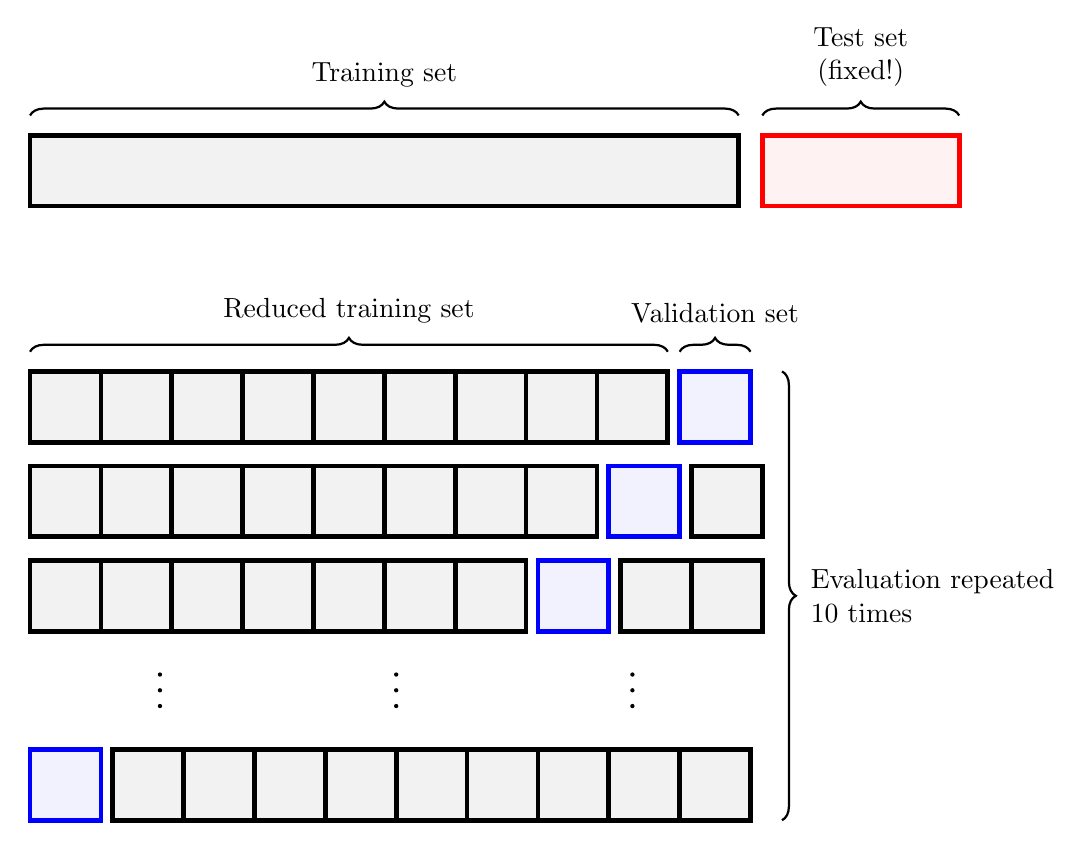
\begin{tikzpicture}
\draw[decorate,decoration={brace,amplitude=5pt},thick] (0,4.15) -- (9,4.15) node[midway,anchor=south,inner sep=0pt,yshift=10pt]{Training set};
\draw[decorate,decoration={brace,amplitude=5pt},thick] (9.3,4.15) -- (11.8,4.15) node[midway,anchor=south,inner sep=0pt,yshift=10pt,align=center]{Test set\\[0pt](fixed!)};
\draw[line width=0.6mm,black,fill=black!05] (0,3) rectangle (9,3.9);
\draw[line width=0.6mm,red,fill=red!05] (9.3,3) rectangle (11.8,3.9);
\draw[decorate,decoration={brace,amplitude=5pt},thick] (0,1.15) -- (8.1,1.15) node[midway,anchor=south,inner sep=0pt,yshift=10pt]{Reduced training set};
\draw[decorate,decoration={brace,amplitude=5pt},thick] (8.25,1.15) -- (9.15,1.15) node[midway,anchor=south,inner sep=0pt,yshift=10pt]{Validation set};
\draw[decorate,decoration={brace,mirror,amplitude=5pt},thick] (9.55,-4.8) -- (9.55,0.9) node[midway,anchor=west,inner sep=0pt,xshift=10pt,align=left]{Evaluation repeated\\[0pt]10 times};
\foreach \y in {-1,0,1} {\fill (1.65,-3.15+\y*0.2) circle (0.0275);}
\foreach \y in {-1,0,1} {\fill (4.65,-3.15+\y*0.2) circle (0.0275);}
\foreach \y in {-1,0,1} {\fill (7.65,-3.15+\y*0.2) circle (0.0275);}
%1
\foreach \i in {0,...,8} {\draw[line width=0.6mm,black,fill=black!05] (0+\i*0.9,0) rectangle (0.9+\i*0.9,0.9);}
\draw[line width=0.6mm,blue,fill=blue!05] (0.15+9*0.9,0) rectangle (0.15+0.9+9*0.9,0.9);
%2
\foreach \i in {0,...,7} {\draw[line width=0.6mm,black,fill=black!05] (0+\i*0.9,-1.2) rectangle (0.9+\i*0.9,0.9-1.2);}
\foreach \i in {9} {\draw[line width=0.6mm,black,fill=black!05] (0.30+\i*0.9,-1.2) rectangle (0.30+0.9+\i*0.9,0.9-1.2);}
\draw[line width=0.6mm,blue,fill=blue!05] (0.15+8*0.9,-1.2) rectangle (0.15+0.9+8*0.9,0.9-1.2);
%3
\foreach \i in {0,...,6} {\draw[line width=0.6mm,black,fill=black!05] (0+\i*0.9,-2.4) rectangle (0.9+\i*0.9,0.9-2.4);}
\foreach \i in {8,9} {\draw[line width=0.6mm,black,fill=black!05] (0.30+\i*0.9,-2.4) rectangle (0.30+0.9+\i*0.9,0.9-2.4);}
\draw[line width=0.6mm,blue,fill=blue!05] (0.15+7*0.9,-2.4) rectangle (0.15+0.9+7*0.9,0.9-2.4);
%10
\foreach \i in {1,...,9} {\draw[line width=0.6mm,black,fill=black!05] (0.15+\i*0.9,-4.8) rectangle (0.15+0.9+\i*0.9,0.9-4.8);}
\draw[line width=0.6mm,blue,fill=blue!05] (0*0.9,-4.8) rectangle (0.9+0*0.9,0.9-4.8);
\end{tikzpicture}
\caption{Schematic representation of the $K$-fold cross-validation.}\label{Cross-validation}
\end{figure}
\begin{figure}[h!t]
\centering
\includegraphics[scale=1.7000]{02_[91-92]_In}
\caption{}\label{02_[91-92]_In}
\end{figure}

Now the decision tree doesn't look as good as it did earlier. In fact, it seems to perform worse than the linear regression model! Notice that cross-validation allows you to get not only an estimate of the performance of your
model, but also a measure of how precise this estimate is (i.e., its standard deviation). The decision tree has a score of approximately \num{71407}, generally $\pm\num{2439}$. You would not have this information if you just used one validation set. But cross-validation comes at the cost of training the model several times, so it is not always possible.

Let's compute the same scores for the linear regression model just to be sure (Fig.~\ref{02_[93]_In}). As we can see from the output, we were right: the decision tree model is overfitting so badly that it performs worse than the linear regression model.
\begin{figure}[h!t]
\centering
\includegraphics[width=\textwidth]{02_[93]_In}
\caption{}\label{02_[93]_In}
\end{figure}

Let's try one last model now: the \jupytercode{RandomForestRegressor}. As we will see in the next sections, random forests work by training many decision trees on random subsets of the features, then averaging out their predictions. Building a model on top of many other models is called \emph{ensemble learning}, and it is often a great way to push machine learning algorithms even further. We will skip most of the code since it is essentially the same as for the other models:

Wow, this is much better: random forests look very promising. However, note that the score on the training set is still much lower than on the validation sets, meaning that the model is still overfitting the training set. Possible solutions for overfitting are to simplify the model, constrain it (i.e., regularize it), or get a lot more training data. Before you dive much deeper into random forests, however, you should try out many other models from various categories of machine learning algorithms (e.g., several support vector machines with different kernels, and possibly a neural network; line \jupytercode{In[98]} of the code), without spending too much time tweaking the hyperparameters. The goal is to shortlist a few (two to five) promising models.
\begin{figure}[h!t]
\centering
\includegraphics[width=\textwidth]{02_[94-96]_In-Out}
\caption{}\label{02_[94-96]_In-Out}
\end{figure}
\subsection{Fine-tune your model}
Let's assume that you now have a shortlist of promising models. You now need to fine-tune them, i.e. to optimize the hyperparameters of the models. Let's look at a few ways you can do that. One option would be to fiddle with the hyperparameters manually, until you find a great combination of hyperparameter values. This would be very tedious work, and you may not have time to explore many combinations.

Instead, you should get Scikit-Learn's \jupytercode{GridSearchCV} to search for you. All you need to do is tell it which hyperparameters you want it to experiment with and what values to try out, and it will use cross-validation to evaluate all the possible combinations of hyperparameter values. For example, the following code (Fig.~\ref{02_[99]_In-Out}) searches for the best combination of hyperparameter values for the \jupytercode{RandomForestRegressor}.
\begin{figure}[h!t]
\centering
\includegraphics[width=\textwidth]{02_[99]_In-Out}
\caption{}\label{02_[99]_In-Out}
\end{figure}

This \jupytercode{param\_grid} tells Scikit-Learn to first evaluate all $3\times4=12$ combinations of \jupytercode{n\_estimators} and \jupytercode{max\_features} hyperparameter values specified in the first \jupytercode{dict} (don't worry about what these hyperparameters mean for now; they will be explained later on), then try all $2\times3=6$ combinations of hyperparameter values in the second \jupytercode{dict}, but this time with the bootstrap hyperparameter set to \jupytercode{False} instead of \jupytercode{True} (which is the default value for this hyperparameter). The grid search will explore $12+6=18$ combinations of \jupytercode{RandomForestRegressor} hyperparameter values, and it will train each model 5 times (since we are using five-fold cross validation). In other words, all in all, there will be $18\times5=90$ rounds of training! It may take quite a long time, but when it is done you can get the best combination of parameters like in Fig.~\ref{02_[100]_In-Out}.
\begin{figure}[h!t]
\centering
\includegraphics[scale=1.7000]{02_[100]_In-Out}
\caption{}\label{02_[100]_In-Out}
\end{figure}

You can also get the best estimator directly (line \jupytercode{In[101]}). And of course the evaluation scores are also available (Fig.~\ref{02_[102]_In}).
\begin{figure}[h!t]
\centering
\includegraphics[width=\textwidth]{02_[102]_In}
\caption{}\label{02_[102]_In}
\end{figure}

In this example, we obtain the best solution by setting the \jupytercode{max\_features} hyperparameter to 8 and the \jupytercode{n\_estimators} hyperparameter to 30. Notice that they are exactly the maximum values in the lists \jupytercode{n\_estimators} and \jupytercode{max\_features}; so this grid search suggests that the algorithm works better with the highest values. This means that if we include other larger values, they are likely to provide even better estimates; but to be sure it would be necessary to check. Anyway, the RMSE score for this combination is \num{49682}, which is slightly better than the score you got earlier using the default hyperparameter values (which was \num{50182}). Congratulations, you have successfully fine-tuned your best model!

The grid search approach is fine when you are exploring relatively few combinations, like in the previous example, but when the hyperparameter search space is large, it is often preferable to use \jupytercode{RandomizedSearchCV} instead. This class can be used in much the same way as the \jupytercode{GridSearchCV} class, but instead of trying out all possible combinations, it evaluates a given number of random combinations by selecting a random value for each hyperparameter at every iteration. An example is given at lines \jupytercode{In[104]}--\jupytercode{In[105]}.
\subsection{Analyze the best models and their errors}
You will often gain good insights on the problem by inspecting the best models. For example, the \jupytercode{RandomForestRegressor} can indicate the relative importance of each attribute for making accurate predictions. Let's display these importance scores next to their corresponding attribute names (Fig.~\ref{02_[107]_In-Out}). These numbers specify how much each of the various attributes affects the price of houses. For example, as we have already anticipated, the \jupytercode{median\_income} is strongly correlated to the prices. With these information, you may want to try dropping some of the less useful features; for instance, apparently only one \jupytercode{ocean\_proximity} category is really useful, so you could try dropping the others.
%You should also look at the specific errors that your system makes, then try to understand why it makes them and what could fix the problem (adding extra features or getting rid of uninformative ones, cleaning up outliers, etc.).
\begin{figure}[h!t]
\centering
\includegraphics[width=\textwidth]{02_[107]_In-Out}
\caption{}\label{02_[107]_In-Out}
\end{figure}
\subsection{Evaluate your system on the test set}
After tweaking your models for a while, you eventually have a system that performs sufficiently well. Now is the time to evaluate the final model on the test set. There is nothing special about this process; just get the predictors and the labels from your test set, run your \jupytercode{full\_pipeline} to transform the data and evaluate the final model on the test set. The machine gives us a root-mean-square error of \num{47730}; so it's comparable to the typical error made experts of houses and is just slightly better than before.

In some cases, such a point estimate of the generalization error will not be quite enough to convince you to launch: what if it is just \SI{0.1}{\percent} better than the model currently in production? You might want to have an idea of how precise this estimate is. For this, you can compute a \SI{95}{\percent} \emph{confidence interval} for the generalization error using \jupytercode{scipy.stats.t.interval}.

In this California housing example, the final performance of the system is not better than the experts' price estimates, which were often off by about \SI{20}{\percent}, but it may still be a good idea to launch it, especially if this frees up some time for the experts so they can work on more interesting and productive tasks.
\section{Training models}
So far we have treated machine learning models and their training algorithms mostly like black boxes. If you went through some of the exercises in the previous sections, you may have been surprised by how much you can get done without knowing anything about what's under the hood: you optimized a regression system, you improved a digit image classifier, and you even built a spam classifier from scratch, all this without knowing how they actually work. Indeed, in many situations you don't really need to know the implementation details.

However, having a good understanding of how things work can help you quickly home in on the appropriate model, the right training algorithm to use, and a good set of hyperparameters for your task. Understanding what's under the hood will also help you debug issues and perform error analysis more efficiently. For the following list of models refer to the notebook \attachfile[icon=CustomPushPin,modified=20210508023432+01'00',size=762869]{Attachments/04_training_linear_models.ipynb}.
\subsection{Linear regression}
First, we will start by looking at the \textbf{linear regression} model, one of the simplest models there is. Generally speaking, a linear model makes a prediction by simply computing a weighted sum of the input features, plus a constant called the \emph{bias term} (also called the intercept term), as shown below:
\begin{equation}\label{LinearRegression}
\widehat{y}=\theta_0+\theta_1x_1+\theta_2x_2+\ldots+\theta_nx_n
\end{equation}
This model is just a linear function of the input features $x_i$, while $\theta_0,\theta_1,\ldots,\theta_n$ are the model's parameters. It is called ``linear'' because the input features enter linearly in the equation, but geometrically speaking equation \eqref{LinearRegression} represents a hyperplane in $n+1$ dimensions\footnote{A hyperplane is a subspace whose dimension is one less than that of its ambient space.}; e.g., for $n=1$ it represents a straight line in 2 dimensions. The quantity $\widehat{y}$ represents the predicted value, and it can be written much more concisely using a vectorized form:
\begin{equation}\label{predictedvalue}
\widehat{y}\equiv h_{\boldtheta}(\mathbf{x})=\boldtheta\cdot\mathbf{x}=\boldtheta^{\mathrm{T}}\mathbf{x}
\end{equation}
In this equation $\boldtheta$ and $\mathbf{x}$ are the model's \emph{parameter vector} and instance's \emph{feature vector}, respectively:
\begin{equation}
\boldtheta=\begin{pmatrix}
\theta_0 \\
\theta_1 \\
\vdots \\
\theta_n
\end{pmatrix}\,,\qquad\quad
\mathbf{x}=\begin{pmatrix}
1 \\
x_1 \\
\vdots \\
x_n
\end{pmatrix}
\end{equation}
while $\boldtheta\cdot\mathbf{x}$ is the standard scalar product of these vectors and $ h_{\boldtheta}$ is the hypothesis function, using the model parameters. Notice that we have set $x_0=1$ in order to reproduce the bias term.

Now, recall that training a model means setting its parameters so that the model best fits the training set. For this purpose, we first need a measure of how well (or poorly) the model fits the training data. At the beginning of Sec.~\ref{sec:Californiahousingprices} we saw that the most common performance measure of a regression model is the root-mean-square error (RMSE):
\begin{equation}\label{RMSE_linear}
\operatorname{RMSE}=\sqrt{\frac{1}{m}\sum_{i=1}^m{\Bigl(\boldtheta^{\mathrm{T}}\mathbf{x}^{(i)}-y^{(i)}\Bigr)}^2}
\end{equation}
Therefore, to train a linear regression model, we need to find the value of $\boldtheta$ that minimizes the RMSE. In practice, it is simpler to minimize the mean squared error (MSE):
\begin{equation}\label{MSE_linear}
\tcbhighmath{\operatorname{MSE}=\frac{1}{m}\sum_{i=1}^m{\Bigl(\boldtheta^{\mathrm{T}}\mathbf{x}^{(i)}-y^{(i)}\Bigr)}^2}
\end{equation}
than the RMSE, and it leads to the same result (because the value that minimizes a function also minimizes its square root). N.B.: written in these forms, equations \eqref{RMSE_linear} and \eqref{MSE_linear} only apply to the linear regression model, since we have already made explicit the functional form of the hypothesis function $h_{\boldtheta}(\mathbf{x})$ as $\boldtheta^{\mathrm{T}}\mathbf{x}$.

To find the value of $\boldtheta$ that minimizes the cost function, it would be sufficient to calculate the derivative of the mean squared error and set the result equal to 0. However, we realize that by introducing the matrix $\mathbf{X}$ of the features values
\begin{equation}
\mathbf{X}=\begin{pmatrix}
{\bigl(\mathbf{x}^{(1)}\bigr)}^{\mathrm{T}}\\
{\bigl(\mathbf{x}^{(2)}\bigr)}^{\mathrm{T}}\\
\vdots\\
{\bigl(\mathbf{x}^{(m)}\bigr)}^{\mathrm{T}}
\end{pmatrix}=\begin{pmatrix}
x_0^{(1)} & x_1^{(1)} & \cdots & x_n^{(1)} \\
x_0^{(2)} & x_1^{(2)} & \cdots & x_n^{(2)} \\
\vdots & \vdots & \ddots & \vdots \\
x_0^{(m)} & x_1^{(m)} & \cdots & x_n^{(m)}
\end{pmatrix}
\end{equation}
this matrix is generally not a square matrix. In fact it is a $m\times(n+1)$ matrix; therefore, if $m\neq n+1$, this matrix is not square. Accordingly, when computing the derivative, the procedure can become a bit tricky. For this reason, we just quote the closed-form solution, i.e. a mathematical equation that gives the result directly, called the \textbf{normal equation} and given by
\begin{equation}
\tcbhighmath{\widehat{\boldtheta}={\bigl(\mathbf{X}^{\mathrm{T}}\mathbf{X}\bigr)}^{-1}\mathbf{X}^{\mathrm{T}}\mathbf{y}}
\end{equation}
So, in this equation $\widehat{\boldtheta}$ is the value of $\boldtheta$ that minimizes the cost function (the error) and $\mathbf{y}$ is the vector of target values:
\begin{equation}
\mathbf{y}=\begin{pmatrix}
y^{(1)} \\
y^{(2)} \\
\vdots \\
y^{(m)}
\end{pmatrix}
\end{equation}
Note that the dimensions of $\widehat{\boldtheta}$ are well defined because the product gives
\begin{equation}
\begin{split}
\widehat{\boldtheta}&={\left(\matrixbg{m\times(n+1)}^{\mathrm{T}}\matrixbg{m\times(n+1)}\right)}^{-1}\matrixbg{m\times(n+1)}^{\mathrm{T}}\matrixbg{m\times1}\\
&={\biggl(\matrixbg{(n+1)\times m}\matrixbg{m\times(n+1)}\biggr)}^{-1}\matrixbg{(n+1)\times m}\matrixbg{m\times1}\\
&=\matrixbg{(n+1)\times(n+1)}^{-1}\matrixbg{(n+1)\times 1}\\
&=\matrixbg{(n+1)\times(n+1)}\matrixbg{(n+1)\times 1}\\
&=\matrixbg{(n+1)\times 1}
\end{split}
\end{equation}
%-------------------------------------------------------------------------------------------------------------------------------------------------------------
%\begin{equation}
%\begin{split}
%\widehat{\boldtheta}&={\left(\matrixbg{m\times(n+1)}^{\mathrm{T}}\matrixbg{m\times(n+1)}\right)}^{-1}\matrixbg{m\times(n+1)}^{\mathrm{T}}\matrixbg{m\times1}\\
%&={\biggl(\matrixbg{(n+1)\times m}\matrixbg{m\times(n+1)}\biggr)}^{-1}\matrixbg{(n+1)\times m}\matrixbg{m\times1}\\
%&=\matrixbg{(n+1)\times(n+1)}^{-1}\matrixbg{(n+1)\times m}\matrixbg{m\times1}\\
%&=\matrixbg{(n+1)\times(n+1)}\matrixbg{(n+1)\times m}\matrixbg{m\times1}\\
%&=\matrixbg{(n+1)\times m}\matrixbg{m\times1}\\
%&=\matrixbg{(n+1)\times 1}
%\end{split}
%\end{equation}
%-------------------------------------------------------------------------------------------------------------------------------------------------------------
%{\left(\matrixframe{1.2}{1.8}_{m\times(n+1)}^{\mathrm{T}}\matrixframe{1.2}{1.8}_{m\times(n+1)}\right)}^{-1}\matrixframe{1.2}{1.8}_{m\times(n+1)}^{\mathrm{T}}\matrixframe{1.8}{0.6}_{m\times1}\\
%&={\left(\matrixframe{1.8}{1.2}_{(n+1)\times m}\matrixframe{1.2}{1.8}_{m\times(n+1)}\right)}^{-1}\matrixframe{1.8}{1.2}_{(n+1)\times m}\matrixframe{1.8}{0.6}_{m\times1}\\
%&={\left(\matrixframe{1.8}{1.2}_{(n+1)\times m}\matrixframe{1.2}{1.8}_{m\times(n+1)}\right)}^{-1}\matrixframe{1.8}{1.2}_{(n+1)\times m}\matrixframe{1.8}{0.6}_{m\times1}\\
%-------------------------------------------------------------------------------------------------------------------------------------------------------------
%{\left(\matrixframe{2.25}{1.5}{(n+1)\times m}\matrixframe{1.5}{2.25}{m\times(n+1)}\right)}^{-1}\matrixframe{2.25}{1.5}{(n+1)\times m}\matrixframe{0.75}{2.25}{m\times 1}\\
%-------------------------------------------------------------------------------------------------------------------------------------------------------------

Let's generate some linear-looking data to test this equation; this type of data are sometimes called ``mock data'' because they are simulated samples that mimic the behavior of real objects in controlled ways, most often exploited as part of a testing initiative. To do this, we have first generated 100 random numbers $x_i$ uniformly distributed between 0 and 2, and then we have created the corresponding $y_i$ according to the function $y_i=4+3x_i+\text{Gaussian noise}$ (Fig.~\ref{04_[2]_In}).
\begin{figure}[h!t]
\centering
\includegraphics[scale=1.2820]{04_[2]_In}
\caption{}\label{04_[2]_In}
\end{figure}

Now let's compute $\widehat{\boldtheta}$ using the normal equation (Fig.~\ref{04_[4-5]_In-Out}). Looking at what the equation found, we would have hoped for $\theta_0=4$ and $\theta_1=3$ instead of $\theta_0=4.215$ and $\theta_1=2.770$. Close enough, but the noise made it impossible to recover the exact parameters of the original function.
\begin{figure}[h!t]
\centering
\includegraphics[scale=1.2820]{04_[4-5]_In-Out}
\caption{}\label{04_[4-5]_In-Out}
\end{figure}

Anyway, now we can make predictions using $\widehat{y}=\widehat{\boldtheta}\cdot\mathbf{x}=\widehat{\boldtheta}^{\mathrm{T}}\mathbf{x}$, i.e. equation \eqref{predictedvalue}. In Figure~\ref{04_[8]_In} are shown the initial data (blue points) and the best linear model optimized with the parameters dictated by $\widehat{\boldtheta}$ (red line).
\begin{figure}[h!t]
\centering
\includegraphics[scale=0.65]{04_[8]_In}
\caption{}\label{04_[8]_In}
\end{figure}

In the previous lines we computed the best fit ``manually'', directly exploiting the expression of the normal equation. But in general, performing linear regression is much more simple using Scikit-Learn because it already has an implemented function dedicated to it: \jupytercode{scipy.linalg.lstsq()} (Fig.~\ref{04_[9]_In-Out}). However, the normal equation expects to invert a matrix, and this can be particularly delicate or unstable for a variety of reasons. Therefore, this function actually computes $\widehat{\boldtheta}=\mathbf{X}^+\mathbf{y}$, where $\mathbf{X}^+$ is the Moore--Penrose inverse or \emph{pseudoinverse} of $\mathbf{X}$ ($\mathbf{X}^+$ is a specific notation; it does not mean hermitian conjugate). The pseudoinverse itself is computed using a standard matrix factorization technique called \emph{singular value decomposition} (SVD) that can decompose the training set matrix $\mathbf{X}$ into the matrix multiplication of three matrices: $\mathbf{X}=\mathbf{U}\boldsymbol{\Sigma}\mathbf{V}^{\mathrm{T}}$ (see \jupytercode{numpy.linalg.svd()}). The pseudoinverse is computed as $\mathbf{X}^+=\mathbf{V}\boldsymbol{\Sigma}^+\mathbf{U}^{\mathrm{T}}$. To compute the matrix $\boldsymbol{\Sigma}^+$, the algorithm takes $\boldsymbol{\Sigma}$ and sets to zero all values smaller than a tiny threshold value, then it replaces all the nonzero values with their reciprocals, and finally it transposes the resulting matrix. This approach is more efficient than computing the normal equation, plus it handles edge cases nicely: indeed, the normal equation may not work if the matrix $\mathbf{X}^{\mathrm{T}}\mathbf{X}$ is not invertible (i.e., singular), such as if $m<n$ or if some features are redundant, but the pseudoinverse is always defined. naturally, for invertible matrices the pseudoinverse equals the usual inverse.
\begin{figure}[h!t]
\centering
\includegraphics[scale=1.385]{04_[9]_In-Out}
\caption{}\label{04_[9]_In-Out}
\end{figure}

The normal equation computes the inverse of $\mathbf{X}^{\mathrm{T}}\mathbf{X}$, which is an $(n+1)\times(n+1)$ matrix, where $n$ is the number of features. The computational complexity of inverting such a matrix is typically about $O(n^{2.4})$ to $O(n^{3})$, depending on the implementation. In other words, if you double the number of features, you multiply the computation time by roughly $2^{2.4}\simeq5.3$ to $2^{3}=8$. Instead, the SVD approach used by Scikit-Learn's \jupytercode{LinearRegression} class is about $O(n^{2})$. If you double the number of features, you multiply the computation time by roughly 4.

Keep in mind that both the normal equation and the SVD approach get very slow when the number of features grows large (e.g., \num{100000}). On the positive side, both are linear with regard to the number of instances in the training set, $O(m)$, so they handle large training sets efficiently, provided they can fit in memory.

Now we will look at a very different way to train a Linear Regression model, which is better suited for cases where there are a large number of features or too many training instances to fit in memory.
\subsection{Gradient descent}\label{subsec:Gradient_descent}
\textbf{Gradient descent} is a generic optimization algorithm capable of finding optimal solutions to a wide range of problems (we have already seen it when we spoke about neutral networks). The general idea of gradient descent is to tweak parameters iteratively in order to minimize a cost function (Fig.~\ref{GradientDescent}). This technique measures the local gradient of the error function with regard to the parameter vector $\boldtheta$, and it goes in the direction of descending gradient. Once the gradient is zero, we have reached a minimum! Concretely, we start by filling $\boldtheta$ with random values (this is called random initialization). Then you improve it gradually, taking one baby step at a time, each step attempting to decrease the cost function (e.g., the MSE), until the algorithm converges to a minimum:
\begin{equation}\label{eqn:GradientDescent}
\tcbhighmath{\boldtheta^{\text{next}}=\boldtheta-\eta\boldsymbol{\nabla}_{\boldtheta}\operatorname{MSE}}
\end{equation}
(computing $\boldsymbol{\nabla}_{\boldtheta}\operatorname{MSE}$ leads to $\frac{2}{m}\mathbf{X}^{\mathrm{T}}(\mathbf{X}\boldtheta-\mathbf{y})$).
\begin{figure}[h!t]
\centering
\includegraphics[scale=0.265]{Gradient Descent}
\caption{}\label{GradientDescent}
\end{figure}

An important parameter in gradient descent is the size of the steps, determined by the \emph{learning rate} hyperparameter $\eta$. If the learning rate is too small, then the algorithm will have to go through many iterations to converge, which will take a long time. On the other hand, if the learning rate is too high, you might jump across the valley and end up on the other side, possibly even higher up than you were before. This might make the algorithm diverge, with larger and larger values, failing to find a good solution. Figure~\ref{04_[17]_In} shows the first 10 steps of gradient descent using three different learning rates (the dashed line represents the starting point). On the left, the learning rate is too low: the algorithm will eventually reach the solution, but it will take a long time. In the middle, the learning rate looks pretty good: in just a few iterations, it has already converged to the solution. On the right, the learning rate is too high: the algorithm diverges, jumping all over the place and actually getting further and further away from the solution at every step.
\begin{figure}[h!t]
\centering
\includegraphics[width=\textwidth]{04_[17]_In}
\caption{Gradient descent with various learning rates.}\label{04_[17]_In}
\end{figure}

Finally, not all cost functions look like nice, regular bowls. There may be holes, ridges, plateaus, and all sorts of irregular terrains, making convergence to the minimum difficult. Figure~\ref{GradientDescentPitfalls} shows the two main challenges with gradient descent. If the random initialization starts the algorithm on the left, then it will converge to a \emph{local minimum}, which is not as good as the \emph{global minimum}. If it starts on the right, then it will take a very long time to cross the plateau. And if you stop too early, you will never reach the global minimum.
\begin{figure}[h!t]
\centering
\includegraphics[scale=0.265]{Gradient Descent Pitfalls}
\caption{}\label{GradientDescentPitfalls}
\end{figure}

Fortunately, the MSE cost function for a linear regression model happens to be a \emph{convex function}, which means that if you pick any two points on the curve, the line segment joining them never crosses the curve. This implies that there are \emph{no local minima, just one global minimum}. It is also a continuous function with a slope that never changes abruptly. These two facts have a great consequence: gradient descent is guaranteed to approach arbitrarily close the global minimum (if you wait long enough and if the learning rate is not too high).

In fact, the cost function has the shape of a bowl, but it can be an elongated bowl if the features have very different scales. Figure~\ref{GradientDescentScale} shows gradient descent on a training set where features 1 and 2 have the same scale (on the left), and on a training set where feature 1 has much smaller values than feature 2 (on the right). As you can see, on the left the gradient descent algorithm goes straight toward the minimum, thereby reaching it quickly, whereas on the right it first goes in a direction almost orthogonal to the direction of the global minimum, and it ends with a long march down an almost flat valley. It will eventually reach the minimum, but it will take a long time. Therefore, when using gradient descent, you should \emph{ensure that all features have a similar scale}, or else it will take much longer to converge.
\begin{figure}[h!t]
\centering
\includegraphics[scale=0.365]{Gradient Descent Scale}
\caption{Gradient Descent with (left) and without (right) feature scaling.}\label{GradientDescentScale}
\end{figure}
\subsubsection{Stochastic gradient descent}
Notice that formula \eqref{eqn:GradientDescent} involves calculations over the full training set $\mathbf{X}$, at each gradient descent step! This is why the algorithm is called \textbf{batch gradient descent}: it uses the whole batch of training data at every step (actually, full gradient descent would probably be a better name). As a result it is terribly slow on very large training sets.

A possible solution is \textbf{stochastic gradient descent}, which picks a random instance in the training set at every step and computes the gradients based only on that single instance. Obviously, working on a single instance at a time makes the algorithm much faster because it has very little data to manipulate at every iteration. It also makes it possible to train on huge training sets, since only one instance needs to be in memory at each iteration.

On the other hand, due to its stochastic (i.e., random) nature, this algorithm is much less regular than batch gradient descent: instead of gently decreasing until it reaches the minimum, the cost function will bounce up and down, decreasing only on average. Over time it will end up very close to the minimum, but once it gets there it will continue to bounce around, never settling down (see Fig.~\ref{StochasticGradientDescent}). So once the algorithm stops, the final parameter values are good, but not optimal.
\begin{figure}[h!t]
\centering
\includegraphics[scale=0.2]{Stochastic Gradient Descent}
\caption{}\label{StochasticGradientDescent}
\end{figure}

Moreover, when the cost function is very irregular (as in Figure~\ref{GradientDescentPitfalls}), this can actually help the algorithm jump out of local minima, so stochastic gradient descent has a better chance of finding the global minimum than batch gradient descent does.

Therefore, randomness is good to escape from local optima, but bad because it means that the algorithm can never settle at the minimum. One solution to this dilemma is to gradually reduce the learning rate, a process akin to \emph{simulated annealing}. The steps start out large (which helps make quick progress and escape local minima), then get smaller and smaller, allowing the algorithm to settle at the global minimum. The function that determines the learning rate at each iteration is called the \emph{learning schedule}. If the learning rate is reduced too quickly, you may get stuck in a local minimum, or even end up frozen halfway to the minimum. If the learning rate is reduced too slowly, you may jump around the minimum for a long time and end up with a suboptimal solution if you halt training too early. The code in Fig.~\ref{04_[19]_In} implements stochastic gradient descent using a simple learning schedule:
\begin{equation}
\text{Learning schedule}=\frac{t_0}{t+t_1}
\end{equation}
where $t_0$ and $t_1$ are hyperparameters of the model, while $t$ indicates the time. By convention we iterate by rounds of $m$ iterations; each round is called an \emph{epoch}. While the batch gradient descent code iterated \num{1000} times through the whole training set, this code goes through the training set only 50 times and reaches a pretty good solution.
\begin{figure}[h!t]
\centering
\includegraphics[width=\textwidth]{04_[19]_In}
\caption{}\label{04_[19]_In}
\end{figure}
\subsubsection{Mini-batch gradient descent}
The last gradient descent algorithm we will look at is called \textbf{mini-batch gradient descent}. It is simple to understand once you know batch and stochastic gradient descent: at each step, instead of computing the gradients based on the full training set (as in batch GD) or based on just one instance (as in stochastic GD), mini-batch GD computes the gradients on small random sets of instances called \emph{mini-batches}.

The algorithm's progress in parameter space is less erratic than with stochastic GD, especially with fairly large mini-batches. As a result, mini-batch GD will end up walking around a bit closer to the minimum than stochastic GD. But it may be harder for it to escape from local minima (in the case of problems that suffer from local minima, unlike linear regression). Figure~\ref{04_[26]_In} shows the paths taken by the three gradient descent algorithms in parameter space during training. They all end up near the minimum, but batch GD's path actually stops at the minimum, while both stochastic GD and mini-batch GD continue to walk around.
%However, don't forget that batch GD takes a lot of time to take each step, and stochastic GD and mini-batch GD would also reach the minimum if you used a good learning schedule.
\begin{figure}[h!t]
\centering
\includegraphics[scale=0.65]{04_[26]_In}
\caption{}\label{04_[26]_In}
\end{figure}
\subsection{Polynomial regression}\label{sec:Polynomial_regression}
What if your data is more complex than a straight line? Surprisingly, you can still use a linear model to fit nonlinear data. A simple way to do this is to add powers of each feature as new features, then train a linear model on this extended set of features. This technique is called \textbf{polynomial regression}. For instance, suppose we have just one feature and many instances; if we have expect a quadratic relation between $x$ and $y$:
\begin{equation}\label{PolynomialRegression}
\widehat{y}=\theta_0+\theta_1x_1+\theta_2x_1^2
\end{equation}
then we take the initial sample
\begin{equation}
\Bigl\{x_1^{(1)},\ldots,x_1^{(m)}\Bigr\}
\end{equation}
and we replace it with the extended
%\begin{equation}
%\Bigl\{x_1^{(1)},{\bigl(x_1^{(1)}\bigr)}^2,\ldots,x_1^{(m)},{\bigl(x_1^{(m)}\bigr)}^2\Bigr\}
%\end{equation}
\begin{equation}
\begin{matrix}
\Bigl\{x_1^{(1)},{\bigl(x_1^{(1)}\bigr)}^2,\ldots,x_1^{(m)},{\bigl(x_1^{(m)}\bigr)}^2\Bigr\} \vspace{4pt}\\
\Big\downarrow \vspace{4pt}\\
\Bigl\{\overline{x}_1^{(1)},\overline{x}_2^{(1)},\ldots,\overline{x}_1^{(m)},\overline{x}_2^{(m)}\Bigr\}
\end{matrix}
\end{equation}
such that we can apply a linear regression model of the type
\begin{equation}
\widehat{y}=\theta_0+\theta_1\overline{x}_1+\theta_2\overline{x}_2
\end{equation}
with two features instead of just one.

Let's look at an example (Figs.~\ref{04_[28-32]_In-Out} and \ref{04_[33]_In}). First, let's generate some nonlinear data, based on a simple quadratic equation (plus some noise). Clearly, a straight line will never fit this data properly. So let's use Scikit-Learn's \jupytercode{PolynomialFeatures} class to transform our training data, adding the square (second-degree polynomial) of each feature in the training set as a new feature (in this case there is just one feature\footnote{Note that when there are multiple features, polynomial regression is capable of finding relationships between features (which is something a plain linear regression model cannot do). This is made possible by the fact that \jupytercode[0.82]{PolynomialFeatures} also adds all combinations of features up to the given degree. E.g. combinations like $x_1x_2$.}). \jupytercode{X\_poly} now contains the original feature of \jupytercode{X} plus the square of this feature. Now you can fit a \jupytercode{LinearRegression} model to this extended training data. The result are not bad: the model estimates $\widehat{y}=0.56x_1^2+0.93x_1+1.78$ when in fact the original function was $\widehat{y}=0.5x_1^2+1.0x_1+2.0+\text{Gaussian noise}$.
\begin{figure}[h!t]
\centering
\includegraphics[scale=1.2820]{04_[28-32]_In-Out}
\caption{}\label{04_[28-32]_In-Out}
\end{figure}
\begin{figure}[h!t]
\centering
\includegraphics[scale=0.65]{04_[33]_In}
\caption{Polynomial regression model predictions (\jupytercode[0.913]{In[33]}).}\label{04_[33]_In}
\end{figure}

Notice that this procedure can be done only for a certain class of functions, like polynomials. For example, if we modeled with a function like $e^{ax}/x$ there would be no possibility of being able to reduce it to a linear model.
\subsection{Learning curves}
If you perform high-degree polynomial regression, you will likely fit the training data much better than with plain Linear Regression. For example, Figure~\ref{04_[34]_In} applies a $300$-degree polynomial model to the preceding training data, and compares the result with a pure linear model and a quadratic model (second-degree polynomial). Notice how the 300-degree polynomial model wiggles around to get as close as possible to the training instances. This high-degree polynomial regression model is severely overfitting the training data, while the linear model is underfitting it. The model that will generalize best in this case is the quadratic model, which makes sense because the data was generated using a quadratic model. But in general you won't know what function generated the data, so how can you decide how complex your model should be? How can you tell that your model is overfitting or underfitting the data?
\begin{figure}[h!t]
\centering
\includegraphics[scale=0.65]{04_[34]_In}
\caption{}\label{04_[34]_In}
\end{figure}

In Section~\ref{sec:cross-validation} we used cross-validation to get an estimate of a model's generalization performance. If a model performs well on the training data but generalizes poorly according to the cross-validation metrics, then your model is overfitting. If it performs poorly on both, then it is underfitting. This is one way to tell when a model is too simple or too complex.

Another way to tell is to look at the \textbf{learning curves}: these are plots of the model's performance on the training set and the validation set as a function of the training set size (or the training iteration). To generate the plots, train the model several times on different sized subsets of the training set.

Let’s look at the learning curves of the plain linear regression model (a straight line; see Fig.~\ref{04_[36]_In}). This model that's underfitting deserves a bit of explanation. First, let's look at the performance on the training data: when there are just one or two instances in the training set, the model can fit them perfectly, which is why the curve starts at zero (one, and only one, line passes through two points). But as new instances are added to the training set, it becomes impossible for the model to fit the training data perfectly with a straight line, both because the data are noisy and because it is not linear at all. So the error on the training data goes up until it reaches a plateau, at which point adding new instances to the training set doesn't make the average error much better or worse. Now let's look at the performance of the model on the validation data. When the model is trained on very few training instances, it is incapable of generalizing properly, which is why the validation error is initially quite big. Then, as the model is shown more training examples, it learns, and thus the validation error slowly goes down. However, once again a straight line cannot do a good job modeling the data, so the error ends up at a plateau, very close to the other curve. These learning curves are typical of a model that's underfitting. Both curves have reached a plateau; they are close and fairly high.
\begin{figure}[h!t]
\centering
\includegraphics[scale=0.65]{04_[36]_In}
\caption{Learning curves for the linear regression model.}\label{04_[36]_In}
\end{figure}

Now let's look at the learning curves of a 10-th-degree polynomial model on the same data (Fig.~\ref{04_[37]_In}). These learning curves look a bit like the previous ones, but there are two very important differences:
\begin{itemize}
\item The error on the training data is much lower than with the linear regression model.
\item There is a gap between the curves. This means that the model performs significantly better on the training data than on the validation data, which is the hallmark of an overfitting model. If you used a much larger training set, however, the two curves would continue to get closer.
\end{itemize}
\begin{figure}[h!t]
\centering
\includegraphics[scale=0.65]{04_[37]_In}
\caption{Learning curves for the 10-th-degree polynomial model.}\label{04_[37]_In}
\end{figure}
\subsubsection{On the nature of errors}
An important theoretical result of statistics and machine learning is the fact that a model's generalization error can be expressed as the sum of three very different errors:
\begin{description}
\item[Bias] This part of the generalization error is due to wrong assumptions, such as assuming that the data are linear when it is actually quadratic. A high-bias model is most likely to underfit the training data.
\item[Variance] This part is due to the model's excessive sensitivity to small variations in the training data. A model with many degrees of freedom (such as a high-degree polynomial model) is likely to have high variance and thus overfit the training data.
\item[Irreducible error]
This part is due to the noisiness of the data itself. The only way to reduce this part of the error is to clean up the data (e.g., fix the data sources, such as broken sensors, or detect and remove outliers).
\end{description}
Increasing a model's complexity will typically increase its variance and reduce its bias. Conversely, reducing a model's complexity increases its bias and reduces its variance. This is why it is called a trade-off.
\subsection{Regularized linear models}
As we saw in Section~\ref{sec:Testing_and_validating}, a good way to reduce overfitting is to regularize the model (i.e., to constrain it): the fewer degrees of freedom it has, the harder it will be for it to overfit the data. A simple way to regularize a polynomial model is to reduce the number of polynomial degrees. For a linear model, regularization is typically achieved by constraining the weights of the model.
\subsubsection{Ridge regression}
\textbf{Ridge regression} (also called \emph{Tikhonov regularization}) is a regularized version of linear regression based on a regularization term equal to $\alpha\frac{1}{2}\sum_{i=1}^n\theta_i^2$ added to the cost function:
\begin{equation}
\tcbhighmath{J(\boldtheta)=\text{MSE}+\alpha\frac{1}{2}\sum_{i=1}^n\theta_i^2}
\end{equation}
Note that the bias term $\theta_0$ is not regularized (the sum starts at $i=1$, not $0$). Anyway, ridge regression forces the learning algorithm to not only fit the data but also keep the model weights as small as possible. Note that the regularization term should only be added to the cost function during training. Once the model is trained, you want to use the unregularized performance measure to evaluate the model's performance.

The hyperparameter $\alpha$ controls how much you want to regularize the model. If $\alpha=0$, then ridge regression is just linear regression. If $\alpha$ is very large, then all weights end up very close to zero and the result is a flat line going through the data's mean.

Figure~\ref{04_[41]_In} shows several ridge models trained on some linear data using different $\alpha$ values. On the left, plain ridge models are used, leading to linear predictions. On the right, the data is first expanded using \jupytercode{PolynomialFeatures(degree=10)}, then it is scaled using a \jupytercode{StandardScaler}, and finally the ridge models are applied to the resulting features: this is polynomial regression with ridge regularization. Note how increasing $\alpha$ leads to flatter (i.e., less oscillatory, more reasonable) predictions, thus reducing the model's variance but increasing its bias.
\begin{figure}[h!t]
\centering
\includegraphics[scale=0.65]{04_[41]_In}
\caption{}\label{04_[41]_In}
\end{figure}
\subsubsection{Lasso regression}
Least absolute shrinkage and selection operator regression, usually simply called \textbf{Lasso regression} is another regularized version of linear regression: just like ridge regression, it adds a regularization term to the cost function, but it uses the $\ell_1$ norm of the weight vector instead of half the square of the $\ell_2$ norm\footnote{Remember that the $\ell_p$ norm of a vector $\mathbf{x}=(x_1,\ldots,x_n)$ is defined as
\begin{equation}
\|\mathbf{x}\|_{\ell_p}\coloneqq{\left(\sum_{i=1}^n{\lvert x_i\rvert}^p\right)}^{1/p}
\end{equation}}:
\begin{equation}
\tcbhighmath{J(\boldtheta)=\text{MSE}+\alpha\sum_{i=1}^n\lvert\theta_i\rvert}
\end{equation}
Figure~\ref{04_[43]_In} shows the same thing as Figure~\ref{04_[41]_In} but replaces ridge models with lasso models and uses smaller $\alpha$ values.
\begin{figure}[h!t]
\centering
\includegraphics[scale=0.65]{04_[43]_In}
\caption{}\label{04_[43]_In}
\end{figure}

An important characteristic of lasso regression is that it tends to eliminate the weights of the least important features (i.e., set them to zero). For example, the dashed line in the right-hand plot in Figure~\ref{04_[43]_In} (with $\alpha=10^{-7}$) looks quadratic, almost linear: all the weights for the high-degree polynomial features are equal to zero. In other words, lasso regression automatically performs feature selection and outputs a \emph{sparse model} (i.e., with few nonzero feature weights).
%It doesn't look quadratic, anyway...
%effective in reducing the error: small values that should be 0
\subsubsection{Early stopping}
very different way to regularize iterative learning algorithms such as gradient descent is to stop training as soon as the validation error reaches a minimum. This is called \textbf{early stopping}. Figure~\ref{04_[48]_In} shows a complex model (in this case, a high-degree polynomial regression model) being trained with batch gradient descent. As the epochs go by the algorithm learns, and its prediction error (RMSE) on the training set goes down, along with its prediction error on the validation set. After a while though, the validation error stops decreasing and starts to go back up. This indicates that the model has started to overfit the training data. With early stopping you just stop training as soon as the validation error reaches the minimum.
%It is such a simple and efficient regularization technique that Geoffrey Hinton called it a “beautiful free lunch.”
\begin{figure}[h!t]
\centering
\includegraphics[scale=0.65]{04_[48]_In}
\caption{}\label{04_[48]_In}
\end{figure}
\subsection{Logistic regression}
As we discussed in Section~\ref{sec:Introduction_to_machine_learning}, some regression algorithms can be used for classification (and vice versa). \textbf{Logistic regression} is commonly used to estimate the probability that an instance belongs to a particular class (e.g., what is the probability that this email is spam?). If the estimated probability is greater than \SI{50}{\percent}, then the model predicts that the instance belongs to that class (called the \emph{positive class}, labeled ``1''), and otherwise it predicts that it does not (i.e., it belongs to the \emph{negative class}, labeled ``0''). This makes it a binary classifier.
\subsubsection{Estimating probabilities}
So how does logistic regression work? Just like a linear regression model, a logistic regression model computes a weighted sum of the input features (plus a bias term), but instead of outputting the result directly like the linear regression model does, it outputs the \emph{logistic} of this result
\begin{equation}
\widehat{p}=\sigma(\mathbf{x}^{\mathrm{T}}\boldtheta)%=h_{\boldtheta}(\mathbf{x})
\end{equation}
where
\begin{equation}
\sigma(t)=\frac{1}{1+e^{-t}}
\end{equation}
Here $\sigma$ constitutes the so-called logistic, which is a sigmoidal function (i.e., S-shaped) that outputs a number between 0 and 1 (see Fig.~\ref{04_[53]_In}). The logistic function gives a measure of the \emph{probability} for a specific outcome, and not the exact prediction of the model. Therefore, in order to compute a determined output we need a rule to ``convert'' the logistic function into a step function. So, once the logistic regression model has estimated the probability $\widehat{p}=\sigma(\mathbf{x}^{\mathrm{T}}\boldtheta)$ that an instance $\mathbf{x}$ belongs to the positive class, it can make its prediction $\widehat{y}$ easily as
\begin{equation}
\widehat{y}=\begin{cases}
0\,,&\text{if $\widehat{p}<0.5$}\\
1\,,&\text{if $\widehat{p}\geq0.5$}
\end{cases}
\end{equation}
Notice that $\sigma(t)<0.5$ when $t<0$, and $\sigma(t)\geq0.5$ when $t\geq0$, so a logistic regression model predicts $1$ if $\mathbf{x}^{\mathrm{T}}\boldtheta$ is positive and 0 if it is negative: $\widehat{y}=\Theta(\mathbf{x}^{\mathrm{T}}\boldtheta)$.
\begin{figure}[h!t]
\centering
\includegraphics[scale=0.65]{04_[53]_In}
\caption{}\label{04_[53]_In}
\end{figure}

Note the close similarity between logistic regression and stochastic neural networks (Sec.~\ref{sec:Stochasticneurons}). Also in that case we were used to adopt a deterministic law for the description of the neuron response (sign), but then we introduced a stochastic law based essentially on a Fermi--Dirac distribution. There, the connection between deterministic and stochastic was based on the dependence on a pseudo-temperature, in such a way that for $T\rightarrow0$ we would lead back to the deterministic case.
%This idea is then taken up again in the case of the simple perceptron
\subsubsection{Training and cost function}\label{subsubsec:Training_and_cost_function}
Now you know how a logistic regression model estimates probabilities and makes predictions. But how is it trained? The objective of training is to set the parameter vector $\boldtheta$ so that the model estimates high probabilities for positive instances ($y=1$) and low probabilities for negative instances ($y=0$), i.e. in order to make the smallest possible errors in the classification task. This idea is captured by the \emph{cost function} for a single training instance~$\mathbf{x}$:
\begin{equation}
c(\boldtheta)=\begin{cases}
-\ln{\widehat{p}}\,,&\text{if $y=1$}\\
-\ln{(1-\widehat{p})}\,,&\text{if $y=0$}
\end{cases}
\end{equation}
which measures how far we are from what we want to obtain\footnote{It is quite common to use logarithm functions in logistic tasks.}. This cost function makes sense because $-\ln{\widehat{p}}$ grows very large when $\widehat{p}$ approaches 0, so the cost will be large if the model estimates a probability close to 0 for a positive instance ($y=1$), and it will also be very large if the model estimates a probability close to 1 for a negative instance ($y=0$). On the other hand, $-\ln{\widehat{p}}$ is close to 0 when $\widehat{p}$ is close to 1, so the cost will be close to 0 if the estimated probability is close to 0 for a negative instance or close to 1 for a positive instance, which is precisely what we want.

The cost function over the whole training set is the average cost over all training instances:
\begin{equation}\label{log_loss}
\tcbhighmath{J(\boldtheta)=-\frac{1}{m}\sum_{i=1}^m\Bigl[y^{(i)}\ln{\widehat{p}^{(i)}}+\bigl(1-y^{(i)}\bigr)\ln{\bigl(1-\widehat{p}^{(i)}\bigr)}\Bigr]}
\end{equation}
In fact, if $y^{(i)}=1$ the second term vanishes and the cost for that specific positive instance is $-\ln{\widehat{p}^{(i)}}$, while if $y^{(i)}=0$ it is the first term to cancel itself out and the cost for that specific negative instance is $\ln{\bigl(1-\widehat{p}^{(i)}\bigr)}$. Here we have written the global cost in a single expression, which is usually called the \emph{log loss}. The bad news is that there is no known closed-form equation to compute the value of $\boldtheta$ that minimizes this cost function; in other words, there is no equivalent of the normal equation. However, the good news is that this cost function is convex, so gradient descent\footnote{$\boldsymbol{\nabla}J(\boldtheta)=\frac{1}{m}\mathbf{X}^{\mathrm{T}}(\boldsigma-\mathbf{y})$, with $\boldsigma^{(i)}=\sigma(\boldtheta^{\mathrm{T}}\mathbf{x}^{(i)})$.} (or any other optimization algorithm) is guaranteed to find the global minimum (if the learning rate is not too large and you wait long enough).
\subsubsection{Decision boundaries}
Let's use the Iris dataset to illustrate logistic regression, trying to understand if a certain flower belongs to a specific class. This is a famous dataset that contains the sepal and petal length and width of 150 iris flowers of three different species: \emph{Iris setosa}, \emph{Iris versicolor} and \emph{Iris virginica} (see Figure~\ref{Iris}).
\begin{figure}[h!t]
\centering
\includegraphics[scale=0.25]{Iris}
\caption{}\label{Iris}
\end{figure}

Let's try to build a classifier to detect the \emph{Iris virginica} type based only on the petal width feature. First let's load the data, and then let's train a logistic regression model with the Scikit-Learn's \jupytercode{LogisticRegression()}. Let's look at the model's estimated probabilities for flowers with petal widths varying from \SI{0}{\centi\meter} to \SI{3}{\centi\meter} (Figure~\ref{04_[59]_In}). The petal width of \emph{Iris virginica} flowers (represented by triangles) ranges from \SI{1.4}{\centi\meter} to \SI{2.5}{\centi\meter}, while the other iris flowers (represented by squares) generally have a smaller petal width, ranging from \SI{0.1}{\centi\meter} to \SI{1.8}{\centi\meter}. Notice that there is a bit of overlap. Above about \SI{2}{\centi\meter} the classifier is highly confident that the flower is an \emph{Iris virginica} (it outputs a high probability for that class), while below \SI{1}{\centi\meter} it is highly confident that it is not an \emph{Iris virginica} (high probability for the ``Not \emph{Iris virginica}'' class). In between these extremes, the classifier is unsure. However, if you ask it to predict the class, it will return whichever class is the most likely. Therefore, there is a \emph{decision boundary} at around \SI{1.6}{\centi\meter} where both probabilities are equal to \SI{50}{\percent}: if the petal width is higher than \SI{1.6}{\centi\meter}, the classifier will predict that the flower is an \emph{Iris virginica}, and otherwise it will predict that it is not (even if it is not very confident).
\begin{figure}[h!t]
\centering
\includegraphics[scale=0.65]{04_[59]_In}
\caption{}\label{04_[59]_In}
\end{figure}

Figure~\ref{04_[62]_In} shows the same dataset, but this time displaying two features: petal width and length. Once trained, the logistic regression classifier can, based on these two features, estimate the probability that a new flower is an \emph{Iris virginica}. The dashed line represents the points where the model estimates a \SI{50}{\percent} probability: this is the model's decision boundary. Note that it is a linear boundary. Each parallel line represents the points where the model outputs a specific probability, from \SI{15}{\percent} (bottom left) to \SI{90}{\percent} (top right). All the flowers beyond the top-right line have an over \SI{90}{\percent} chance of
being \emph{Iris virginica}, according to the model.
\begin{figure}[h!t]
\centering
\includegraphics[width=\textwidth]{04_[62]_In}
\caption{}\label{04_[62]_In}
\end{figure}
%Also in perceptron we were trying to separate the two classes with a line
%here we are using two neurons...
\subsubsection{Softmax regression}\label{subsubsec:Softmax_regression}
Whereas binary classifiers distinguish between two classes, \emph{multiclass classifiers} (also called multinomial classifiers) can distinguish between more than two classes. The logistic regression model can be generalized to support multiple classes directly, without having to train and combine multiple binary classifiers. This is called \emph{softmax regression}, or \emph{multinomial logistic regression}. The idea is simple: when given an instance $\mathbf{x}$, the softmax regression model first computes a score $s_k(\mathbf{x})$ for each class $k$, then estimates the probability of each class by applying the softmax function (also called the normalized exponential) to the scores.

The equation to compute $s_k(\mathbf{x})$ should look familiar, as it is just like the equation for linear regression prediction
\begin{equation}
s_k(\mathbf{x})=\mathbf{x}^{\mathrm{T}}\boldtheta^{(k)}
\end{equation}
Note that each class has its own dedicated parameter vector $\boldtheta^{(k)}$. All these vectors are typically stored as rows in a parameter matrix $\boldsymbol{\Theta}$. Once you have computed the score of every class for the instance $\mathbf{x}$, you can estimate the probability $\widehat{p}_k$ that the instance belongs to class $k$ by running the scores through the \emph{softmax function}
\begin{equation}
\tcbhighmath{\widehat{p}_k={\sigma\bigl(\mathbf{s}(\mathbf{x})\bigr)}_k=\frac{\exp{\bigl(s_k(\mathbf{x})\bigr)}}{\sum_{j=1}^K\exp{\bigl(s_j(\mathbf{x})\bigr)}}}
\end{equation}
where $K$ is the total number of classes, $\mathbf{s}(\mathbf{x})$ is a vector containing the scores $s_j(\mathbf{x})$ of each class for the instance $\mathbf{x}$, and ${\sigma\bigl(\mathbf{s}(\mathbf{x})\bigr)}_k$ is the estimated probability that the instance $\mathbf{x}$ belongs to class $k$, given the scores of each class for that instance. As we can see, the function computes the exponential of every score, then normalizes them dividing by the sum of all the exponentials.

Just like the logistic regression classifier, the softmax regression classifier predicts the class with the highest estimated probability (which is simply the class with the highest score):
\begin{equation}
\widehat{y}=\argmax_k{\widehat{p}_k}=
%\argmax_k{{\sigma\bigl(\mathbf{s}(\mathbf{x})\bigr)}_k}=
\argmax_k{\bigl(s_k(\mathbf{x})\bigr)}=\argmax_k{\bigl(\mathbf{x}^{\mathrm{T}}\boldtheta^{(k)}\bigr)}
\end{equation}
The argmax operator returns the value of a variable that maximizes a function. In this equation, it returns the value of $k$ that maximizes the estimated probability. Bear in mind that the softmax regression classifier predicts only one class at a time (i.e., it is multiclass, not multioutput), so it should be used only with mutually exclusive classes, such as different types of plants. You cannot use it to recognize multiple people in one picture!

Now that you know how the model estimates probabilities and makes predictions, let's take a look at training. The objective is to have a model that estimates a high probability for the target class (and consequently a low probability for the other classes). Minimizing the cost function
\begin{equation}\label{CrossEntropyLoss}
\tcbhighmath{J(\boldsymbol{\Theta})=-\frac{1}{m}\sum_{i=1}^m\sum_{k=1}^Ky_k^{(i)}\ln{\bigl(\widehat{p}_k^{(i)}\bigr)}}
\end{equation}
called the \emph{cross entropy}\footnote{Cross entropy originated from information theory. The cross entropy between two probability distributions $P$ and $Q$ is defined as $H(p,q)=-\sum_xp(x)\log{q(x)}$ (at least when the distributions are discrete).}, should lead to this objective because it penalizes the model when it estimates a low probability for a target class. Cross entropy is frequently used to measure how well a set of estimated class probabilities matches the target classes. In this equation $y_k^{(i)}$ is the target probability that the $i$-th instance belongs to class $k$; in general, it is either equal to 1 or 0, depending on whether the instance belongs to the class or not. Notice also that when there are just two classes ($K=2$), this cost function is equivalent to the logistic regression's cost function \eqref{log_loss}.

Let's use softmax regression to classify the iris flowers into all three classes. Scikit-Learn's \jupytercode{LogisticRegression} uses one-versus-the-rest by default when you train it on more than two classes, but you can set the \jupytercode{multi\_class} hyperparameter to \jupytercode{"multinomial"} to switch it to softmax regression. Figure~\ref{04_[64]_In} shows the resulting decision boundaries, represented by the background colors. Notice that the decision boundaries between any two classes are linear. The figure also shows the probabilities for the \emph{Iris versicolor} class, represented by the curved lines (e.g., the line labeled with 0.450 represents the \SI{45}{\percent} probability boundary). Notice that the model can predict a class that has an estimated probability below \SI{50}{\percent}. For example, at the point where all decision boundaries meet, all classes have an equal estimated probability of \SI{33}{\percent}.
\begin{figure}[h!t]
\centering
\includegraphics[width=\textwidth]{04_[64]_In}
\caption{}\label{04_[64]_In}
\end{figure}
\section{Support vector machines}
\textbf{Support vector machine} (SVM) is a powerful and versatile machine learning model, capable of performing linear or nonlinear classification, regression, and even outlier detection. It is one of the most popular models in machine learning, and anyone interested in machine learning should have it in their toolbox. SVMs are particularly well suited for classification of complex small- or medium-sized datasets. This section will explain the core concepts of SVMs, how to use them, and how they work. For the code refer to \attachfile[icon=CustomPushPin,modified=20210510105513+01'00',size=865961]{Attachments/05_support_vector_machines.ipynb}.
\subsection{Linear SVM classification}
The fundamental idea behind SVMs is best explained with some pictures. Figure~\ref{05_[3]_In} shows part of the iris dataset that was introduced at the end of the previous section. The two classes can clearly be separated easily with a straight line (they are \emph{linearly separable}\footnote{We have seen something very similar when treating the \textsc{and} and \textsc{or} operations in the context of simple perceptrons (Sec.~\ref{sec:Theexclusivexor}). Also in that case we were able to separate the two classes of outputs (Boolean functions) with just one line, whereas for the \textsc{xor} this was not possible.}). The left plot shows the decision boundaries of three possible linear classifiers. The model whose decision boundary is represented by the dashed line is so bad that it does not even separate the classes properly. The other two models work perfectly on this training set, but their decision boundaries come so close to the instances that these models will probably not perform as well on new instances. In contrast, the solid line in the plot on the right represents the decision boundary of an SVM classifier; this line not only separates the two classes but also stays as far away from the closest training instances as possible. You can think of an SVM classifier as fitting the widest possible street (represented by the parallel dashed lines) between the classes. This is called \emph{large margin classification}. Notice that adding more training instances ``off the street'' will not affect the decision boundary at all: it is fully determined (or ``supported'') by the instances located on the edge of the street. These instances are called the \emph{support vectors} (they are circled in Figure~\ref{05_[3]_In}).
\begin{figure}[h!t]
\centering
\includegraphics[width=\textwidth]{05_[3]_In}
\caption{}\label{05_[3]_In}
\end{figure}

SVMs are sensitive to the feature scales, as you can see in Figure~\ref{05_[4]_In}: in the left plot, the vertical scale is much larger than the horizontal scale, so the widest possible street is close to horizontal. After feature scaling (e.g., using Scikit-Learn's \jupytercode{StandardScaler}), the decision boundary in the right plot looks much better.
\begin{figure}[h!t]
\centering
\includegraphics[scale=0.65]{05_[4]_In}
\caption{}\label{05_[4]_In}
\end{figure}
\subsubsection{Soft margin classification}
If we strictly impose that all instances must be off the street and on the right side, this is called \emph{hard margin classification}. There are two main issues with hard margin classification. First, it only works if the data are linearly separable. Second, it is sensitive to outliers. Figure~\ref{05_[5]_In} shows the iris dataset with just one additional outlier: on the left, it is impossible to find a hard margin; on the right, the decision boundary ends up very different from the one we saw in Figure~\ref{05_[3]_In} without the outlier, and it will probably not generalize as well.
\begin{figure}[h!t]
\centering
\includegraphics[width=\textwidth]{05_[5]_In}
\caption{}\label{05_[5]_In}
\end{figure}

To avoid these issues, use a more flexible model. The objective is to find a good balance between keeping the street as large as possible and limiting the margin violations (i.e., instances that end up in the middle of the street or even on the wrong side). This is called \emph{soft margin classification}.

When creating an SVM model using Scikit-Learn (e.g. using the function \jupytercode{LinearSVC}), we can specify a number of hyperparameters. \jupytercode{C} is one of those hyperparameters. If we set it to a low value, then we end up with the model on the left of Figure~\ref{05_[10]_In}. With a high value, we get the model on the right. Margin violations are bad. It's usually better to have only few of them. However, in this case the model on the left has a lot of margin violations but will probably generalize better. If your SVM model is overfitting, you can try regularizing it by reducing \jupytercode{C}.
\begin{figure}[h!t]
\centering
\includegraphics[width=\textwidth]{05_[10]_In}
\caption{}\label{05_[10]_In}
\end{figure}
\subsection{Nonlinear SVM classification}
Although linear SVM classifiers are efficient and work surprisingly well in many cases, many datasets are not even close to being linearly separable. One approach to handling nonlinear datasets is to add more features, such as polynomial features (as we did in Sec.~\ref{sec:Polynomial_regression}); in some cases this can result in a linearly separable dataset. Consider the left plot in Figure~\ref{05_[11]_In}: it represents a simple dataset with just one feature, $x_1$. This dataset is clearly not linearly separable, as you can see. But if you add a second feature $x_2={(x_1)}^2$, the resulting 2D dataset is perfectly linearly separable. Note that we are talking about ``linear'' separability, because so far we have treated classes described by just two features; but actually, these ``lines'' must be considered as hyperplanes in a larger ambient space. More generally, we say that an ensemble of instances characterized by $n$ features is linearly separable if two classes can be separated by an $(n-1)$-dimensional hyperplane. Therefore, for the left panel the hyperplane is just a dot, while for the right one is a straight line.
\begin{figure}[h!t]
\centering
\includegraphics[scale=0.65]{05_[11]_In}
\caption{}\label{05_[11]_In}
\end{figure}

\makebox[\linewidth-\parindent][s]{To implement this idea using Scikit-Learn, we create a \jupytercode{Pipeline} containing a} \jupytercode{PolynomialFeatures} transformer (discussed in ``Polynomial regression'') of order 3, followed by a \jupytercode{StandardScaler} and a \jupytercode{LinearSVC} (Fig.~\ref{05_[13]_In}). Let's test this on the moons dataset: this is a toy dataset for binary classification in which the data points are shaped as two interleaving half circles (see Figure~\ref{05_[11]_In}). You can generate this dataset using the \jupytercode{make\_moons()} function. We also added some random noise.
\begin{figure}[h!t]
\centering
\includegraphics[scale=1.3736]{05_[13]_In}
\caption{}\label{05_[13]_In}
\end{figure}
\begin{figure}[h!t]
\centering
\includegraphics[scale=0.65]{05_[14]_In}
\caption{}\label{05_[14]_In}
\end{figure}
\subsubsection{Polynomial kernel}
Adding polynomial features is simple to implement and can work great with all sorts of machine learning algorithms (not just SVMs). That said, at a low polynomial degree, this method cannot deal with very complex datasets, and with a high polynomial degree it creates a huge number of features, making the model too slow. Fortunately, when using SVMs we can apply an almost miraculous mathematical technique called the \emph{kernel trick} (explained in a moment). The kernel trick makes it possible to get the same result as if you had added many polynomial features, even with very high-degree polynomials, without actually having to add them. So there is no combinatorial explosion of the number of features because you don't actually add any features. This trick is implemented by the \jupytercode{SVC} class.

Let's test it on the moons dataset (Fig.~\ref{05_[17]_In}). The left panel represents an SVM classifier using a third-degree polynomial kernel. On the right is another SVM classifier using instead a 10th-degree polynomial kernel. As we can notice, the plot on the right takes into account all the outliers; there the boundary is more complicated, and hence we risk to overfit and to generalize badly. Obviously, if your model is overfitting, you might want to reduce the polynomial degree. Conversely, if it is underfitting, you can try increasing it. The hyperparameter \jupytercode{coef0} ($r$ in the figure) controls how much the model is influenced by high-degree polynomials versus low-degree polynomials.
\begin{figure}[h!t]
\centering
\includegraphics[width=\textwidth]{05_[17]_In}
\caption{}\label{05_[17]_In}
\end{figure}
\subsection{Mathematical formulation}
In this section we will explain how SVMs make predictions and how their training algorithms work, starting with linear SVM classifiers. First, a word about notations. So far we used the convention of putting all the model parameters in one vector $\boldtheta$, including the bias term $\theta_0$ and the input feature weights $\theta_1$ to $\theta_n$, and adding a bias input $x_0=1$ to all instances. In this paragraph we will use a convention that is more convenient (and more common) when dealing with SVMs: the bias term will be called $b$, and the feature weights vector will be called $\mathbf{w}$. No bias feature will be added to the input feature vectors.
\subsubsection{Decision function and predictions}
The linear SVM classifier model predicts the class of a new instance $\mathbf{x}$ by simply computing the \emph{decision function} $\mathbf{w}^{\mathrm{T}}\mathbf{x}+b=w_1x_1+w_nx_n+b$. If the result is positive, the predicted class $\widehat{y}$ is the positive class (1), and otherwise it is the negative class (0):
\begin{equation}
\widehat{y}=\begin{cases}
0\,,&\text{if $\mathbf{w}^{\mathrm{T}}\mathbf{x}+b<0$}\\
1\,,&\text{if $\mathbf{w}^{\mathrm{T}}\mathbf{x}+b\geq0$}
\end{cases}
\end{equation}
Again, notice the similarity between SVMs and perceptrons: also in that case we first checked if a certain expression was positive or negative, and then we associated to the neurons the corresponding response. The only difference is that in neural networks we preferred to use $-1$ and $+1$ to indicate the activity of a neurons, while now we are using 0 and 1. However, this is not a problem because we can easily map one convention to another in a unique way.

Figure~\ref{05_[31]_In} shows the decision function that corresponds to the model in the left in Figure~\ref{05_[10]_In}: it is a 2D plane because this dataset has two features (petal width and petal length). The decision boundary is the set of points where the decision function is equal to 0: it is the intersection of two planes, which is a straight line (represented by the thick solid line). The dashed lines represent the points $\mathbf{x}$ where the decision function is equal to $1$ or $-1$: they are parallel and at equal distance to the decision boundary, and they form a margin around it. Training a linear SVM classifier means finding the values of $\mathbf{w}$ and $b$ that make this margin as wide as possible while avoiding margin violations (hard margin) or limiting them (soft margin).
\begin{figure}[h!t]
\centering
\includegraphics[scale=0.65]{05_[31]_In}
\caption{}\label{05_[31]_In}
\end{figure}
\subsubsection{Training objective}
Consider the slope of the decision function: it is equal to the norm of the weight vector, $\|\mathbf{w}\|$. If we divide this slope by 2, the points where the decision function is equal to $\pm1$ are going to be twice as far away from the decision boundary. In other words, dividing the slope by 2 will multiply the margin by 2. This may be easier to visualize in 2D, as shown in Figure~\ref{05_[32]_In}. The smaller the weight vector $\mathbf{w}$, the larger the margin.
\begin{figure}[h!t]
\centering
\includegraphics[scale=0.65]{05_[32]_In}
\caption{}\label{05_[32]_In}
\end{figure}

So we want to minimize $\|\mathbf{w}\|$ to get a large margin. If we also want to avoid any margin violations (hard margin), then we need the decision function to be greater than $1$ for all positive training instances and lower than $-1$ for negative training instances. If we define $t^{(i)}=-1$ for negative instances (if $y^{(i)}=0$) and $t^{(i)}=1$ for positive instances (if $y^{(i)}=1$), then we can express this constraint as $t^{(i)}\bigl(\mathbf{w}^{\mathrm{T}}\mathbf{x}^{(i)}+b\bigr)\geq1$ for all instances. We can therefore express the hard margin linear SVM classifier objective as the constrained optimization problem in
\begin{align*}
&\underset{\mathbf{w},b}{\text{minimize}}\quad\frac{1}{2}\mathbf{w}^{\mathrm{T}}\mathbf{w}\\
&\text{subject to}\quad t^{(i)}\bigl(\mathbf{w}^{\mathrm{T}}\mathbf{x}^{(i)}+b\bigr)\geq1\quad\text{for $i=1,2,\ldots,m$}
\end{align*}
We are minimizing $\frac{1}{2}\mathbf{w}^{\mathrm{T}}\mathbf{w}$, which is equal to $\frac{1}{2}{\|\mathbf{w}\|}^2$, rather than minimizing $\|\mathbf{w}\|$. Indeed, $\frac{1}{2}{\|\mathbf{w}\|}^2$ has a nice, simple derivative (it is just $\mathbf{w}$), while $\|\mathbf{w}\|$ is not differentiable at $\mathbf{w}=0$. Optimization algorithms work much better on differentiable functions.

To get the soft margin objective, we need to introduce a \emph{slack variable} $\zeta^{(i)}\geq0$ for each instance: $\zeta^{(i)}$ measures how much the $i$-th instance is allowed to violate the margin. We now have two conflicting objectives: make the slack variables as small as possible to reduce the margin violations, and make $\frac{1}{2}\mathbf{w}^{\mathrm{T}}\mathbf{w}$ as small as possible to increase the margin. This is where the \jupytercode{C} hyperparameter (amount of non-violation) comes in: it allows us to define the tradeoff between these two objectives. This gives us the constrained optimization problem
\begin{align*}
&\underset{\mathbf{w},b,\zeta}{\text{minimize}}\quad\frac{1}{2}\mathbf{w}^{\mathrm{T}}\mathbf{w}+C\sum_{i=1}^m\zeta^{(i)}\\
&\text{subject to}\quad t^{(i)}\bigl(\mathbf{w}^{\mathrm{T}}\mathbf{x}^{(i)}+b\bigr)\geq1-\zeta^{(i)}\quad\text{and}\quad\zeta^{(i)}\geq0\quad\text{for $i=1,2,\ldots,m$}
\end{align*}
\subsubsection{The dual problem}
The hard margin and soft margin problems are both convex quadratic optimization problems with linear constraints. Given a constrained optimization problem, known as the \emph{primal problem}, it is possible to express a different but closely related problem, called its \emph{dual problem}. The solution to the dual problem typically gives a lower bound to the solution of the primal problem, but under some conditions it can have the same solution as the primal problem. Luckily, the SVM problem happens to meet these conditions, so you can choose to solve the primal problem or the dual problem; both will have the same solution. It can be demonstrated that the dual form of the linear SVM objective is
\begin{align*}
&\underset{\alpha}{\text{minimize}}\quad\frac{1}{2}\sum_{i=1}^m\sum_{j=1}^m\alpha^{(i)}\alpha^{(j)}t^{(i)}t^{(j)}{\mathbf{x}^{(i)}}^{\mathrm{T}}\mathbf{x}^{(j)}-\sum_{i=1}^m\alpha^{(i)}\\
&\text{subject to}\quad\alpha^{(i)}\geq0\quad\text{for $i=1,2,\ldots,m$}
\end{align*}
Once we find the vector $\widehat{\boldalpha}$ that minimizes this equation ($\boldalpha$ is a free parameter), we exploit the following equations to compute $\widehat{\mathbf{w}}$ and $\widehat{b}$ that minimize the primal problem:
\begin{gather}
\widehat{\mathbf{w}}=\sum_{i=1}^m\widehat{\alpha}^{(i)}t^{(i)}\mathbf{x}^{(i)}\\
\widehat{b}=\frac{1}{m}\sum_{\substack{i=1\vspace{0.35pt}\\ \widehat{\alpha}^{(i)}>0}}^m\Bigl(t^{(i)}-\widehat{\mathbf{w}}^{\mathrm{T}}\mathbf{x}^{(i)}\Bigr)
\end{gather}
The dual problem is faster to solve than the primal one when the number of training instances is smaller than the number of features. More importantly, the dual problem makes the kernel trick possible, while the primal does not. So what is this kernel trick, anyway?
\subsection{Kernelized SVMs}\label{sec:Kernelized_SVMs}
In the previous sections we have said that not all datasets are linearly separable and a possible solution was adding more features, such as polynomial features. Practically, we apply a polynomial mapping to the initial set of features and the resulting values are the new features that we add to the initial dataset. Clearly this works, but for high-order polynomials we create a huge number of features because we must not simply consider the powers of the individual features, but also the combined products between different features (e.g. $x_1x_2$). Accordingly, the number of features increases combinatorially, thus making the algorithm computationally heavy. However, if we focus on the dual problem instead of the primal one, such a problem is automatically eliminated. This is called the \emph{kernel trick}.

Let's see why mathematically the kernel trick actually solves our problems. Suppose you want to apply a second-degree polynomial transformation to a two-dimensional training set (such as the moons training set), then train a linear SVM classifier on the transformed training set. The following equation shows the second-degree polynomial mapping function $\boldphi$ that you want to apply:
\begin{equation}\label{2ndpolynomial}
\boldphi(\mathbf{x})=\boldphi\!\left(\begin{pmatrix}x_1\\x_2\end{pmatrix}\right)=\begin{pmatrix}x_1^2\\ \sqrt{2}x_1x_2\\x_2^2\end{pmatrix}
\end{equation}
Notice that the transformed vector (i.e. containing the new features) is 3D instead of 2D. Now let's look at what happens to a couple of 2D vectors, $\mathbf{a}$ and $\mathbf{b}$, if we apply this second-degree polynomial mapping and then compute the dot product of the transformed vectors:
\begin{equation}
\begin{split}
{\boldphi(\mathbf{a})}^{\mathrm{T}}\boldphi(\mathbf{b})&={\begin{pmatrix}a_1^2\\ \sqrt{2}a_1a_2\\a_2^2\end{pmatrix}\!}^{\mathrm{T}}\begin{pmatrix}b_1^2\\ \sqrt{2}b_1b_2\\b_2^2\end{pmatrix}\\
&=a_1^2b_1^2+2a_1b_1a_2b_2+a_2^2b_2^2\\
&={(a_1b_1+a_2b_2)}^2\\
&={\left({\begin{pmatrix}a_1\\a_2\end{pmatrix}\!}^{\mathrm{T}}\begin{pmatrix}b_1\\b_2\end{pmatrix}\right)}^2\\
&={(\mathbf{a}^{\mathrm{T}}\mathbf{b})}^2
\end{split}
\end{equation}
How about that? The dot product of the transformed vectors is equal to the square of the dot product of the original vectors: ${\boldphi(\mathbf{a})}^{\mathrm{T}}\boldphi(\mathbf{b})={(\mathbf{a}^{\mathrm{T}}\mathbf{b})}^2$. Here is the key insight: if you apply the transformation $\boldphi$ to all training instances, then the dual problem
\begin{align*}
&\underset{\alpha}{\text{minimize}}\quad\frac{1}{2}\sum_{i=1}^m\sum_{j=1}^m\alpha^{(i)}\alpha^{(j)}t^{(i)}t^{(j)}{\mathbf{x}^{(i)}}^{\mathrm{T}}\mathbf{x}^{(j)}-\sum_{i=1}^m\alpha^{(i)}\\
&\text{subject to}\quad\alpha^{(i)}\geq0\quad\text{for $i=1,2,\ldots,m$}
\end{align*}
will contain the dot product ${\boldphi\bigl(\mathbf{x}^{(i)}\bigr)}^{\mathrm{T}}\boldphi\bigl(\mathbf{x}^{(j)}\bigr)$, instead of ${\mathbf{x}^{(i)}}^{\mathrm{T}}\mathbf{x}^{(j)}$. But if $\boldphi$ is the second-degree polynomial transformation defined in equation \eqref{2ndpolynomial}, then you can replace this dot product of transformed vectors simply by ${\bigl({\mathbf{x}^{(i)}}^{\mathrm{T}}\mathbf{x}^{(j)}\bigr)}^2$. So, \emph{you don't need to transform the training instances at all}; just replace the dot product by its square. The result will be strictly the same as if you had gone through the trouble of transforming the training set then fitting a linear SVM algorithm, but this trick makes the whole process much more computationally efficient. This trick can be applied to whatever degree, resulting in a power $p$ in the final result.

The function $K(\mathbf{a},\mathbf{b})={(\mathbf{a}^{\mathrm{T}}\mathbf{b})}^2$ is a second-degree polynomial kernel. In machine learning, a \emph{kernel} is a function capable of computing the dot product ${\boldphi(\mathbf{a})}^{\mathrm{T}}\boldphi(\mathbf{b})$, based only on the original vectors $\mathbf{a}$ and $\mathbf{b}$, without having to compute (or even to know about) the transformation $\boldphi$. This is the essence of \emph{Mercer's theorem}.
%For the second part (w,b) see the book
\section{Dimensionality reduction}\label{sec:Dimensionality_reduction}
Many machine learning problems involve thousands or even millions of features for each training instance. For instance, this occurs when we try to digitize an image: we divide the real image in a grid of pixels and each pixel's intensity, from 0 (white) to 255 (black), simply represents a different feature. So, it is obvious that for an image with a resolution of $100\times100$ pixels we already have \num{10000} features, which is a huge number! Not only do all these features make training extremely slow, but they can also make it much harder to find a good solution, as we will see. This problem is often referred to as the \emph{curse of dimensionality}.

Fortunately, in real-world problems, it is often possible to reduce the number of features considerably, turning an intractable problem into a tractable one. For example, consider the digitized images: the pixels on the image borders are almost always white, so you could completely drop these pixels from the training set without losing much information. These pixels are utterly unimportant for the classification task. Additionally, two neighboring pixels are often highly correlated: if you merge them into a single pixel (e.g., by taking the mean of the two pixel intensities), you will not lose much information. So, identifying the most important feature helps against the problem of dimensionality. Nevertheless, keep in mind that reducing dimensionality does cause some information loss (just like compressing a raw image to JPEG can degrade its quality), so even though it will speed up training, it may make your system perform slightly worse.

Apart from speeding up training, dimensionality reduction is also extremely useful for data visualization. Reducing the number of dimensions down to two (or three) makes it possible to plot a condensed view of a high-dimensional training set on a graph and often gain some important insights by visually detecting patterns, such as clusters.

In this section we will discuss the curse of dimensionality and get a sense of what goes on in high-dimensional space. Then, we will consider the two main approaches to dimensionality reduction (projection and manifold learning), and we will go through three of the most popular dimensionality reduction techniques: PCA, kernel PCA and LLE. The example are taken from \attachfile[icon=CustomPushPin,modified=20210409003902+01'00',size=3797289]{Attachments/08_dimensionality_reduction.ipynb}.
\subsection{The curse of dimensionality}
We are so used to living in three spatial dimensions that our intuition fails us when we try to imagine a high-dimensional space. It turns out that many things behave very differently in high-dimensional space. For example, if you pick a random point in a unit square (a $1\times1$ square), it will have only about a \SI{0.4}{\percent} chance of being located less than \num{0.001} from a border (in other words, it is very unlikely that a random point will be ``extreme'' along any dimension). But in a \num{10000}-dimensional unit hypercube, this probability is greater than \SI{99.999999}{\percent}. Most points in a high-dimensional hypercube are very close to the border (we already seen something similar in Sec.~\ref{sec:Monte_Carlo_integration}).

Here is a more troublesome difference: if you pick two points randomly in a unit square, the distance between these two points will be, on average, roughly 0.52. If you pick two random points in a unit 3D cube, the average distance will be roughly 0.66. But what about two points picked randomly in a \num{1000000}-dimensional hypercube? The average distance, believe it or not, will be about \num{408.25} (roughly $\sqrt{\num{1000000}/6}$)! This is counterintuitive: how can two points be so far apart when they both lie within the same unit hypercube? Well, there's just plenty of space in high dimensions. As a result, high-dimensional datasets are at risk of being very sparse: most training instances are likely to be far away from each other. This also means that a new instance will likely be far away from any training instance, making predictions much less reliable than in lower dimensions, since they will be based on much larger extrapolations. In short, the more dimensions the training set has, the greater the risk of overfitting it.
\subsection{Main approaches for dimensionality reduction}
\subsubsection{Projection}
In most real-world problems, training instances are not spread out uniformly across all dimensions. Many features are almost constant, while others are highly correlated. As a result, \emph{all training instances lie within (or close to) a much lower-dimensional subspace} of the high-dimensional space. This sounds very abstract, so let's look at an example. In Figure~\ref{08_[24]_In} you can see a 3D dataset represented by circles. Notice that all training instances lie close to a plane: this is a lower-dimensional (2D) subspace of the high-dimensional (3D) space. If we project every training instance perpendicularly onto this subspace (as represented by the short lines connecting the instances to the plane), we get the new 2D dataset shown in Figure~\ref{08_[25]_In}. By doing this, we have just reduced the dataset's dimensionality from 3D to 2D. Note that the axes correspond to new features $z_1$ and $z_2$ (the coordinates of the projections on the plane).
\begin{figure}[h!t]
\centering
\begin{subfigure}[ht]{0.495\textwidth}
	\centering
	\includegraphics[width=\textwidth]{08_[24]_In}
	\caption{}\label{08_[24]_In}
\end{subfigure}
\hfill
\begin{subfigure}[ht]{0.475\textwidth}
	\centering
	\includegraphics[width=\textwidth]{08_[25]_In}
        \caption{}\label{08_[25]_In}
\end{subfigure}
\caption{}\label{08_[24-25]_In}
\end{figure}

However, projection is not always the best approach to dimensionality reduction. In many cases the subspace may twist and turn, such as in the famous \emph{Swiss roll} toy dataset represented in Figure~\ref{08_[27]_In}. In this case we have four features: $x_1$, $x_2$, $x_3$ and the color of the points. Simply projecting onto a plane (e.g., by dropping $x_3$, i.e. seeing the picture from above) would squash different layers of the Swiss roll together, as shown on the left side of Figure~\ref{08_[28]_In}. What you really want is to ``unroll'' the Swiss roll to obtain the 2D dataset on the right side.
\begin{figure}[h!t]
\centering
\includegraphics[scale=0.75]{08_[27]_In}
\caption{}\label{08_[27]_In}
\end{figure}
\begin{figure}[h!t]
\centering
\includegraphics[width=\textwidth]{08_[28]_In}
\caption{Squashing by projecting onto a plane (left) versus unrolling the Swiss roll (right).}\label{08_[28]_In}
\end{figure}
\subsubsection{Manifold learning}
The Swiss roll is an example of a 2D manifold. Put simply, a 2D manifold is a 2D shape that can be bent and twisted in a higher-dimensional space. Many dimensionality reduction algorithms work by modeling the manifold on which the training instances lie; this is called \emph{manifold learning}. It relies on the \emph{manifold assumption}, also called the manifold hypothesis, which holds that most real-world high-dimensional datasets lie close to a much lower-dimensional manifold. This assumption is very often empirically observed.

The manifold assumption is often accompanied by another implicit assumption: that the task at hand (e.g., classification or regression) will be simpler if expressed in the lower-dimensional space of the manifold. For example, in the top row of Figure~\ref{08_[29]_In} the Swiss roll is split into two classes: in the 3D space (on the left), the decision boundary would be fairly complex, but in the 2D unrolled manifold space (on the right), the decision boundary is just a straight line. However, this implicit assumption does not always hold. For example, in the bottom row of Figure~\ref{08_[29]_In}, the decision boundary is located at $x=5$. This decision boundary looks very simple in the original 3D space (a vertical plane), but it looks more complex in the unrolled manifold (a collection of four independent line segments).
\begin{figure}[h!t]
\centering
\begin{subfigure}[ht]{0.495\textwidth}
	\centering
	\includegraphics[width=\textwidth]{08_[29]_In (3)}
	\caption{}\label{08_[29]_In(3)}
\end{subfigure}
\hfill
\begin{subfigure}[ht]{0.475\textwidth}
	\centering
	\includegraphics[width=\textwidth]{08_[29]_In (4)}
        \caption{}\label{08_[29]_In(4)}
\end{subfigure}

\vspace{\baselineskip}\noindent
\begin{subfigure}[ht]{0.495\textwidth}
	\centering
	\includegraphics[width=\textwidth]{08_[29]_In (1)}
	\caption{}\label{08_[29]_In(1)}
\end{subfigure}
\hfill
\begin{subfigure}[ht]{0.475\textwidth}
	\centering
	\includegraphics[width=\textwidth]{08_[29]_In (2)}
        \caption{}\label{08_[29]_In(2)}
\end{subfigure}
\caption{The decision boundary may not always be simpler with lower dimensions.}\label{08_[29]_In}
\end{figure}

In short, reducing the dimensionality of your training set before training a model will usually speed up training, but it may not always lead to a better or simpler solution; it all depends on the dataset.
\subsection{PCA}
\textbf{Principal component analysis} (PCA) is by far the most popular dimensionality reduction algorithm. First it identifies the hyperplane that lies closest to the data, and then it projects the data onto it. Before you can project the training set onto a lower-dimensional hyperplane, you first need to choose the right hyperplane. For example, a simple 2D dataset is represented on the left in Figure~\ref{08_[30]_In}, along with three different axes (i.e., 1D hyperplanes). On the right is the result of the projection of the dataset onto each of these axes. As you can see, the projection onto the solid line preserves the maximum variance, while the projection onto the dotted line preserves very little variance and the projection onto the dashed line preserves an intermediate amount of variance.
It seems reasonable to select the axis that \emph{preserves the maximum amount of variance}, as it will most likely lose less information than the other projections. Another way to justify this choice is that it is the axis that minimizes the mean squared distance between the original dataset and its projection onto that axis. This is the rather simple idea behind PCA.
\begin{figure}[h!t]
\centering
\includegraphics[scale=0.65]{08_[30]_In}
\caption{}\label{08_[30]_In}
\end{figure}

PCA identifies the axis that accounts for the largest amount of variance in the training set. In the previous figure, it is the solid line. It also finds a second axis, orthogonal to the first one, that accounts for the largest amount of ``remaining variance''. In this 2D example there is no choice: it is the dotted line. If it were a higher-dimensional dataset, PCA would also find a third axis, orthogonal to both previous axes, and a fourth, a fifth, and so on—as many axes as the number of dimensions in the dataset. The $i$-th axis is called the $i$-th \emph{principal component} (PC) of the data. In Figure~\ref{08_[30]_In}, the first PC is the axis on which vector $\mathbf{c}_1$ lies, and the second PC is the axis on which vector $\mathbf{c}_2$ lies.
\subsubsection{Determination of the principal components}
Now, how can you find the principal components of a training set? Luckily, there is a standard matrix factorization technique called \textbf{singular value decomposition} (SVD) which do the trick. The singular value decomposition is a factorization of a real or complex matrix that generalizes the eigendecomposition of a square normal matrix to any $m\times n$ matrix via an extension of the polar decomposition. In contrast to the eigenvalue decomposition, the SVD of a matrix always exists. Specifically, the singular value decomposition of an $m\times n$ complex matrix $\mathbf{X}$ is a factorization of the form $\mathbf{U}\boldsymbol{\Sigma}\mathbf{V}^\dagger$, where $\mathbf{U}$ is an $m\times m$ complex unitary matrix, $\boldsymbol{\Sigma}$ is an $m\times n$ rectangular diagonal matrix with non-negative real numbers on the diagonal, and $\mathbf{V}$ is an $n\times n$ complex unitary matrix (e.g. for an Hermitian matrix $H=VDV^\dagger$). In our case the training set matrix $\mathbf{X}$ is real, hence factorizations where $\mathbf{U}$ and $\mathbf{V}$ are real orthogonal matrices exist. Accordingly, all the matrices involved in the decomposition are real and we end up with the simpler form
\begin{equation}\label{SVD}
\mathbf{X}=\mathbf{U}\boldsymbol{\Sigma}\mathbf{V}^{\mathrm{T}}
\end{equation}
where $\mathbf{V}$ contains the unit vectors that define all the principal components that we are looking for
\begin{equation}
\mathbf{V}=\begin{pmatrix}
\color{gray!50}\mid & \color{gray!50}\mid & & \color{gray!50}\mid \\
\mathbf{c}_1 & \mathbf{c}_2 & \cdots & \mathbf{c}_n \\
\color{gray!50}\mid & \color{gray!50}\mid & & \color{gray!50}\mid
\end{pmatrix}
\end{equation}
Notice that we have said that $\boldsymbol{\Sigma}$ is diagonal, but in general it may not be a square matrix. So what does it mean to be diagonal? A rectangular matrix $\mathbf{\Sigma}$ is said to be diagonal if all the entries are 0 but for the ones of the main diagonal, i.e. except for the entries $\sigma_i\coloneqq\Sigma_{i,i}$. For the sake of clarity, the following are two examples of rectangular diagonal matrices:
\begin{equation}
\begin{pmatrix}
\sigma_1 & \color{gray!50}0 & \color{gray!50}0 & \color{gray!50}0 \\
\color{gray!50}0 & \sigma_2 & \color{gray!50}0 & \color{gray!50}0 \\
\color{gray!50}0 & \color{gray!50}0 & \sigma_3 & \color{gray!50}0
\end{pmatrix}\qquad\quad
\begin{pmatrix}
\sigma_1 & \color{gray!50}0 & \color{gray!50}0 \\
\color{gray!50}0 & \sigma_2 & \color{gray!50}0 \\
\color{gray!50}0 & \color{gray!50}0 & \sigma_3 \\
\color{gray!50}0 & \color{gray!50}0 & \color{gray!50}0
\end{pmatrix}
\end{equation}
Such non-null values are called \emph{singular values} and play the same role as the eigenvalues for a square matrix. So, if for square matrix eigendecomposition the diagonal matrix contained the eigenvalues and the unitary transformation matrix contained the corresponding eigenvectors, now the matrix $\boldsymbol{\Sigma}$ contains the singular values (typically ordered) and $\mathbf{V}$ the vectors defining the principal components. From the geometrical point of view, the SVD can be seen as a rotation or reflection ($\mathbf{V}^{\mathrm{T}}$), followed by a coordinate-by-coordinate scaling ($\boldsymbol{\Sigma}$), followed by another rotation or reflection ($\mathbf{U}$). So $\mathbf{V}$ contains the information of the rotation to maximize the variance.

Anyway, in Python singular value decomposition can be implemented using the NumPy function \jupytercode{np.linalg.svd()}. This function gives us the three matrices involved in the decomposition; to obtain all the principal components $\mathbf{c}_1,\mathbf{c}_2$ of the training set, we then extracts the two unit vectors from the latter. Note that PCA assumes that the dataset is \emph{centered} around the origin by subtracting the mean to each value (Fig.~\ref{08_[3]_In}). So, if you implement PCA yourself (as in the preceding example), or if you use other libraries, don't forget to center the data first. Another possibility is to use the \jupytercode{PCA} function already implemented in Scikit-Learn, which automatically takes care of centering the data for you.
\begin{figure}[h!t]
\centering
\includegraphics[scale=1.7352]{08_[3]_In}
\caption{NumPy implementation.}\label{08_[3]_In}
\end{figure}

In Figure~\ref{08_[9-10]_In-Out} are shown the results of this analysis using Scikit-Learn and Numpy. The result are identical, apart for the sign. In fact, for each principal component, PCA finds a zero-centered unit vector pointing in the direction of the PC. Since two opposing unit vectors lie on the same axis, the direction of the unit vectors returned by PCA is \emph{not stable}: if you perturb the training set slightly and run PCA again, the unit vectors may point in the opposite direction as the original vectors. However, they will generally still lie on the same axes. In some cases, a pair of unit vectors may even rotate or swap (if the variances along these two axes are close), but the plane they define will generally remain the same.
\begin{figure}[h!t]
\centering
\includegraphics[scale=1.7352]{08_[9-10]_In-Out}
\caption{Scikit-Learn (\jupytercode{In[9]}) and Numpy (\jupytercode{In[10]}) results.}\label{08_[9-10]_In-Out}
\end{figure}

Another useful piece of information is the \emph{explained variance ratio} of each principal component, available via the \jupytercode{explained\_variance\_ratio\_} variable. The ratio indicates the proportion of the dataset's variance that
lies along each principal component. For the $i$-th component it is computed by using the entries of the rectangular diagonal matrix $\boldsymbol{\Sigma}$:
\begin{equation}
\alpha_i=\frac{\sigma_i^2}{\sum_{j=1}^{\min{\{m,n\}}}\sigma_j^2}
\end{equation}
In other words, the explained variance ratio gives us the relative contributions of the various principal components to the total variance. For instance, the output of the notebook tells us that \SI{84.2}{\percent} of the dataset's variance lies along the first PC, while \SI{14.6}{\percent} lies along the second PC. This leaves less than \SI{1.2}{\percent} for the third PC (orthogonal to the other), so it is reasonable to assume that the third PC probably carries little information.
\subsubsection{Choosing the right number of dimensions}
Instead of arbitrarily choosing the number of dimensions to reduce down to, it is simpler to choose the number of dimensions that add up to a sufficiently large portion of the variance (e.g., \SI{95}{\percent}), unless, of course, you are reducing dimensionality for data visualization.

An option is to plot the explained variance as a function of the number of dimensions. Practically, we take the array of the explained variance ratios and we check what happens if we sum the first two elements ($n=2$ dimensions), the first three ($n=3$ dimensions), and so on; this is achieved in NumPy using first a cumulative sum \jupytercode{np.cumsum} and then the argmax operator \jupytercode{np.argmax}. The goal is to find a range of dimensions such that the sum of the corresponding explained variance ratios is bigger than 0.95. As we can see from Fig.~\ref{08_[35]_In}, there will usually be an elbow in the curve, where the explained variance stops growing fast. In this case, you can see that reducing the dimensionality down to about 100 dimensions wouldn't lose too much explained variance.
\begin{figure}[h!t]
\centering
\includegraphics[scale=0.65]{08_[35]_In}
\caption{}\label{08_[35]_In}
\end{figure}
\subsubsection{PCA for compression}
After dimensionality reduction, the training set takes up much less space. As an example, try applying PCA to the MNIST dataset (handwritten digits) while preserving \SI{95}{\percent} of its variance. You should find that each instance will have just over 150 features, instead of the original 784 features. So, while most of the variance is preserved, the dataset is now less than \SI{20}{\percent} of its original size! This is a reasonable compression ratio, and you can see how this size reduction can speed up a classification algorithm (such as an SVM classifier) tremendously.

It is also possible to decompress the reduced dataset back to 784 dimensions by applying the inverse transformation of the PCA projection. However, this won't give you back the original data, since the projection lost a bit of information (within the \SI{5}{\percent} variance that was dropped), but it will likely be close to the original data.

Figure~\ref{08_[41]_In} shows a few digits from the original training set (on the left), and the corresponding digits after compression and decompression. You can see that there is a slight image quality loss, i.e. a sort of blurred halo, but the digits are still mostly intact.
\begin{figure}[h!t]
\centering
\includegraphics[scale=0.65]{08_[41]_In}
\caption{}\label{08_[41]_In}
\end{figure}
\subsection{Kernel PCA}
In Section~\ref{sec:Kernelized_SVMs} we discussed the kernel trick, a mathematical technique that implicitly maps instances into a very high-dimensional space (called the feature space), enabling nonlinear classification and regression with support vector machines. Recall that a linear decision boundary in the high-dimensional feature space corresponds to a complex nonlinear decision boundary in the original space.

It turns out that the same trick can be applied to PCA, making it possible to perform complex nonlinear projections for dimensionality reduction. This is called \textbf{kernel PCA} (kPCA). It is often good at preserving clusters of instances after projection, or sometimes even unrolling datasets that lie close to a twisted manifold.
\subsection{LLE}
\textbf{Locally linear embedding} (LLE) is another powerful nonlinear dimensionality reduction technique. It is a manifold learning technique that does not rely on projections, like the previous algorithms do. In a nutshell, LLE works by first measuring how each training instance linearly relates to its closest neighbors (c.n.), and then looking for a low-dimensional representation of the training set where these local relationships are best preserved (more details shortly). This approach makes it particularly good at unrolling twisted manifolds, especially when there is not too much noise.

For example, the 2D dataset resulting from the Swiss roll seen before in Figure~\ref{08_[27]_In} is shown in Figure~\ref{08_[67]_In}. As you can see, the Swiss roll is completely unrolled, and the distances between instances are locally well preserved. However, distances are not preserved on a larger scale: the left part of the unrolled Swiss roll is stretched, while the right part is squeezed. Nevertheless, LLE did a pretty good job at modeling the manifold.
\begin{figure}[h!t]
\centering
\includegraphics[scale=0.65]{08_[67]_In}
\caption{}\label{08_[67]_In}
\end{figure}

Here’s how LLE works: for each training instance $\mathbf{x}^{(i)}$, the algorithm identifies its $k$ closest neighbors, then tries to reconstruct $\mathbf{x}^{(i)}$ as a linear function of these neighbors. More specifically, it finds the weights $w_{ij}$ such that the squared distance between $\mathbf{x}^{(i)}$ and $\sum_{j=1}^mw_{ij}\mathbf{x}^{(j)}$ is as small as possible, assuming $w_{ij}=0$ if $\mathbf{x}^{(j)}$ is not one of the $k$ closest neighbors of $\mathbf{x}^{(i)}$. Thus the first step of LLE is the constrained optimization problem
\begin{align*}
&\widehat{\mathbf{W}}=\argmin_{\mathbf{W}}{\left[\sum_{i=1}^m{\left(\mathbf{x}^{(i)}-\sum_{j=1}^mw_{ij}\mathbf{x}^{(j)}\right)}^2\right]}\\
&\text{subject to}\quad\begin{dcases}
w_{ij}=0\,,&\text{if $\mathbf{x}^{(j)}$ is not one of the $k$ c.n. of $\mathbf{x}^{(j)}$}\\
\sum_{j=1}^mw_{ij}=1\,,&\text{for $i=1,2,\ldots,m$}
\end{dcases}
\end{align*}
where $\mathbf{W}$ is the weight matrix containing all the weights $w_{ij}$. The second constraint simply normalizes the weights for each training instance. After this step, the weight matrix $\widehat{\mathbf{W}}$ (containing the optimal weights $\widehat{w}_{ij}$) encodes the local linear relationships between the training instances. The second step is to map the training instances into a $d$-dimensional space (where $d<n$) while preserving these local relationships as much as possible. If $\mathbf{z}^{(i)}$ is the image of $\mathbf{x}^{(i)}$ in this $d$-dimensional space, then we want the squared distance between $\mathbf{z}^{(i)}$ and $\sum_{j=1}^mw_{ij}\mathbf{z}^{(j)}$ to be as small as possible. This idea leads to the unconstrained optimization problem
\begin{equation}
\widehat{\mathbf{Z}}=\argmin_{\mathbf{Z}}{\left[\sum_{i=1}^m{\left(\mathbf{z}^{(i)}-\sum_{j=1}^mw_{ij}\mathbf{z}^{(j)}\right)}^2\right]}
\end{equation}
It looks very similar to the first step, but instead of keeping the instances fixed and finding the optimal weights, we are doing the reverse: keeping the weights fixed and finding the optimal position of the instances' images in the low-dimensional space. Note that $\mathbf{Z}$ is the matrix containing all $\mathbf{z}^{(i)}$.
%%%In summary, with the first step we
%we want to flatten. We take very small patches and we linearize (e.g. in Special rel, with meetric).
%this way I choose the mniimum dimension
%reorient the pieces
\section{Unsupervised learning techniques}
In the previous section we looked at the most common unsupervised learning task: dimensionality reduction. In this section we will look at a few more unsupervised learning tasks and algorithms: clustering, anomaly detection and density estimation \attachfile[icon=CustomPushPin,modified=20210409003902+01'00',size=3936985]{Attachments/09_unsupervised_learning.ipynb}.
\subsection{Clustering}
The clustering is the task of identifying similar instances and assigning them to \emph{clusters}, or groups of similar instances. Just like in classification, each instance gets assigned to a group. However, unlike classification, clustering is an unsupervised task. Consider Figure~\ref{09_[4]_In}: on the left is the Iris dataset, where each instance's species (i.e., its class) is represented with a different marker. It is a labeled dataset, for which classification algorithms such as logistic regression or SVMs classifiers are well suited; they are trained on a labeled set and then they are able to generalize to new instances. On the right is the same dataset, but without the labels, so you cannot use a classification algorithm anymore because we don't know to which specific class an instance belongs to. This is where clustering algorithms step in: many of them can easily detect the lower-left cluster. It is also quite easy to see with our own eyes, but it is not so obvious that the upper-right cluster is composed of two distinct sub-clusters. That said, the dataset has two additional features (sepal length and width), not represented here, and clustering algorithms can make good use of all features, so in fact they identify the three clusters fairly well (e.g., using a Gaussian mixture model, only 5 instances out of 150 are assigned to the wrong cluster).
\begin{figure}[h!t]
\centering
\includegraphics[scale=0.65]{09_[4]_In}
\caption{}\label{09_[4]_In}
\end{figure}
%The sites create classes of users, to propose specific offerings
\subsubsection{K-means}
Consider the unlabeled dataset represented in Figure~\ref{09_[16]_In}: you can clearly see five blobs of instances. The \textbf{K-means} algorithm is a simple algorithm capable of clustering this kind of dataset very quickly and efficiently, often in just a few iterations. The starting point is that you \emph{have to specify the number of clusters $k$ that the algorithm must find}. In this example, it is pretty obvious from looking at the data that $k$ should be set to 5, but in general it is not that easy. We will discuss this shortly.
\begin{figure}[h!t]
\centering
\includegraphics[scale=0.65]{09_[16]_In}
\caption{}\label{09_[16]_In}
\end{figure}

Let's train a K-means clusterer on this dataset. The basic idea is to find each blob's center, thereafter called \emph{centroid}, and assign each instance to the closest blob. In this way, each instance is assigned a label corresponding to one of the five clusters. In the context of clustering, an instance's \emph{label} is the index of the cluster that this instance gets assigned to by the algorithm: this is not to be confused with the class labels in classification (remember that clustering is an unsupervised learning task).
%Once the starting dataset has been trained with the initial instances,
If you plot the cluster's decision boundaries, i.e. delimiting the regions consisting of all points of the plane closer to that seed centroid than to any other, you get a \emph{Voronoi tessellation} (see for example Figure~\ref{09_[25]_In}, where each centroid is represented with an \includegraphics[height=2.645mm]{X Centroids}).
\begin{figure}[h!t]
\centering
\includegraphics[scale=0.65]{09_[25]_In}
\caption{}\label{09_[25]_In}
\end{figure}
%In[17-21]

The vast majority of the instances were clearly assigned to the appropriate cluster, but a few instances were probably mislabeled (especially near the boundary between the top-left cluster and the central cluster). Indeed, the
K-means algorithm does not behave very well when the blobs have very different diameters because all it cares about when assigning an instance to a cluster is the distance to the centroid.

Instead of assigning each instance to a single cluster, which is called \emph{hard clustering}, it can be useful to give each instance a score per cluster, which is called \emph{soft clustering}. The score can be the distance between the instance and the centroid; conversely, it can be a similarity score (or affinity). In the Scikit-Learn's \jupytercode{KMeans} class, the \jupytercode{transform()} method measures the distance from each instance to every centroid.
\paragraph{The algorithm}
So, how does the algorithm work? Well, suppose you were given the centroids. You could easily label all the instances in the dataset by assigning each of them to the cluster whose centroid is closest. Conversely, if you were given all the instance labels, you could easily locate all the centroids by computing the mean of the instances for each cluster. But you are given neither the labels nor the centroids, so how can you proceed? Well, just start by placing the centroids randomly (e.g., by picking $k$ instances at random and using their locations as centroids). Then label the instances according to the distance, update the centroids computing the mean, label again the instances, update the centroids, and so on until the centroids stop moving. The algorithm is guaranteed to converge in a finite number of steps (usually quite small); it will not oscillate forever.

You can see the algorithm in action in Figure~\ref{09_[29]_In}: the centroids are initialized randomly (top left), then the instances are labeled (top right), then the centroids are updated (center left), the instances are relabeled (center right), and so on. As you can see, in just three iterations, the algorithm has reached a clustering that seems close to optimal.
\begin{figure}[h!t]
\centering
\includegraphics[width=\textwidth]{09_[29]_In}
\caption{}\label{09_[29]_In}
\end{figure}

In the original K-means algorithm, the centroids are just initialized randomly, and the algorithm simply runs a single iteration to gradually improve the centroids, as we saw above. However, one major problem with this approach is that if you run K-means multiple times (or with different random seeds), it can converge to very different solutions. In other words, although the algorithm is guaranteed to converge, it may not converge to the right solution (i.e., it may converge to a local optimum): whether it does or not depends on the centroid initialization. Figure~\ref{09_[31]_In} shows two suboptimal solutions that the algorithm can converge to if you are not lucky with the random initialization step.
\begin{figure}[h!t]
\centering
\includegraphics[width=\textwidth]{09_[31]_In}
\caption{}\label{09_[31]_In}
\end{figure}

Let's look at a few ways you can mitigate this risk by improving the centroid initialization.
\subparagraph{Centroid initialization methods}
If you happen to know approximately where the centroids should be (e.g., if you ran another clustering algorithm earlier), then you can set those points for the centroid initialization.

Another solution is to run the algorithm multiple times with different random initializations and keep the best solution. The number of random initializations is controlled by the \jupytercode{n\_init} hyperparameter: by default, it is equal to 10, which means that the whole algorithm described earlier runs 10 times and Scikit-Learn keeps the best solution. But how exactly does it know which solution is the best? It uses a \emph{performance metric}! That metric is called the model's \emph{inertia}, which is the mean squared distance between each instance and its closest centroid. It is roughly equal to \num{223.3} for the model on the left in Figure~\ref{09_[31]_In}, \num{237.5} for the model on the right in Figure~\ref{09_[31]_In}, and \num{211.6} for the model in Figure~\ref{09_[25]_In}. The \jupytercode{KMeans} class runs the algorithm \jupytercode{n\_init} times and keeps the model with the lowest inertia. In this example, the model in Figure~\ref{09_[25]_In} will be selected (unless we are very unlucky with \jupytercode{n\_init} consecutive random initializations). If you are curious, a model's inertia is accessible via the \jupytercode{inertia\_} instance variable.

The \jupytercode{score()} method returns the negative inertia. Why negative? Because a predictor's \jupytercode{score()} method must always respect Scikit-Learn's ``greater is better'' rule: if a predictor is better than another, its \jupytercode{score()} method should return a greater score (Fig.~\ref{09_[32-34]_In-Out}).
\begin{figure}[h!t]
\centering
\includegraphics[scale=0.8982]{09_[32-34]_In-Out}
\caption{}\label{09_[32-34]_In-Out}
\end{figure}
\subparagraph{K-means++}
An important improvement to the K-Means algorithm, \emph{K-Means++}, was proposed in a 2006 paper by David Arthur and Sergei Vassilvitskii. They introduced a smarter initialization step that tends to select centroids that are distant from one another, and this improvement makes the K-Means algorithm much less likely to converge to a suboptimal solution. They showed that the additional computation required for the smarter initialization step is well worth it because it makes it possible to drastically reduce the number of times the algorithm needs to be run to find the optimal solution. Here is the K-Means++ initialization algorithm:
\begin{itemize}
\item Take one centroid $\mathbf{c}^{(1)}$, chosen uniformly at random from the dataset $\{\mathbf{x}^{(i)}\}$.
\item Take a new centroid $\mathbf{c}^{(i)}$, choosing an instance $\mathbf{x}^{(i)}$ with probability
\begin{equation}\label{K-means}
\operatorname{Pr}\bigl(\mathbf{x}^{(i)}\bigr)=\frac{{D\bigl(\mathbf{x}^{(i)}\bigr)}^2}{\sum_{j=1}^m{D\bigl(\mathbf{x}^{(i)}\bigr)}^2}
\end{equation}
where $D\bigl(\mathbf{x}^{(i)}\bigr)$ is the distance between the instance $\mathbf{x}^{(i)}$ and the closest centroid that was already chosen. In other words, for each of the instances of the dataset we first determine the closest centroid from the ensemble of centroids already at disposal; then, we compute and associate to every instance a probability according to equation \eqref{K-means}; finally, we extract a random number uniformly distributed between 0 and 1, and according to its value we insert the corresponding instance in the set of centroids already chosen. This probability distribution ensures that instances farther away from already chosen centroids are much more likely be selected as centroids.
\item Repeat the previous step until all $k$ centroids have been chosen.
\end{itemize}
The rest of the K-means++ algorithm is just regular K-means. The \jupytercode{KMeans} class uses this initialization method by default. If you want to force it to use the original method (i.e., picking $k$ instances randomly to define the initial centroids), then you can set the \jupytercode{init} hyperparameter to \jupytercode{"random"}. You will rarely need to do this.
\subparagraph{Finding the optimal number of clusters}
So far, we have set the number of clusters $k$ to 5 because it was obvious by looking at the data that this was the correct number of clusters. But in general, it will not be so easy to know how to set $k$, and the result might be quite bad if you set it to the wrong value. As you can see in Figure~\ref{09_[59]_In}, setting $k$ to 3 or 8 results in fairly bad models. When $k$ is too small, separate clusters get merged (left), and when $k$ is too large, some clusters get chopped into multiple pieces.
\begin{figure}[h!t]
\centering
\includegraphics[width=\textwidth]{09_[59]_In}
\caption{}\label{09_[59]_In}
\end{figure}

You might be thinking that we could just pick the model with the lowest inertia, right? Unfortunately, it is not that simple. The inertia for $k=3$ is \num{653.2}, which is much higher than for $k=5$ (which was \num{211.6}). But with $k=8$, the inertia is just \num{119.1}. So, the inertia is not a good performance metric when trying to choose $k$ because it keeps getting lower as we increase $k$. Indeed, the more clusters there are, the closer each instance will be to its closest centroid, and therefore the lower the inertia will be.

Let's plot the inertia as a function of $k$ (see Fig.~\ref{09_[63]_In}). As you can see, the inertia drops very quickly as we increase $k$ up to 4, but then it decreases much more slowly as we keep increasing $k$. Finally, for $k=m$ it will necessarily reach zero because in that case we would have a number of clusters equal to the number of instances, i.e. every instance will be a different centroids, and so the inertia will vanish. This curve has roughly the shape of an arm, and there is an ``elbow'' at $k=4$. So, if we did not know better, 4 would be a good choice: any lower value would be dramatic, while any higher value would not help much, and we might just be splitting perfectly good clusters in half for no good reason.
\begin{figure}[h!t]
\centering
\includegraphics[scale=0.65]{09_[63]_In}
\caption{}\label{09_[63]_In}
\end{figure}
%Of course in this example it is not perfect since it means that the two blobs in the lower left will be considered as just a single cluster, but it's a pretty good clustering nonetheless.

This technique for choosing the best value for the number of clusters is rather coarse. A more precise approach (but also more computationally expensive) is to use the \emph{silhouette score}, which is the mean \emph{silhouette coefficient} over all the instances. An instance's silhouette coefficient is equal to
\begin{equation}\label{Silhouette_Coefficient}
\text{Silhouette coefficient}=\frac{b-a}{\max{\{a,b\}}}
\end{equation}
where $a$ is the mean distance to the other instances in the same cluster (i.e., the mean intra-cluster distance) and $b$ is the mean nearest-cluster distance (i.e., the mean distance to the instances of the next closest cluster, defined as the one that minimizes $b$, excluding the instance's own cluster). The silhouette coefficient can vary between $-1$ and $+1$. A coefficient close to $+1$ means that the instance is well inside its own cluster and far from other clusters (i.e. small $a$ and big $b$), while a coefficient close to 0 means that it is close to a cluster boundary, and finally a coefficient close to $-1$ means that the instance may have been assigned to the wrong cluster.

To compute the silhouette score, you can use Scikit-Learn's \jupytercode{silhouette\_score()} function, giving it all the instances in the dataset and the labels they were assigned. Let's compare the silhouette scores for different numbers of clusters $k$ (see Fig.~\ref{09_[68]_In}). As you can see, this visualization is much richer than the previous one: although it confirms that $k=4$ is a very good choice, it also underlines the fact that $k=5$ is quite good as well, and much better than $k=6$ or $7$, for instance. This was not visible when comparing inertias.
\begin{figure}[h!t]
\centering
\includegraphics[scale=0.65]{09_[68]_In}
\caption{}\label{09_[68]_In}
\end{figure}

An even more informative visualization is obtained when you plot every instance's silhouette coefficient, sorted by the cluster they are assigned to and by the value of the coefficient. This is called a \emph{silhouette diagram} (see Figure~\ref{09_[69]_In}). Each diagram contains one knife shape per cluster. The shape's height reflects the number of instances the cluster contains and its width represents the sorted silhouette coefficients of the instances in the cluster (wider is better). In other words, if we fix a silhouette coefficient on the $x$ axis, the height of the knife shapes in correspondence of that abscissa indicates the number of instances reaching (at least) that silhouette coefficient in every cluster. The dashed line indicates the mean silhouette coefficient. The vertical dashed lines represent the silhouette score for each number of clusters. When most of the instances in a cluster have a lower coefficient than this score (i.e., if many of the instances stop short of the dashed line, ending to the left of it), then the cluster is rather bad since this means its instances are much too close to other clusters. We can see that when $k=3$ and when $k=6$, we get bad clusters. But when $k=4$ or $k=5$, the clusters look pretty good: most instances extend beyond the dashed line, to the right and closer to $1.0$. When $k=4$, the cluster at index 1 (the third from the top) is rather big. When $k=5$, all clusters have similar sizes. So, even though the overall silhouette score from $k=4$ is slightly greater than for $k=5$, it seems like a good idea to use $k=5$ to get clusters of similar sizes.
\begin{figure}[h!t]
\centering
\includegraphics[width=\textwidth]{09_[69]_In}
\caption{}\label{09_[69]_In}
\end{figure}
%se fisso una x=silhouette coefficient, l'altezza del knife in corrispondenza di quella x mi dà il numero di istanze nel cluster che raggiungono (almeno) quel valore di silhouette
\subparagraph{Limits of K-means}
Despite its many merits, most notably being fast and scalable, K-means is not perfect. As we saw, it is necessary to run the algorithm several times to avoid suboptimal solutions, plus you need to specify the number of clusters, which can be quite a hassle. Moreover, K-means does not behave very well when the clusters have varying sizes, different densities or nonspherical shapes. For example, Figure~\ref{09_[73]_In} shows how K-means clusters a dataset containing three ellipsoidal clusters of different dimensions, densities and orientations. As you can see, neither of these solutions is any good. The solution on the left is better, but it still chops off \SI{25}{\percent} of the middle cluster and assigns it to the cluster on the right. The solution on the right is just terrible, even though its inertia is lower. So, depending on the data, different clustering algorithms may perform better. On these types of elliptical clusters, Gaussian mixture models work great.
\begin{figure}[h!t]
\centering
\includegraphics[width=\textwidth]{09_[73]_In}
\caption{}\label{09_[73]_In}
\end{figure}

At a first glance, it is clear the K-means suffers of the need of a preliminary rescaling of the input features, or the clusters may be very stretched and K-means will perform poorly. In fact, if the order of magnitude of a feature is much higher than the others, then it will dominate over the others when computing the position of the centroids. E.g., if $x_1$ is much smaller than $x_2$, then only $x_2$ will be determinant in comparing the various distances. However, scaling the features does not guarantee that all the clusters will be nice and spherical, but it generally improves things.
\subsection{Gaussian mixtures}
Before introducing the topic of this section it is better to recall a bit of notation. A one-dimensional random variable $X$ is said to be normally distributed if its probability distribution function is given by
\begin{equation}
\mathcal{N}(x;\mu,\sigma^2)=\frac{1}{\sigma\sqrt{2\pi}}e^{-\frac{{(x-\mu)}^2}{2\sigma^2}}
\end{equation}
where $x$ represents one of the possible outcomes of $X$. Instead, the \emph{multivariate normal distribution} is a generalization of the one-dimensional (univariate) normal distribution to higher dimensions. One definition is that a random vector variable $\mathbf{X}=(X_1,\ldots,X_k)$ is said to be $k$-variate normally distributed if every linear combination of its $k$ components has a univariate normal distribution. Mathematically speaking, its distribution function is given by the following expression:
\begin{equation}
\mathcal{N}(\mathbf{x};\boldmu,\boldsymbol{\Sigma})=\frac{1}{\sqrt{{(2\pi)}^k\det{\boldsymbol{\Sigma}}}}e^{-\frac{1}{2}{(\boldmu-\boldsymbol{\Sigma})}^{\mathrm{T}}\boldsymbol{\Sigma}^{-1}(\boldmu-\boldsymbol{\Sigma})}
\end{equation}
where
\begin{equation}
\boldmu=\begin{pmatrix}
\mu_{X_1} \\
%\mu_{X_2} \\
\vdots \\
\mu_{X_k} \\
\end{pmatrix}\equiv\begin{pmatrix}
\operatorname{E}(X_1) \\
%\operatorname{E}(X_2) \\
\vdots \\
\operatorname{E}(X_k) \\
\end{pmatrix}
\end{equation}
and the entries of the matrix $\boldsymbol{\Sigma}$, called the covariance matrix, are given by
\begin{equation}
\Sigma_{i,j}=\operatorname{Cov}\s(X_i,X_j)
\end{equation}
The multivariate normal distribution is often used to describe, at least approximately, any set of (possibly) correlated real-valued random variables each of which clusters around a mean value.

A \textbf{Gaussian mixture model} (GMM) is a probabilistic model that assumes that the instances were generated from a mixture of several Gaussian distributions whose parameters are unknown:
\begin{equation}
w^{(1)}\mathcal{N}\bigl(\mathbf{x}^{(i)};\boldmu^{(1)},\boldsymbol{\Sigma}^{(1)}\bigr)+\ldots+w^{(k)}\mathcal{N}\bigl(\mathbf{x}^{(i)};\boldmu^{(k)},\boldsymbol{\Sigma}^{(k)}\bigr)
\end{equation}
All the instances generated from a single Gaussian distribution form a cluster that typically looks like an ellipsoid. Each cluster can have a different ellipsoidal shape, size, density and orientation, just like in Figure~\ref{09_[71]_In}. When you observe an instance, you know it was generated from one of the Gaussian distributions, but you are not told which one and you do not know what the parameters of these distributions are!
\begin{figure}[h!t]
\centering
\includegraphics[scale=0.65]{09_[71]_In}
\caption{}\label{09_[71]_In}
\end{figure}

In general, there are several GMM variants. In the simplest variant, implemented in the \jupytercode{GaussianMixture} class of Scikit-Learn, you must know in advance the number $k$ of Gaussian distributions, i.e. of clusters. The dataset $\mathbf{X}$ is assumed to have been generated through the following probabilistic process:
\begin{itemize}
\item For each instance $\mathbf{x}^{(i)}$, a cluster is picked randomly from among $k$ clusters. The probability of choosing the $j$-th cluster is defined by the cluster's weight, $w^{(j)}$. The index of the cluster chosen for the $i$-th instance is noted $z^{(i)}$.
\item If $z^{(i)}=j$, meaning the $i$-th instance has been assigned to the $j$-th cluster, the location $\mathbf{x}^{(i)}$ of this instance is sampled randomly from the Gaussian distribution with mean $\boldmu^{(j)}$ and covariance matrix $\boldsymbol{\Sigma}^{(j)}$. This is noted $\mathbf{x}^{(i)}\sim\mathcal{N}(\boldmu^{(j)},\boldsymbol{\Sigma}^{(j)})$.
\end{itemize}
In other words, each variable $z^{(i)}$ is drawn from the \emph{categorical distribution}\footnote{A categorical distribution (also called a generalized Bernoulli distribution) is a discrete probability distribution that describes the possible results of a random variable that can take on one of $k$ possible categories, with the probability of each category separately specified.} with weights $w^{(1)},\ldots,w^{(k)}$, while each variable $\mathbf{x}^{(i)}$ is drawn from the normal distribution, with the mean and covariance matrix defined by its cluster $z^{(i)}$.

So, what can you do with such a model? Well, given the dataset $\mathbf{X}$, you typically want to start by estimating the weights $w^{(1)},\ldots,w^{(k)}$ and all the distribution parameters $\boldmu^{(1)}$ to $\boldmu^{(k)}$ and $\boldsymbol{\Sigma}^{(1)}$ to $\boldsymbol{\Sigma}^{(k)}$. Scikit-Learn's \jupytercode{GaussianMixture} class makes this super easy. Let's look at the parameters that the algorithm estimated (Fig.~\ref{09_[141-145]_In-Out}).
\begin{figure}[h!t]
\centering
\includegraphics[scale=0.8982]{09_[141-145]_In-Out}
\caption{}\label{09_[141-145]_In-Out}
\end{figure}

Great, it worked fine! Indeed, the weights that were used to generate the data in Figure~\ref{09_[71]_In} were \num{0.2}, \num{0.4} and \num{0.4}; and similarly, the means and covariance matrices were very close to those found by the algorithm. But how? This class relies on the \emph{expectation-maximization} (EM) algorithm, which has many similarities with the K-means algorithm: it also initializes the cluster parameters randomly, then it repeats two steps until convergence, first assigning instances to clusters (this is called the \emph{expectation step}) and then updating the clusters (this is called the \emph{maximization step}). Sounds familiar, right? In the context of clustering, you can think of EM as a generalization of K-means that not only finds the cluster centers ($\boldmu^{(1)}$ to $\boldmu^{(k)}$), but also their size, shape and orientation ($\boldsymbol{\Sigma}^{(1)}$ to $\boldsymbol{\Sigma}^{(k)}$), as well as their relative weights ($w^{(1)}$ to $w^{(k)}$). Unlike K-means, though, EM uses soft cluster assignments, not hard assignments. For each instance, during the expectation step, the algorithm estimates the probability that it belongs to each cluster (based on the current cluster parameters). Then, during the maximization step, each Gaussian cluster is updated using \emph{all} the instances in the dataset, with each instance weighted by the estimated probability that it belongs to that cluster. These probabilities (the $w^{(i)}$) are called the \emph{responsibilities} of the clusters for the instances. During the maximization step, each cluster's update will mostly be impacted by the instances it is most responsible for.

Unfortunately, just like K-Means, EM can end up converging to poor solutions, so it needs to be run several times, keeping only the best solution. This is why we set \jupytercode{n\_init} to 10. Be careful: by default \jupytercode{n\_init} is set to 1.

Now that you have an estimate of the location, size, shape, orientation and relative weight of each cluster, the model can easily assign each instance to the most likely cluster (hard clustering) or estimate the probability that it belongs to a particular cluster (soft clustering). A Gaussian mixture model is a \emph{generative model}, meaning you can also sample new instances from it.
%(note that they are ordered by cluster index).

It is also possible to estimate the density of the model at any given location. This is achieved using the \jupytercode{score\_samples()} method: for each instance it is given, this method estimates the logarithm of the probability density function (PDF) at that location. The greater the score, the higher the density. naturally, if you compute the exponential of these scores, you get the value of the PDF at the location of the given instances. These are not probabilities, but probability \emph{densities}: they can take on any positive value, not just a value between 0 and 1. To estimate the probability that an instance will fall within a particular region, you would have to integrate the PDF over that region (if you do so over the entire space of possible instance locations, the result will be 1).

Figure~\ref{09_[155]_In} shows the cluster means, the decision boundaries (dashed lines), and the density contours of this model.
\begin{figure}[h!t]
\centering
\includegraphics[scale=0.65]{09_[155]_In}
\caption{}\label{09_[155]_In}
\end{figure}
\subsubsection{Anomaly detection}
\emph{Anomaly} detection (also called outlier detection) is the task of detecting instances that deviate strongly from the norm. These instances are called anomalies, or \emph{outliers}, while the normal instances are called \emph{inliers}. Anomaly detection is useful in a wide variety of applications, such as fraud detection, detecting defective products in manufacturing or removing outliers from a dataset before training another model (which can significantly improve the performance of the resulting model).

Using a Gaussian mixture model for anomaly detection is quite simple: any instance located in a low-density region can be considered an anomaly. You must define what density threshold you want to use. If you notice that you get too many false positives (i.e., inliers that are flagged as outliers), you can lower the threshold. Conversely, if you have too many false negatives (i.e., outliers that the system does not flag as anomalous), you can increase the threshold. This is the usual precision/recall trade-off.
%For example, in a manufacturing company that tries to detect defective products, the ratio of defective products is usually well known. Say it is equal to \SI{4}{\percent}. You then set the density threshold to be the value that results in having 4% of the instances located in areas below that threshold density. If you notice that you get too many false positives (i.e., perfectly good products that are flagged as defective), you can lower the threshold. Conversely, if you have too many false negatives (i.e., defective products that the system does not flag as defective), you can increase the threshold. This is the usual precision/recall trade-off. Here is how you would identify the outliers using the fourth percentile lowest density as the threshold (i.e., approximately \SI{4}{\percent} of the instances will be flagged as anomalies):
Figure~\ref{09_[161]_In} shows how you would identify the outliers of the previous example using the fourth percentile lowest density as the threshold (i.e., approximately \SI{4}{\percent} of the instances will be flagged as anomalies). In this picture these anomalies are represented with stars.
\begin{figure}[h!t]
\centering
\includegraphics[scale=0.65]{09_[161]_In}
\caption{}\label{09_[161]_In}
\end{figure}
\subsubsection{Selecting the number of clusters}
With K-means, you could use the inertia or the silhouette score to select the appropriate number of clusters. But with Gaussian mixtures, it is not possible to use these metrics because they are not reliable when the clusters are not spherical or have different sizes. Instead, you can try to find the model that minimizes a theoretical information criterion, such as the \emph{Bayesian information criterion} (BIC) or the \emph{Akaike information criterion} (AIC), defined as
\begin{gather}
\text{BIC}=p\ln{m}-2\ln{\widehat{L}}\\
\text{AIC}=2p-2\ln{\widehat{L}}
\end{gather}
where $m$ is the number of instances, as always, $p$ is the number of parameters learned by the model, and $\widehat{L}$ is the maximized value of the \emph{likelihood function} of the model.

Both the BIC and the AIC penalize models that have more parameters to learn (e.g., more clusters) and reward models that fit the data well. They often end up selecting the same model. When they differ, the model selected by the BIC tends to be simpler (fewer parameters) than the one selected by the AIC, but tends to not fit the data quite as well (this is especially true for larger datasets).
\paragraph{Likelihood function}
The terms ``probability'' and ``likelihood'' are often used interchangeably in the English language, but they have very different meanings in statistics. Given a statistical model with some parameters $\boldtheta$, the word ``probability'' is used to describe how plausible a future outcome $\mathbf{x}$ is (knowing the parameter values $\boldtheta$), while the word ``likelihood'' is used to describe how plausible a particular set of parameter values $\boldtheta$ are, after the outcome $\mathbf{x}$ is known.

Consider a 1D mixture model of two Gaussian distributions centered at $-4$ and $+1$. For simplicity, this toy model has a single parameter $\theta$ that controls the standard deviations of both distributions:
\begin{equation}
f(x;\theta)=w^{(1)}e^{-\frac{{(x+4)}^2}{2\theta^2}}+w^{(2)}e^{-\frac{{(x-1)}^2}{2\theta^2}}
\end{equation}
The top-left contour plot in Figure~\ref{09_[186]_In} shows the entire model $f(x;\theta)$ as a function of both $x$ and $\theta$. To estimate the probability distribution of a future outcome $x$, you need to set the model parameter $\theta$. For example, if you set $\theta$ to 1.3 (the horizontal line), you get the probability density function $f(x;\theta=1.3)$ shown in the lower-left plot. Say you want to estimate the probability that $x$ will fall between $-2$ and $+2$. You must calculate the integral of the PDF on this range (i.e., the surface of the shaded region). But what if you don't know $\theta$, and instead if you have observed a single instance $x=2.5$ (the vertical line in the upper-left plot)? In this case, you get the likelihood function $\mathcal{L}(\theta|x=2.5)=f(x=2.5;\theta)$, represented in the upper-right plot.
\begin{figure}[h!t]
\centering
\includegraphics[scale=0.75]{09_[186]_In}
\caption{A model's parametric function (top left), and some derived functions: a PDF (lower left), a likelihood function (top right), and a log likelihood function (lower right).}\label{09_[186]_In}
\end{figure}

In short, the PDF is a function of $x$ (with $\theta$ fixed), while the likelihood function is a function of $\theta$ (with $x$ fixed). It is important to understand that the likelihood function is not a probability distribution: if you integrate a probability distribution over all possible values of $x$, you always get 1; but if you integrate the likelihood function over all possible values of $\theta$, the result can be any positive value.

Given a dataset $\mathbf{X}$, a common task is to try to estimate the most likely values for the model parameters. To do this, you must find the values that maximize the likelihood function, given $\mathbf{X}$. In this example, if you have observed a single instance $x=2.5$, the \emph{maximum likelihood estimate} (MLE) of $\theta$ is $\widehat{\theta}=1.5$. If a prior probability distribution $g(\theta)$ over $\theta$ exists, it is possible to take it into account by maximizing $\mathcal{L}(\theta|x)g(\theta)$ rather than just maximizing $\mathcal{L}(\theta|x)$. This is called \emph{maximum a-posteriori} (MAP) estimation. Since MAP constrains the parameter values, you can think of it as a regularized version of MLE.

Notice that maximizing the likelihood function is equivalent to maximizing its logarithm (represented in the lower-right-hand plot in Figure~\ref{09_[186]_In}). Indeed the logarithm is a strictly increasing function, so if $\theta$ maximizes the log likelihood, it also maximizes the likelihood. It turns out that it is generally easier to maximize the log likelihood. For example, if you observed several independent instances $x^{(1)}$ to $x^{(m)}$, you would need to find the value of $\theta$ that maximizes the product of the individual likelihood functions. But it is equivalent, and much simpler, to maximize the sum (not the product) of the log likelihood functions, thanks to the magic of the logarithm which converts products into sums: $\log{(ab)}=\log{a}+\log{b}$.

Once you have estimated $\widehat{\theta}$, the value of $\theta$ that maximizes the likelihood function, then you are ready to compute $\widehat{L}=\mathcal{L}(\widehat{\theta}|x)$, which is the value used to compute the AIC and BIC; you can think of it as a measure of how well the model fits the data.
%To compute the BIC and AIC, call the {bic()} and {aic()} methods. Figure 9-21 shows the BIC for different numbers of clusters $k$. As you can see, both the BIC and the AIC are lowest when $k=3$, so it is most likely the best choice.
\section{Artificial neural networks with Keras}
The first part of this section summarizes what we have learned in Chapter~\ref{chap:3} about artificial neural networks, starting with a quick tour of the very first ANN architectures and leading up to multilayer perceptrons (MLPs), which are heavily used today (other architectures will be explored in the next sections). In the second part, we will look at how to implement neural networks using the popular Keras application programming interface (API). This is a beautifully designed and simple high-level API for building, training, evaluating and running neural networks. But don't be fooled by its simplicity: it is expressive and flexible enough to let you build a wide variety of neural network architectures. In fact, it will probably be sufficient for most of your use cases. For the code refers to \attachfile[icon=CustomPushPin,modified=20210409003902+01'00',size=453997]{Attachments/10_neural_nets_with_keras.ipynb}.
\subsection{Summary of artificial neural networks}\label{subsec:Summary}
In Chapter~\ref{chap:3} we have briefly illustrated the main characteristics of the neurons, the cells of our brain, and we have seen that it seemed quite logical to look at the brain's architecture for inspiration on how to build an intelligent machine. This is the logic that sparked \emph{artificial neural networks} (ANNs): an ANN is a machine learning model inspired by the networks of biological neurons found in our brains. Artificial neural networks are at the very core of deep learning. They are versatile, powerful and scalable, making them ideal to tackle large and highly complex machine learning tasks.

\subsubsection*{Hebbian learning}
In the first simplified model we have studied each \emph{artificial neuron} was in principle linked to all the other neutrons simultaneously and had one binary (on/off) output. In order to simulate the finite regenerative period of real neurons, changes in the state of the network are supposed to occur in discrete time steps. At the next time step every artificial neuron activates its output when more than a certain number of its inputs are active at the previous step: the new state of a certain neural unit is determined by the influence of all other neurons, as expressed by a linear combination of their output values:
\begin{equation}
s_i(t+1)=\sgn{\bigl[h_i(t)\bigr]}=\sgn{\left[\sum_{j=1}^Nw_{ij}s_j(t)-\vartheta_i\right]}
\end{equation}
where the step function accounts for the strong non-linearity of the connections.

In that case training the network meant finding the optimal values of the synapses $w_{ij}$ such that the network evolves from the presented pattern $s_i$ into the most similar stored pattern by virtue of its own inherent dynamics. Our initial attempt was largely inspired by the biological Hebb's rule: when a biological neuron triggers another neuron often, the connection between these two neurons grows stronger. This rule is known as \emph{Hebb's rule} (or Hebbian learning):
\begin{equation}
w_{ij}=\frac{1}{N}\sum_{\mu=1}^p\sigma_i^\mu\sigma_j^\mu
\end{equation}
Then we also introduced special learning rules and corrections in order for it to assume the most distinctive characteristics of an associative memory.

\subsubsection*{Simple perceptron}
Despite the important results obtained, these first models were all aimed at storing and recalling given information. Of course, our brains do something else as well, such providing an optimal reaction or answer to external stimuli, or generalizing what we are facing. For this reason we introduced a more complex class of artificial neural networks generally called \emph{perceptrons}. The most trivial structure of a perceptron, called \emph{simple perceptron}, consists of just two layers of neurons closely connected to each other: the \emph{input layer} is composed of the sensory \emph{input neurons} ($\sigma_k$), which receive external stimuli, whereas the \emph{output layer} is composed of \emph{output neurons} ($S_i$), whose goal is to cause the desired reaction. In summary, the neurons $S_i$ of the output layer receive synaptic signals from those of the input layer $\sigma_k$, but not vice versa, and the neurons within one layer do not communicate with each other. The flow of information is thus strictly directional; hence one speaks of a \emph{feed-forward network}. When all the neurons in a layer are connected to every neuron in the previous layer (i.e., its input neurons), the layer is called a \emph{fully connected layer} or a \emph{dense} layer. The activation of the output neurons by the input layer is determined by the nonlinear \emph{activation function} $f(h)$ according to
\begin{equation}\label{eq4:SimplePerceptron}
S_i^\mu=f\bigl(h_i^\mu\bigr)=f\!\left(\sum_{k=1}^{N_{\text{in}}}w_{ik}\sigma_k^\mu-\vartheta_i\right)
\end{equation}
for a specific pattern $\mu$, i.e. for a particular combination of input values. The function $f(h)$ may be considered either a stochastic law, where it determines the probability of the values, or a continuous function, if the neurons are assigned analog values (deterministic network). In the previous equation $w_{ik}$ are the synaptic connections from the input $k$ to the output $i$, while $\vartheta_i$ is a threshold (or bias) the output neurons must exceed in order to fire. Be careful that in \cite{Geron2} the nomenclature is slightly different: in that book the first index of the synaptic connections refers to the input, while the second refers to the output (whereas for equation \eqref{eq4:SimplePerceptron} is reversed); moreover the patterns are called ``instances'' and each neuron in the input layer represent a different ``feature''.

The task now is to choose the synaptic connections $w_{ik}$ in such a way that a certain input $\sigma_k$ leads to the desired reaction $\zeta_i$, specified by the correct states of the neurons in the output layer. Usually, in order to achieve this, we introduce a notion of distance (loss or cost function) which gives a measure of the error associated to a particular input. In our case, the distance was a sort of mean squared error:
\begin{equation}
D=\frac{1}{2}\sum_{\mu=1}^p\sum_{i=1}^{N_{\text{out}}}{\bigl(S_i^\mu-\zeta_i^\mu\bigr)}^2
\end{equation}
evaluated for every pattern simultaneously. At that point, the optimal choice of weights is the one that minimizes this distance. To find the minimum of such a function we have introduced an iterative procedure based on gradient descent. Essentially, we start with a random initialization and at each iteration we move (in the parameter space) in the direction opposite to the gradient. The method works because the gradient always points in the direction of strongest change of the function; hence the negative gradient follows the direction of steepest descent. By exploiting the chain rule of the derivatives, we can the progressive update of the weights and biases as
\begin{gather}
w_{ik}^{(\text{next})}=w_{ik}-\varepsilon\frac{\partial D}{\partial w_{ik}}=w_{ik}+\varepsilon\sum_{\mu=1}^p\Delta_i^\mu\sigma_k^\mu\\
\vartheta_{i}^{(\text{next})}=\vartheta_i-\varepsilon\frac{\partial D}{\partial\vartheta_i}=w_{ik}-\varepsilon\sum_{\mu=1}^p\Delta_i^\mu
\end{gather}
where
\begin{equation}
\Delta_i^\mu=\Bigl[\zeta_i^\mu-f\bigl(h_i^\mu\bigr)\Bigr]f'\bigl(h_i^\mu\bigr)
\end{equation}
This is what in \cite{Geron2} is called batch gradient descent because it uses all the instances at the same time (remember Sec.~\ref{subsec:Gradient_descent}).
%Stochastic gradient descent in the book if the instances are taken randomly
The parameter $\varepsilon$ is the \emph{learning rate} and determines the size of the step towards the minimum: it must be not too large to avoid continuous bouncing from one side to the other of the minimum, and not too small in order to avoid endless times of convergence. Furthermore, the algorithm exploits the derivative of the activation function; hence, if $f(h)$ is a step function (meaning its derivative is not ``well'' defined in 0), we replace it with a fixed number.

Scikit-Learn provides a \jupytercode{Perceptron} class that implements simple feed-forward neural networks. It can be used pretty much as you would expect—for example, on the Iris dataset introduced in the previous sections (Fig.~\ref{10_[2]_In}). Remember that every instance in the dataset has 4 features (sepal length, sepal width, petal length, petal width) and the class it belongs to (\emph{Iris setosa}, \emph{Iris versicolor}, \emph{Iris virginica}), while here we are neglecting the features concerning the sepal size. Therefore the structure of our simple perceptron is just 2 input neurons and 1 output neuron, providing the prediction for the class. In Figure~\ref{10_[4]_In} are shown the decision boundaries where the predictions are based on a hard threshold.
\begin{figure}[h!t]
\centering
\includegraphics[scale=1.6746]{10_[2]_In}
\caption{}\label{10_[2]_In}
\end{figure}
\begin{figure}[h!t]
\centering
\includegraphics[width=\textwidth]{10_[4]_In}
\caption{}\label{10_[4]_In}
\end{figure}

Although very powerful, the simple perceptron has a number of serious weaknesses; in particular, the fact that they are incapable of solving some trivial problems, e.g. the exclusive-\textsc{or} (\textsc{xor}) classification problem: the \textsc{xor} function is called linearly inseparable, since there is no way of dividing the space of input variables into regions of equal output by a single linear condition. This is true of any other linear classification model, but researchers had expected much more from perceptrons, and some were so disappointed that they dropped neural networks altogether in favor of higher-level problems such as logic, problem solving and search.

\subsubsection*{Multilayer perceptron}
However, it turns out that some of the limitations of perceptrons can be eliminated by stacking multiple perceptrons. The resulting artificial neural network is called a \emph{multilayer perceptron} (MLP). A multilayer perceptron has the same basic structure of a simple percetron, with the only difference that in between the input and output layers there are one or more \emph{hidden layers} of \emph{hidden neurons}. We have then demonstrated that for a suitable choice of the synapses the multilayer perceptron can solve the \textsc{xor} problem, as you can verify by computing the output.

In this case the learning procedure is based on a very powerful generalization of the gradient descent, called \emph{error back-propagation}. In just two passes through the network (one forward, one backward), the back-propagation algorithm is able to compute the gradient of the network's error with regard to every single model parameter.
\begin{itemize}
\item Each pattern is passed to the network's input layer, which sends it to the first hidden layer. The algorithm then computes the output of all the neurons in this layer. The result is passed on to the next layer, its output is computed and passed to the next layer, and so on until we get the output of the last layer, the output layer. This is the \emph{forward pass}.
\item Next, the algorithm measures the network's output error. Then it computes analytically (through the chain rule) how much each output connection contributed to the error. The algorithm then measures how much of these error contributions came from each connection in the layer below, again using the chain rule, working backward until the algorithm reaches the input layer. As explained earlier, this \emph{reverse pass} efficiently measures the error gradient across all the connection weights in the network by propagating the error gradient backward through the network (hence the name of the algorithm). Finally, the algorithm performs a gradient descent step to tweak all the connection weights in the network, using the error gradients it just computed.
\end{itemize}
For example, in a perceptron with two hidden layers the algorithm can be summarized as
\begin{alignat}{2}
S_i&=f(h_i)\,, &\qquad\quad h_i&=\sum_{j=1}^{N_{\text{hid},2}}w_{ij}s_j-\vartheta_i\label{eq4:outputlayer}\\
s_j&=f\bigl(\overline{h}_j\bigr)\,, &\qquad\quad \overline{h}_j&=\sum_{k=1}^{N_{\text{hid},1}}\overline{w}_{jk}\overline{s}_k-\overline{\vartheta}_j\\
\overline{s}_k&=f\bigl(\overline{\overline{h}}_k\bigr)\,, &\qquad\quad \overline{\overline{h}}_k&=\sum_{l=1}^{N_{\text{in}}}\overline{\overline{w}}_{kl}\sigma_l-\overline{\overline{\vartheta}}_k\label{eq4:hid1}
\end{alignat}
and
\begin{alignat}{3}
\delta w_{ij}&=\varepsilon\sum_{\mu=1}^p\Delta_i^\mu s_j^\mu\,, &\qquad \delta\vartheta_i&=-\varepsilon\sum_{\mu=1}^p\Delta_i^\mu\,, &\qquad \Delta_i^\mu&=\Bigl[\zeta_i^\mu-f\bigl(h_i^\mu\bigr)\Bigr]f'\bigl(h_i^\mu\bigr)\\
\delta\overline{w}_{jk}&=\varepsilon\sum_{\mu=1}^p\overline{\Delta}_j^\mu\overline{s}_k^\mu\,, &\qquad \delta\overline{\vartheta}_j&=-\varepsilon\sum_{\mu=1}^p\overline{\Delta}_j^\mu\,, &\qquad \overline{\Delta}_j^\mu&=\left(\sum_{i=1}^{N_{\text{out}}}\Delta_i^\mu w_{ij}\right)f'\bigl(\overline{h}_j^\mu\bigr)\\
\delta\overline{\overline{w}}_{kl}&=\varepsilon\sum_{\mu=1}^p\overline{\overline{\Delta}}_k^\mu\sigma_l^\mu\,, &\qquad \delta\overline{\overline{\vartheta}}_k&=-\varepsilon\sum_{\mu=1}^p\overline{\overline{\Delta}}_k^\mu\,, &\qquad \overline{\overline{\Delta}}_k^\mu&=\left(\sum_{i=1}^{N_{\text{out}}}\overline{\Delta}_j^\mu\overline{w}_{jk}\right)f'\bigl(\overline{\overline{h}}_k^\mu\bigr)
\end{alignat}
It is important to initialize all the hidden layers' connection weights randomly, or else training will fail. For example, if you initialize all weights and biases to zero, then all neurons in a given layer will be perfectly identical, and thus back-propagation will affect them in exactly the same way, so they will remain identical. In other words, despite having hundreds of neurons per layer, your model will act as if it had only one neuron per layer: it won't be too smart. If instead you randomly initialize the weights, you break the symmetry and allow back-propagation to train a diverse team of neurons.

When an ANN contains a deep stack of hidden layers, it is called a \emph{deep neural network} (DNN). The field of deep learning studies deep neural networks, and more generally models containing deep stacks of computations. Even so, many people talk about deep learning whenever neural networks are involved (even shallow ones).

Note that in the 1980s there was no indication that using multiple hidden layers could in any way increase the performances (recall that we had seen that a function of more than one variable could be reasonably represented with just two hidden layers). Nevertheless, multilayer perceptrons with many layers are even recommended when it is necessary to achieve complicated tasks, because in that way we can ``unpack'' the total task in group of sub-operations, each performed by a different layer in a hierarchic way (first the elementary operations, until they are put together to obtain the most complex ones). To understand why, suppose you are asked to draw a forest using some drawing software. It would take an enormous amount of time: you would have to draw each tree individually, branch by branch, leaf by leaf. If you could instead draw one leaf, copy and paste it to draw a branch, then copy and paste that branch to create a tree, and finally copy and paste this tree to make a forest, you would be finished in no time. Real-world data is often structured in such a hierarchical way, and deep neural networks automatically take advantage of this fact: lower hidden layers model low-level structures, intermediate hidden layers combine these low-level structures to model intermediate-level structures, and the highest hidden layers and the output layer combine these intermediate structures to model high-level structures. Not only does this hierarchical architecture help DNNs converge faster to a good solution, but it also improves their ability to generalize to new datasets.

%-------------------------------------------------------------------------------------------------------------------------------------------------------------
%-------------------------------------------------------------------------- Cut ----------------------------------------------------------------------------
\begin{comment}
The first part of this section introduces artificial neural networks, starting with a quick tour of the very first ANN architectures and leading up to multilayer perceptrons (MLPs), which are heavily used today (other architectures will be explored in the next chapters). In the second part, we will look at how to implement neural networks using the popular Keras application programming interface (API). This is a beautifully designed and simple high-level API for building, training, evaluating and running neural networks. But don't be fooled by its simplicity: it is expressive and flexible enough to let you build a wide variety of neural network architectures. In fact, it will probably be sufficient for most of your use cases.
\subsubsection{From biological to artificial neurons}
Surprisingly, ANNs have been around for quite a while: they were first introduced back in 1943 by the neurophysiologist Warren McCulloch and the mathematician Walter Pitts. In their landmark paper they presented a simplified computational model of how biological neurons might work together in animal brains to perform complex computations using \emph{propositional logic}. Each biological neuron of this model, which later became known as an \emph{artificial neuron}, is in principle linked to all the other neutrons simultaneously and has one binary (on/off) output. In order to simulate the finite regenerative period of real neurons, changes in the state of the network are supposed to occur in discrete time steps. At the next time step the artificial neuron activates its output when more than a certain number of its inputs are active: the new state of a certain neural unit is determined by the influence of all other neurons, as expressed by a linear combination of their output values:
\begin{equation}
s_i(t+1)=\sgn{\bigl[h_i(t)\bigr]}=\sgn{\left[\sum_{j=1}^Nw_{ij}s_j(t)-\vartheta_i\right]}
\end{equation}
In their paper, they showed that even with such a simplified model it is possible to build a network of artificial neurons that computes any logical proposition you want.

The simple perceptron is one of the simplest ANN architectures, invented in 1957 by Frank Rosenblatt. It is based on a slightly different artificial neuron called a \emph{threshold logic unit} (TLU), or sometimes a \emph{linear threshold unit} (LTU). The inputs and output are numbers (instead of binary on/off values), and each input connection is associated with a weight. The TLU computes a weighted sum of its inputs ($z=w_1x_1+\ldots+w_nx_n=\mathbf{x}^{\mathrm{T}}\mathbf{w}$), then applies a \emph{step function} (usually a sign or a Heaviside step function) to that sum and outputs the result (Fig.~\ref{TLU}). A single TLU can be used for simple linear binary classification. It computes a linear combination of the inputs, and if the result exceeds a threshold, it outputs the positive class, otherwise it outputs the negative class.
%Training a TLU in this case means finding the right values for $w_1,\ldots,w_n$.
\begin{figure}[h!t]
\centering
\includegraphics[scale=0.30]{TLU}
\caption{Threshold logical unit.}\label{TLU}
\end{figure}

A simple perceptron is simply composed of a single layer of TLUs, with each TLU connected to all the inputs (Fig.~\ref{Simple Perceptron}). When all the neurons in a layer are connected to every neuron in the previous layer (i.e., its input neurons), the layer is called a \emph{fully connected layer}, or a \emph{dense} layer. The input values of the perceptron comes from special passthrough neurons called \emph{input neurons}: they output whatever input they are fed. All the input neurons form the \emph{input layer}. Moreover, an extra \emph{bias feature} is generally added ($x_0=1$): it is typically represented using a special type of neuron called a \emph{bias neuron}, which outputs 1 all the time (instead, in Chapter~\ref{chap:3} we included the bias simply adding a threshold term $\vartheta$ to the expressions). In summary, the neurons $S_i$ of the output layer receive synaptic signals from those of the input layer $\sigma_k$, but not vice versa, and the neurons within one layer do not communicate with each other. The flow of information is thus strictly directional; hence one speaks of a \emph{feed-forward network}. The result of the output layer is given by
\begin{equation}\label{eq4:SimplePerceptron}
S_i^\mu=f\bigl(h_i^\mu\bigr)=f\!\left(\sum_{k=1}^{N_{\text{in}}}w_{ik}\sigma_k^\mu-\vartheta_i\right)
\end{equation}
for a specific pattern $\mu$, i.e. for a particular combination of input values. Following the notation of this chapter, equation \eqref{eq4:SimplePerceptron} can also be written as
\begin{equation}
\widehat{y}_i^{(\mu)}=f\bigl(h_i^\mu\bigr)=f\Bigl[{\bigl(\mathbf{W}^{\mathrm{T}}\mathbf{x}^{(\mu)}+\mathbf{b}\bigr)}_i\Bigr]
\end{equation}
where:
\begin{itemize}
%\item $\mathbf{X}$ is the matrix of input features having one row per instance (i.e. pattern) and one column per feature (i.e. per input neuron);
\item $\mathbf{x}^{(\mu)}$ is the column vector containing all the feature of a specific instance $\mu$;
\item the weight matrix $\mathbf{W}$ contains all the connection weights except for the ones from the bias neuron. It has one row per input neuron and one column per output neuron in the layer. Notice that now if we write $w_{ij}$ (the entries of the matrix $\mathbf{W}$), the first index $i$ refers to the input and second $j$ refers to the output, whereas for equation \eqref{eq4:SimplePerceptron} is reversed;
\item the bias vector $\mathbf{b}$ contains all the connection weights between the bias neuron and the artificial neurons. It has one bias term per artificial neuron.
\end{itemize}
In both cases $f$ is called the \emph{activation function}: when the artificial neurons are TLUs, it is a step function (but we will discuss other activation functions shortly).
\begin{figure}[h!t]
\centering
\includegraphics[scale=0.30]{Simple Perceptron}
\caption{Simple perceptron.}\label{Simple Perceptron}
\end{figure}

So, how is a perceptron trained? The perceptron training algorithm proposed by Rosenblatt was largely inspired by the biological Hebb's rule: when a biological neuron triggers another neuron often, the connection between these two neurons grows stronger. This rule later became known as \emph{Hebb's rule} (or Hebbian learning). However, perceptrons are trained using a variant of this rule that takes into account the error made by the network when it makes a prediction. In particular, our goal is to find the values of $w_{ij}$ that minimize the distance between the actual output $S_i^\mu$ and the desired one $\zeta_i^\mu$, for every pattern simultaneously:
\begin{equation}
D=\frac{1}{2}\sum_{\mu=1}^p\sum_{i=1}^{N_{\text{out}}}{\bigl(S_i^\mu-\zeta_i^\mu\bigr)}^2
\end{equation}
Therefore, we start with a random initial configuration of synapses and at each step we move the current value toward the minimum, through a gradient descent method:
\begin{equation}
w_{ik}^{(\text{next})}=w_{ik}-\varepsilon\frac{\partial D}{\partial w_{ik}}=w_{ik}+\varepsilon\sum_{\mu=1}^p\Bigl[\zeta_i^\mu-f\bigl(h_i^\mu\bigr)\Bigr]f'\bigl(h_i^\mu\bigr)\sigma_k^\mu
\end{equation}
Thus the perceptron learning rule reinforces connections that help reduce the error. Using the notation of the current chapter it can be rewritten as
\begin{equation}
w_{ij}^{(\text{next})}=w_{ij}+\eta\bigl(y_j^{(\mu)}-\widehat{y}_j^{(\mu)}\bigr)x_i
\end{equation}
Here $\eta$ (equivalent to $\varepsilon$) is the \emph{learning rate}, in which we have also incorporated the derivative $f'$, because for a step function the derivative would zero almost everywhere. Instead, $\widehat{y}_j^{(\mu)}$ is the output of the $j$-th output neuron for the current training instance, while $y_j^{(\mu)}$ is the target output of the $j$-th output neuron for the current training instance.

The decision boundary of each output neuron is linear, so simple perceptrons are incapable of learning complex patterns (just like logistic regression classifiers). However, if the training instances are linearly separable, Rosenblatt demonstrated that this algorithm would converge to a solution. This is called the \emph{perceptron convergence theorem}.

Although very powerful, the simple perceptron has a number of serious weaknesses; in particular, the fact that they are incapable of solving some trivial problems, e.g. the exclusive-\textsc{or} (\textsc{xor}) classification problem. This is true of any other linear classification model, but researchers had expected much more from perceptrons, and some were so disappointed that they dropped neural networks altogether in favor of higher-level problems such as logic, problem solving and search.

However, it turns out that some of the limitations of perceptrons can be eliminated by stacking multiple perceptrons (Fig.~\ref{Multilayer Perceptron}). The resulting ANN is called a \emph{multilayer perceptron} (MLP). An MLP is composed of one (passthrough) input layer, one or more layers of TLUs, called hidden layers, and one final layer of TLUs called the output layer. A multilayer perceptron can solve the \textsc{xor} problem, as you can verify by computing the output.
\begin{figure}[h!t]
\centering
\includegraphics[scale=0.30]{Multilayer Perceptron}
\caption{Multilayer perceptron.}\label{Multilayer Perceptron}
\end{figure}

When an ANN contains a deep stack of hidden layers, it is called a \emph{deep neural network} (DNN). The field of deep learning studies deep neural networks, and more generally models containing deep stacks of computations. Even so, many people talk about deep learning whenever neural networks are involved (even shallow ones).

For many years researchers struggled to find a way to train MLPs, without success. But in 1986, David Rumelhart, Geoffrey Hinton, and Ronald Williams published a groundbreaking paper that introduced the \emph{back-propagation} training algorithm, which is still used today. In short, it is gradient descent using an efficient technique for computing the gradients automatically: in just two passes through the network (one forward, one backward), the back-propagation algorithm is able to compute the gradient of the network's error with regard to every single model parameter. In other words, it can find out how each connection weight and each bias term should be tweaked in order to reduce the error. Once it has these gradients, it just performs a regular gradient descent step, and the whole process is repeated until the network converges to the solution.
\end{comment}
%-------------------------------------------------------------------------------------------------------------------------------------------------------------
%-------------------------------------------------------------------------------------------------------------------------------------------------------------
\subsubsection*{Regression or classification}
In order for the back-propagation algorithm to work properly, the choice of the activation function $f(h)$ also plays an important role. In particular, depending on the problem we want to study, one choice may be preferred over another, i.e. we are not restricted to step functions. Typically, step functions works very well when the output must binary (on/off), but if our goal is, for instance, to reproduce a continuous function, it is clear that the output neurons must be able to produce whatever value. Therefore, while the choice of the activation function for the inner layers remains rather arbitrary, various types of non-bounded alternatives have been hypothesized over the years. For example, one who has found a lot of luck is the rectified linear unit (ReLU), given by $x\Theta(x)$, which is indeed limitless for positive values. In practice, it works very well and has the advantage of being fast to compute, so it has become the default. Most importantly, the fact that it does not have a maximum output value helps reduce some issues during gradient descent. In any case, we will return to the choice of the activation function later, also considering the advantages and disadvantages of each. The most popular activation functions and their derivatives are represented in Figure~\ref{10_[6]_In}.
\begin{figure}[h!t]
\centering
\includegraphics[width=\textwidth]{10_[6]_In}
\caption{}\label{10_[6]_In}
\end{figure}

First, MLPs can be used for \emph{regression tasks}. If you want to predict a single value (e.g., the price of a house, given many of its features), then you just need a single output neuron: its output is the predicted value. Instead, for multivariate regression (i.e., to predict multiple values at once), you need one output neuron per output dimension.
MLPs can also be used for \emph{classification tasks}. For a binary classification problem, you just need a single output neuron using the logistic activation function (the sigmoid): the output will be a number between 0 and 1, which you can interpret as the estimated probability of the positive class. The estimated probability of the negative class is equal to one minus that number.

MLPs can also easily handle multilabel binary classification tasks. For example, you could have an email classification system that predicts whether each incoming email is ham or spam, and simultaneously predicts whether it is an urgent or nonurgent email. In this case, you would need two output neurons, both using the logistic activation function: the first would output the probability that the email is spam, and the second would output the probability that it is urgent. More generally, you would dedicate one output neuron for each positive class.
If each instance can belong only to a single class, out of more than two possible classes (e.g., classes 0 through 9 for digit image classification), then you need to have one output neuron per class, and you should use the softmax activation function
\begin{equation}
\widehat{p}_k={\sigma\bigl(\mathbf{s}(\mathbf{x})\bigr)}_k=\frac{\exp{\bigl(s_k(\mathbf{x})\bigr)}}{\sum_{j=1}^K\exp{\bigl(s_j(\mathbf{x})\bigr)}}
\end{equation}
with $s_k(\mathbf{x})=\mathbf{x}^{\mathrm{T}}\boldtheta^{(k)}$ (already introduced in Sec.~\ref{subsubsec:Softmax_regression}), for the whole output layer. According to the notation of equation \eqref{eq4:outputlayer}, here $\mathbf{x}$ is the vector of the input neurons ($s_j$) plus the bias feature ($x_0=1$), while $\boldtheta^{(i)}$ contains the weights associated the $i$-th output neuron ($w_{ij}$) plus the bias ($-\vartheta_i$). The softmax function will ensure that all the estimated probabilities are between 0 and 1 and that they add up to 1 (which is required if the classes are exclusive). This is called \emph{multiclass classification}.
\subsubsection*{The loss function}
So far we have never talked too much about the choice of the loss function (or cost function). We have learned that the loss function is a measure of the deviation between the network's output and the function/result it is trying to approximate. The elementary expression of the cost function, $C_{\mathbf{x}}(\boldsymbol{\Theta})$, is sample-specific, meaning that it is an indication of the error that would be made in running the neural network for just a single instance $\mathbf{x}$ ($\boldsymbol{\Theta}$ represents the ensemble of hyperparameters of the net). However, in order to have a valid network, the perceptron must be trained over a large number of instances (huge datasets); therefore, during training the sample cost function will be actually averaged over all sets of training samples: $C(\boldsymbol{\Theta})={\bigl\langle C_{\mathbf{x}}(\boldsymbol{\Theta})\bigr\rangle}_{\mathbf{x}}=\frac{1}{m}\sum_{i=1}^mC_{\mathbf{x}^{(i)}}(\boldsymbol{\Theta})$.

As for the activation function, there is a lot of theory behind cost functions and each one would perform better on a problem with respect to another. Here are shown some of the most famous:
\begin{itemize}
\item Mean squared error:
\begin{equation}
\operatorname{MSE}=\frac{1}{m}\sum_{i=1}^m{\Bigl(\widehat{y}^{(i)}-y^{(i)}\Bigr)}^2
\end{equation}
where $\widehat{y}^{(i)}$ is the sample-specific outcome and $y^{(i)}$ is the corresponding desired output (i.e. the target).
\item Binary cross entropy, sometimes called log loss:
\begin{equation}
\operatorname{BCE}=-\frac{1}{m}\sum_{i=1}^m\Bigl[y^{(i)}\ln{\widehat{p}^{(i)}}+\bigl(1-y^{(i)}\bigr)\ln{\bigl(1-\widehat{p}^{(i)}\bigr)}\Bigr]
\end{equation}
typically used for logistic tasks (binary classifiers). Here $y^{(i)}=0,1$ is as usual the expected result, while $\widehat{p}^{(i)}$ is the probability to obtain the positive class; accordingly $1-\widehat{p}^{(i)}$ is the probability to obtain the negative class. Notice that, as already said in Sec.~\ref{subsubsec:Training_and_cost_function}, this type of loss function estimates high probabilities for positive instances ($y^{(i)}=1$) and low probabilities for negative instances ($y^{(i)}=0$).
\item Cross entropy:
\begin{equation}
\operatorname{CE}=-\frac{1}{m}\sum_{i=1}^m\sum_{k=1}^Ky_k^{(i)}\ln{\bigl(\widehat{p}_k^{(i)}\bigr)}
\end{equation}
which is a generalization of the log loss for more classes (softmax).
\item Kullback--Leibler divergence:
\begin{equation}
\operatorname{KL}\s(P\mathord{\parallel}Q)=\sum_{i=1}^mP(x_i)\log_2{\left(\frac{P(x_i)}{Q(x_i)}\right)}
\end{equation}
\item Hellinger distance:
\begin{equation}
\operatorname{HD}=\frac{1}{\sqrt{2}}\sqrt{\sum_{i=1}^m{\left(\sqrt{\widehat{y}^{(i)}}-\sqrt{y^{(i)}}\right)}^2}
\end{equation}
\end{itemize}
\subsection{Building an image classifier using Keras}
Keras is a high-level deep learning API that allows you to easily build, train, evaluate, and execute all sorts of neural networks. It quickly gained popularity, owing to its ease of use, flexibility, and beautiful design. To perform the heavy computations required by neural networks, it relies on a computation backend. At present, you can choose from some popular open source deep learning libraries, like TensorFlow, Microsoft Cognitive Toolkit (CNTK), etc. However, as of version 2.4, TensorFlow itself now comes bundled with its own Keras implementation, tf.keras. It only supports TensorFlow as the backend, but it has the advantage of offering some very useful extra features: for example, it supports TensorFlow's Data API, which makes it easy to load and preprocess data efficiently. For this reason, we will use tf.keras in the following.

All right, it's time to code! As tf.keras is bundled with TensorFlow, let's start by installing TensorFlow. A the following links you can find all the information about the installation: \url{https://www.tensorflow.org/install} and \url{https://docs.anaconda.com/anaconda/user-guide/tasks/tensorflow/} (the latter for Anaconda). The suggestion is to create a virtual environmente for TensorFlow; if you do so, remember that you need to activate it before installing TensforFlow.

Now let's use tf.keras! We'll start by building a simple image classifier (supervised learning). First, we need to load a dataset. In this section we will tackle Fashion MNIST, which is a drop-in replacement of MNIST (introduced in Section~\ref{sec:Dimensionality_reduction}). It has the exact same format as MNIST (\num{70000} grayscale images of $28\times28$ pixels each, with 10 classes), but the images represent fashion items rather than handwritten digits (see Fig.~\ref{10_[22]_In}), so each class is more diverse, and the problem turns out to be significantly more challenging than MNIST.
%For example, a simple linear model reaches about 92% accuracy on MNIST, but only about 83% on Fashion MNIST.
\begin{figure}[h!t]
\centering
\includegraphics[width=\textwidth]{10_[22]_In}
\caption{}\label{10_[22]_In}
\end{figure}
\subsubsection{Using Keras to load the dataset}
Keras provides some utility functions to fetch and load common datasets, including MNIST, Fashion MNIST and the California housing dataset we used in Section~\ref{sec:Californiahousingprices}. Let's load Fashion MNIST. When loading MNIST or Fashion MNIST using Keras rather than Scikit-Learn, one important difference is that every image is represented as a $28\times28$ array rather than a 1D array of size 784. Moreover, the pixel intensities are represented as integers (from $0$ to $255$) rather than floats (from $0.0$ to $255.0$).

Let's take a look at the shape and data type of the training set. Note that the dataset is already split into a training set (\num{60000}) and a test set (\num{10000}), but there is no validation set, so we'll create one now by taking the first \num{5000} instances of the full training set. Additionally, since we are going to train the neural network using gradient descent, we must scale the input features. For simplicity, we'll scale the pixel intensities down to the 0--1 range by dividing them by $255.0$ (see Fig.~\ref{10_[12-15]_In-Out}); this also converts them to floats.
\begin{figure}[h!t]
\centering
\includegraphics[width=\textwidth]{10_[12-15]_In-Out}
\caption{}\label{10_[12-15]_In-Out}
\end{figure}

With MNIST, when the label is equal to 5, it means that the image represents the handwritten digit 5. Easy. For Fashion MNIST, however, we need the list of class names to know what we are dealing with. For example, the first image in the training set represents a coat (Fig.~\ref{10_[17-19]_In-Out}).
\begin{figure}[h!t]
\centering
\includegraphics[scale=1.6746]{10_[17-19]_In-Out}
\caption{}\label{10_[17-19]_In-Out}
\end{figure}
\subsubsection{Creating the model using the sequential API}
Now let's build the neural network! The code in Figure~\ref{10_[23-25]_In} shows the implementation of a classification multilayer perceptron with two hidden layers. Let's go through this code line by line:
\begin{itemize}
\item The first line creates a sequential model. This is the simplest kind of Keras model for neural networks that are just composed of a single stack of layers connected sequentially (the outputs of a layer are the inputs of the next one). This is called the sequential API.
\item Next, we build the first layer (input) and add it to the model. It is a \jupytercode{Flatten} layer whose role is to convert each input image into a 1D array: if it receives input data \jupytercode{X}, it computes \jupytercode{X.reshape(-1, 1)}. This layer does not have any parameters; it is just there to do some simple preprocessing. Since it is the first layer in the model, you should specify the \jupytercode{input\_shape}, which doesn't include the batch size, only the shape of the instances. Alternatively, you could add a \jupytercode{keras.layers.InputLayer} as the first layer, setting \jupytercode{input\_shape=[28,28]}.
\item Next we add a \jupytercode{Dense} hidden layer with \num{300} neurons. It will use the ReLU activation function. Each \jupytercode{Dense} layer manages its own weight matrix, containing all the connection weights between the neurons and their inputs. It also manages a vector of bias terms (one per neuron). When it receives some input data, it computes equation \eqref{eq4:hid1}.
\item Then we add a second \jupytercode{Dense} hidden layer with \num{100} neurons, also using the ReLU activation function.
\item Finally, we add a \jupytercode{Dense} output layer with \num{10} neurons (one per class), using the softmax activation function (because the classes are exclusive).
\end{itemize}
Instead of adding the layers one by one as we just did, you can pass a list of layers when creating the \jupytercode{Sequential} model (\jupytercode{In[25]} of Figure~\ref{10_[23-25]_In}).
\begin{figure}[h!t]
\centering
\includegraphics[scale=1.6746]{10_[23-25]_In}
\caption{}\label{10_[23-25]_In}
\end{figure}

The model's \jupytercode{summary()} method (Fig.~\ref{10_[27]_In}) displays all the model's layers, including each layer's name (which is automatically generated unless you set it when creating the layer), its output shape (\jupytercode{None} means the batch size can be anything), and its number of parameters ($\text{weight}+\text{biases}$). The summary ends with the total number of parameters, including trainable and non-trainable parameters. Here we only have trainable parameters (we will see examples of non-trainable parameters later on). Note that \jupytercode{Dense} layers often have a lot of parameters. For example, the first hidden layer has $784\times300$ connection weights, plus $300$ bias terms, which adds up to \num{235500} parameters! This gives the model quite a lot of flexibility to fit the training data, but it also means that the model runs the risk of overfitting, especially when you do not have a lot of training data. We will come back to this later.
%You can easily get a model’s list of layers, to fetch a layer by its index, or you can fetch it by name:
\begin{figure}[h!t]
\centering
\includegraphics[scale=1.6746]{10_[27]_In}
\caption{}\label{10_[27]_In}
\end{figure}

All the parameters of a layer can be accessed using its \jupytercode{get\_weights()} and \jupytercode{set\_weights()} methods (Fig.~\ref{10_[31-33]_In-Out}). For a \jupytercode{Dense} layer, this includes both the connection weights and the bias terms. Notice that the \jupytercode{Dense} layer initialized the connection weights randomly (which is needed to break symmetry, as we discussed earlier), and the biases were initialized to zeros, which is fine. If you ever want to use a different initialization method, you can set \jupytercode{kernel\_initializer} (\emph{kernel} is another name for the matrix of connection weights) or \jupytercode{bias\_initializer} when creating the layer.
\begin{figure}[h!t]
\centering
\includegraphics[scale=1.6746]{10_[31-33]_In-Out}
\caption{}\label{10_[31-33]_In-Out}
\end{figure}
\subsubsection{Compiling the model}
After a model is created, you must call its \jupytercode{compile()} method to specify the loss function and the optimizer to use. Optionally, you can specify a list of extra metrics to compute during training and evaluation. The code (Fig.~\ref{10_[36]_In}) requires some explanation. First, we use the \jupytercode{"sparse\_categorical\_crossentropy"} loss because we have sparse labels (i.e., for each instance, there is just a target class index, from 0 to 9 in this case), and the classes are exclusive. If instead we had one target probability per class for each instance (such as one-hot vectors, e.g. \jupytercode{[0., 0., 0., 1., 0., 0., 0., 0., 0., 0.]} to represent class 3), then we would need to use the \jupytercode{"categorical\_crossentropy"} loss instead. If we were doing binary classification (with one or more binary labels), then we would use the \jupytercode{"sigmoid"} (i.e., logistic) activation function in the output layer instead of the \jupytercode{"softmax"} activation function (generalization of the sigmoid for more classes), and we would use the \jupytercode{"binary\_crossentropy"} loss. Regarding the optimizer, \jupytercode{"sgd"} means that we will train the model using simple stochastic gradient descent. In other words, Keras will perform the back-propagation algorithm described earlier (i.e., reverse-model autodiff plus gradient descent). Finally, since this is a classifier, it's useful to measure its \jupytercode{"accuracy"} (percentage of right guessings) during training and evaluation.
\begin{figure}[h!t]
\centering
\includegraphics[scale=1.6746]{10_[36]_In}
\caption{}\label{10_[36]_In}
\end{figure}
\subsubsection{Training and evaluating the model}
Now the model is ready to be trained. For this we simply need to call its \jupytercode{fit()} method. We pass it the input features (\jupytercode{X\_train}) and the target classes (\jupytercode{y\_train}), as well as the number of epochs to train (or else it would default to just 1, which would definitely not be enough to converge to a good solution). We also pass a validation set (this is optional). Keras will measure the loss and the extra metrics on this set at the end of each epoch, which is very useful to see how well the model really performs. If the performance on the training set is much better than on the validation set, your model is probably overfitting the training set (or there is a bug, such as a data mismatch between the training set and the validation set).

And that's it! The neural network is trained. At each epoch during training, Keras displays the number of instances processed so far (along with a progress bar), the mean training time per sample, and the loss and accuracy (or any other extra metrics you asked for) on both the training set and the validation set (Fig.~\ref{10_[37]_In}). You can see that the training loss went down, which is a good sign, and the validation accuracy reached \SI{89.20}{\percent} after 30 epochs. That's not too far from the training accuracy, so there does not seem to be much overfitting going on.
\begin{figure}[h!t]
\centering
\includegraphics[width=\textwidth]{10_[37]_In}
\caption{}\label{10_[37]_In}
\end{figure}

\makebox[\linewidth-\parindent][s]{The \jupytercode{fit()} method returns a \jupytercode{History} object containing the training parameters} (\jupytercode{history.params}), the list of epochs it went through (\jupytercode{history.epoch}), and most importantly a dictionary (\jupytercode{history.history}) containing the loss and extra metrics it measured at the end of each epoch on the training set and on the validation set (if any). If you use this dictionary to create a pandas DataFrame and call its \jupytercode{plot()} method, you get the learning curves shown in Figure~\ref{10_[41]_In}.
\begin{figure}[h!t]
\centering
\includegraphics[scale=0.65]{10_[41]_In}
\caption{}\label{10_[41]_In}
\end{figure}

You can see that both the training accuracy and the validation accuracy steadily increase during training, while the training loss and the validation loss decrease. Good! Moreover, the validation curves are close to the training curves, which means that there is not too much overfitting. In this particular case, the model looks like it performed better on the validation set than on the training set at the beginning of training. But that's not the case: indeed, the validation error is computed at the end of each epoch, while the training error is computed using a running mean during each epoch. So the training curve should be shifted by half an epoch to the left. If you do that, you will see that the training and validation curves overlap almost perfectly at the beginning of training.

The training set performance ends up beating the validation performance, as is generally the case when you train for long enough. You can tell that the model has not quite converged yet, as the validation loss is still going down, so you should probably continue training. It's as simple as calling the \jupytercode{fit()} method again, since Keras just continues training where it left off.
%(you should be able to reach close to 89% validation accuracy).
Furthermore, if you are not satisfied with the performance of your model, you should go back and tune the hyperparameters (learning rate, optimizer, number of layers, number of neurons per layer, different types of activation functions to use for each hidden layer, etc.).
\section{Training deep neural networks (credit: Francesco Di Clemente)}
In the previous section we summarized artificial neural networks and trained our first deep neural networks with Keras. But they were shallow nets, with just a few hidden layers. What if you need to tackle a complex problem, such as detecting hundreds of types of objects in high-resolution images? You may need to train a much deeper DNN, perhaps with 10 layers or many more, each containing hundreds of neurons, linked by hundreds of thousands of connections. Training a deep DNN isn't a walk in the park and there are some problems you could run into:
\begin{itemize}
\item Training may be extremely slow.
\item You may be faced with the tricky vanishing gradients problem or the related exploding gradients problem. This is when the gradients grow smaller and smaller, or larger and larger, when flowing backward through the DNN during training. Both of these problems make lower layers very hard to train.
%\item You might not have enough training data for such a large network, or it might be too costly to label.
\item A model with millions of parameters would severely risk overfitting the training set, especially if there are not enough training instances or if they are too noisy.
\end{itemize}
In the following we will go through each of these problems and present techniques to solve them.
\subsection{Learning rate scheduling}
Finding a good learning rate is very important. If you set it much too high, training may diverge (as we discussed in ``Gradient descent''). If you set it too low, training will eventually converge to the optimum, but it will take a very long time. If you set it slightly too high, it will make progress very quickly at first, but it will end up dancing around the optimum, never really settling down. If you have a limited computing budget, you may have to interrupt training before it has converged properly, yielding a suboptimal solution. So the choice of the learning rate depends on the shape of the loss function. The loss function give us an idea on how the net is actually learning and we have to manually adjust the learning rate to maximize learning (i.e. reducing the loss).

As we discussed many times, you can find a good learning rate by training the model for a few hundred iterations, exponentially increasing the learning rate from a very small value to a very large value, and then looking at the learning curve and picking a learning rate slightly lower than the one at which the learning curve starts shooting back up. You can then reinitialize your model and train it with that learning rate.

But you can do better than a constant learning rate: if you start with a large learning rate and then reduce it once training stops making fast progress, you can reach a good solution faster than with the optimal constant learning rate. There are many different strategies to reduce the learning rate during training. It can also be beneficial to start with a low learning rate, increase it, then drop it again. These strategies are called \emph{learning schedules} (we briefly introduced this concept in Sec.~\ref{subsec:Gradient_descent}).
\begin{figure}[h!t]
\centering
\includegraphics[scale=0.30]{Learning Schedule}
\caption{Learning curves for various learning rates $\eta$.}\label{LearningSchedule}
\end{figure}
\subsection{The vanishing/exploding gradients problems}
As we discussed in Section~\ref{subsec:Summary}, the back-propagation algorithm works by going from the output layer to the input layer, propagating the error gradient along the way. Once the algorithm has computed the gradient of the cost function with regard to each parameter in the network, it uses these gradients to update each parameter with a gradient descent step. Unfortunately, gradients often get smaller and smaller as the algorithm progresses down to the lower layers. As a result, the gradient descent update leaves the lower layers' connection weights virtually unchanged, and training never converges to a good solution. We call this the \emph{vanishing gradients} problem. In some cases, the opposite can happen: the gradients can grow bigger and bigger until layers get insanely large weight updates and the algorithm diverges. This is the \emph{exploding gradients} problem. More generally, deep neural networks suffer from unstable gradients; different layers may learn at widely different speeds.

This unfortunate behavior was empirically observed long ago, and it was one of the reasons deep neural networks were mostly abandoned in the early 2000s. It wasn't clear what caused the gradients to be so unstable when training a DNN, but some light was shed in a 2010 paper by Xavier Glorot and Yoshua Bengio, which noticed that the problems were in part due to a poor choice of activation function. One of the most popular activation functions is the \textbf{sigmoid} (or logistic):
\begin{equation}
\sigma(x)=\frac{1}{1+e^{-x}}
\end{equation}
which is very useful in classification problem together with BCE. The sigmoid produces a smooth gradient, preventing ``jumps'' in the output values, which are bound between 0 and 1, thus normalizing the output of each neuron. However, by looking at the function (Fig.~\ref{Activation_Function_Sigmoid}) you can see that when inputs become large (negative or positive), the function saturates at 0 or 1, with a derivative extremely close to 0. Thus, when back-propagation kicks in it has virtually no gradient to propagate back through the network; and what little gradient exists keeps getting diluted as back-propagation progresses down through the top layers, so there is really nothing left for the lower layers. This can result in the network refusing to learn further, or being too slow to reach an accurate prediction. Moreover it is computationally expensive.

This saturation is actually made worse by the fact that the logistic function has a mean of 0.5, not 0. Instead, the \textbf{hyperbolic tangent} function
\begin{equation}
f(x)=\tanh{x}
\end{equation}
has a mean of 0 and behaves slightly better than the logistic function in deep networks. However, a part for this, it suffers of the same disadvantages of the sigmoid activation function.

Therefore around 2010 it turns out that other activation functions behave much better in deep neural networks. In particular, the \textbf{ReLU} activation function
\begin{equation}
f(x)=\begin{cases}
x\,,&\text{if $x\geq0$}\\
0\,,&\text{if $x<0$}
\end{cases}
\end{equation}
mostly because it does not saturate for positive values (Fig.~\ref{Activation_Function_ReLU}). Moreover, its simplicity makes it computationally efficient, allowing the network to converge very quickly. It has better performance with respect to the previous activation functions and it is widely used in feed-forward neural networks. Unfortunately, also the ReLU activation function is not perfect. It suffers from a problem known as the \emph{dying ReLUs}: during training, some neurons effectively ``die'', meaning they stop outputting anything other than 0. In some cases, you may find that half of your network's neurons are dead, especially if you used a large learning rate. A neuron dies when its weights get tweaked in such a way that the weighted sum of its inputs are negative for all instances in the training set. When this happens, it just keeps outputting zeros, and gradient descent does not affect it anymore because the gradient of the ReLU function is zero when its input is negative. So, due to this, sometimes the network cannot perform back-propagation and cannot learn.

To mitigate this problem of getting stuck in dead states, you may want to use a variant of the ReLU function, such as the \textbf{leaky ReLU}. This function is defined as
\begin{equation}
f(x)=\begin{cases}
x\,,&\text{if $x\geq0$}\\
0.01\mspace{1mu}x\,,&\text{if $x<0$}
\end{cases}
\end{equation}
This variation of ReLU has a small positive slope in the negative area, so it does enable back-propagation, even for negative input values. This small slope (which defines how much the function ``leaks'') ensures that leaky ReLUs never die; they can go into a long coma, but they have a chance to eventually wake up. Unfortunately, even leaky ReLU tend to produce not consistent results: they do not provide consistent predictions for negative input values.

Another possible choice of the activation function is the \textbf{Swish}, or \textbf{SiLU}:
\begin{equation}
f(x)=x\sigma(x)=\frac{x}{1+e^{-x}}
\end{equation}
This activation function discovered by researchers at Google. According to their paper, ``\textelp{} this simple, suboptimal procedure resulted in Swish consistently outperforming ReLU and other activation functions. \textelp{} The simplicity of Swish and its similarity to ReLU means that replacing ReLUs in any network is just a simple one line code change.'' The simplicity of Swish and its similarity to ReLU make it easy for practitioners to replace ReLUs with Swish units in any neural network (especially for hidden layers). Moreover, the simple fact of being non-monotonic means that the function is self-regularized, i.e. it can regularize networks (prevent overfitting). In summary, the SiLU performs better than ReLU with a similar level of computational efficiency: in experiments on image datasets or machine translation it performs $\sim\SI{1}{\percent}$ better than ReLU. Swish outperforms ReLU also in batch training, suggesting that the performance difference between the two activation functions remains even when varying the batch size. Being very recently discovered, to date there are no known disadvantages, except for the theoretical fact that ReLU is much better known than SiLU.

We conclude by proposing also the \textbf{Mish} activation function:
\begin{equation}
f(x)=x\tanh{\bigl[\ln{(1+e^x)}\bigr]}
\end{equation}
which is a combination of the hyperbolic tangent and the \emph{softplus} activation function $f(x)=\ln{(1+e^x)}$ (the softplus is also equal to the primitive of the sigmoid). The Mish function is very similar to Swish but it is found that it performs slightly better.
\begin{figure}[h!t]
\centering
\begin{subfigure}[ht]{0.49\textwidth}
	\centering
	\includegraphics[scale=0.465]{Activation_Function_Sigmoid}
	\caption{}\label{Activation_Function_Sigmoid}
\end{subfigure}
\hfill
\begin{subfigure}[ht]{0.49\textwidth}
	\centering
	\includegraphics[scale=0.465]{Activation_Function_Hyperbolic_Tangent}
        \caption{}\label{Activation_Function_Hyperbolic_Tangent}
\end{subfigure}

\vspace{\baselineskip}\noindent
\begin{subfigure}[ht]{0.49\textwidth}
	\centering
	\includegraphics[scale=0.465]{Activation_Function_ReLU}
	\caption{}\label{Activation_Function_ReLU}
\end{subfigure}
\hfill
\begin{subfigure}[ht]{0.49\textwidth}
	\centering
	\includegraphics[scale=0.465]{Activation_Function_Leaky_ReLU}
        \caption{}\label{Activation_Function_Leaky_ReLU}
\end{subfigure}

\vspace{\baselineskip}\noindent
\begin{subfigure}[ht]{0.49\textwidth}
	\centering
	\includegraphics[scale=0.465]{Activation_Function_SiLU}
	\caption{}\label{Activation_Function_SiLU}
\end{subfigure}
\hfill
\begin{subfigure}[ht]{0.49\textwidth}
	\centering
	\includegraphics[scale=0.465]{Activation_Function_Mish}
        \caption{}\label{Activation_Function_Mish}
\end{subfigure}
\caption{Some of the most common activation functions (black) with their derivatives (red). Code in \attachfile[icon=CustomPushPin,modified=20210520152339+01'00',size=116611]{Attachments/Activation Functions.ipynb}.}
\end{figure}

Other variants that you can find in literature are the RReLU, the ELU, the SELU, etc.
\subsection{Faster optimizers}
Training a very large deep neural network can be painfully slow. So far we have seen how choosing good activation functions can increase the performance. Another huge speed boost in training DNNs comes from using a faster optimizer than the regular gradient descent optimizer. In this section we will present the most popular algorithms (every year dozens of new algorithms are proposed with the aim of increasing performances).
\subsubsection{Momentum optimization}
Imagine a ball rolling down a gentle slope on a smooth surface: it will start out slowly, but it will quickly pick up momentum until it eventually reaches terminal velocity (if there is some friction or air resistance). This is the very simple idea behind \textbf{momentum optimization}, proposed by Boris Polyak in 1964. In contrast, regular gradient descent will simply take small, regular steps down the slope, so the algorithm will take much more time to reach the bottom.

Recall that gradient descent updates the weights $\boldtheta$ by directly subtracting the gradient of the cost function $J(\boldtheta)$ with regard to the weights ($\boldsymbol{\nabla}_{\boldtheta}J(\boldtheta)$) multiplied by the learning rate $\eta$. The equation is: $\boldtheta\rightarrow\boldtheta-\eta\boldsymbol{\nabla}_{\boldtheta}J(\boldtheta)$. It does not care about what the earlier gradients were. If the local gradient is tiny, it goes very slowly.

Momentum optimization cares a great deal about what previous gradients were: at each iteration, it subtracts the local gradient from the momentum vector $\textbf{m}$ (multiplied by the learning rate $\eta$), and it updates the weights by adding this momentum vector:
\begin{gather}
\mathbf{m}\rightarrow\beta\mathbf{m}-\eta\boldsymbol{\nabla}_{\boldtheta}J(\boldtheta)\\
\boldtheta\rightarrow\boldtheta+\mathbf{m}
\end{gather}
In other words, the gradient is used for acceleration, not for speed. To simulate some sort of friction mechanism and prevent the momentum from growing too large, the algorithm introduces a new hyperparameter $\beta$, called the \emph{momentum}, which must be set between 0 (high friction) and 1 (no friction). A typical momentum value is 0.9.

You can easily verify that if the gradient remains constant, the terminal velocity (i.e., the maximum size of the weight updates) is equal to that gradient multiplied by the learning rate $\eta$ multiplied by $\frac{1}{1-\beta}$ (ignoring the sign). For example, if $\beta=0.9$, then the terminal velocity is equal to 10 times the gradient times the learning rate, so momentum optimization ends up going 10 times faster than gradient descent! This allows momentum optimization to escape from plateaus much faster than gradient descent. We saw in Section~\ref{subsec:Gradient_descent} that when the inputs have very different scales, the cost function will look like an elongated bowl (see Figure~\ref{GradientDescentScale}). Gradient descent goes down the steep slope quite fast, but then it takes a very long time to go down the valley. In contrast, momentum optimization will roll down the valley faster and faster until it reaches the bottom (the optimum).

For a better understanding of this optimization algorithm, the website \url{https://distill.pub/2017/momentum/} presents a very nice interactive simulation that you can play with by changing the values of some parameters (learning rate, momentum, starting point).
\subsubsection{Nesterov accelerated gradient}
One small variant to momentum optimization, proposed by Yurij Nesterov in 1983, is almost always faster than vanilla momentum optimization. The \textbf{Nesterov accelerated gradient} (NAG) method, also known as Nesterov momentum optimization, measures the gradient of the cost function not at the local position $\boldtheta$ but slightly ahead in the direction of the momentum, at $\boldtheta+\beta\mathbf{m}$:
\begin{gather}
\mathbf{m}\rightarrow\beta\mathbf{m}-\eta\boldsymbol{\nabla}_{\boldtheta}J(\boldtheta+\beta\mathbf{m})\\
\boldtheta\rightarrow\boldtheta+\mathbf{m}
\end{gather}
This small tweak works because in general the momentum vector will be pointing in the right direction (i.e., toward the optimum), so it will be slightly more accurate to use the gradient measured a bit farther in that direction rather than the gradient at the original position, as you can see in Figure~\ref{NAG} (where $\boldsymbol{\nabla}_1$ represents the gradient of the cost function measured at the starting point $\boldtheta$, and $\boldsymbol{\nabla}_2$ represents the gradient at the point located at $\boldtheta+\beta\mathbf{m}$).
\begin{figure}[h!t]
\centering
\includegraphics[scale=0.275]{NAG}
\caption{}\label{NAG}
\end{figure}
\subsubsection{AdaGrad}
Consider the elongated bowl problem again: gradient descent starts by quickly going down the steepest slope, which does not point straight toward the global optimum, then it very slowly goes down to the bottom of the valley. It would be nice if the algorithm could correct its direction earlier to point a bit more toward the global optimum. The \textbf{AdaGrad} algorithm achieves this correction by scaling down the gradient vector along the steepest dimensions:
\begin{gather}
\mathbf{s}\rightarrow\beta\mathbf{s}+\boldsymbol{\nabla}_{\boldtheta}J(\boldtheta)\odot\boldsymbol{\nabla}_{\boldtheta}J(\boldtheta)\\
\boldtheta\rightarrow\boldtheta-\eta\boldsymbol{\nabla}_{\boldtheta}J(\boldtheta)\oslash\sqrt{\mathbf{s}+\varepsilon}
\end{gather}
The first step accumulates the square of the gradients into the vector $\mathbf{s}$ (recall that the $\odot$ symbol represents the element-wise multiplication). This vectorized form is equivalent to computing $s_i\rightarrow s_i+{(\partial J(\boldtheta)/\partial\theta_i)}^2$ for each element $s_i$ of the vector $\mathbf{s}$; in other words, each $\mathbf{s}$ accumulates the squares of the partial derivative of the cost function with regard to parameter $\boldtheta$. If the cost function is steep along the $i$-th dimension, then $s_i$ will get larger and larger at each iteration.

The second step is almost identical to gradient descent, but with one big difference: the gradient vector is scaled down by a factor of $\sqrt{\mathbf{s}+\varepsilon}$ (the $\oslash$ symbol represents the element-wise division, and $\varepsilon$ is a smoothing term to avoid division by zero, typically set to $10^{-10}$). This vectorized form is equivalent to simultaneously computing $\theta_i\rightarrow\theta_i-\eta(\partial J(\boldtheta)/\partial\theta_i)/\sqrt{s_i+\varepsilon}$ for all parameters.

In short, this algorithm decays the learning rate, but it does so faster for steep dimensions than for dimensions with gentler slopes. This is called an \emph{adaptive learning rate}. It helps point the resulting updates more directly toward the global optimum. One additional benefit is that it requires much less tuning of the learning rate hyperparameter $\eta$.

AdaGrad frequently performs well for simple quadratic problems, but it often stops too early when training neural networks. The learning rate gets scaled down so much that the algorithm ends up stopping entirely before reaching the global optimum. So even though Keras has an \jupytercode{Adagrad} optimizer, you should not use it to train deep neural networks (it may be efficient for simpler tasks such as linear regression, though).
\subsubsection{RMSProp}
As we've seen, AdaGrad runs the risk of slowing down a bit too fast and never converging to the global optimum. The \textbf{RMSProp} algorithm fixes this by accumulating only the gradients from the most recent iterations (as opposed to all the gradients since the beginning of training). It does so by using exponential decay in the first step:
\begin{gather}
\mathbf{s}\rightarrow\beta\mathbf{s}+(1-\beta)\boldsymbol{\nabla}_{\boldtheta}J(\boldtheta)\odot\boldsymbol{\nabla}_{\boldtheta}J(\boldtheta)\\
\boldtheta\rightarrow\boldtheta-\eta\boldsymbol{\nabla}_{\boldtheta}J(\boldtheta)\oslash\sqrt{\mathbf{s}+\varepsilon}
\end{gather}
The decay rate $\beta$ is typically set to $0.9$. Yes, it is once again a new hyperparameter, but this default value often works well, so you may not need to tune it at all.
\begin{figure}[h!t]
\centering
\animategraphics[width=0.6\textwidth,poster=last,autopause,loop,type=jpg]{15}{Optimization_Algorithm_Animation_}{1}{119}
\caption{Comparison between different optimization algorithms (click to run the animation).}
\end{figure}
\subsubsection{Adam}
\textbf{Adam}, which stands for \emph{adaptive moment estimation}, combines the ideas of momentum optimization and RMSProp: just like momentum optimization, it keeps track of an exponentially decaying average of past gradients; and just like RMSProp, it keeps track of an exponentially decaying average of past squared gradients:
\begin{gather}
\mathbf{m}\rightarrow\beta_1\mathbf{m}-(1-\beta_1)\boldsymbol{\nabla}_{\boldtheta}J(\boldtheta)\label{Adam1}\\
\mathbf{s}\rightarrow\beta_2\mathbf{s}+(1-\beta_2)\boldsymbol{\nabla}_{\boldtheta}J(\boldtheta)\odot\boldsymbol{\nabla}_{\boldtheta}J(\boldtheta)\label{Adam2}\\
\widehat{\mathbf{m}}\rightarrow\frac{\mathbf{m}}{1-\beta_1^t}\label{Adam3}\\
\widehat{\mathbf{s}}\rightarrow\frac{\mathbf{s}}{1-\beta_2^t}\label{Adam4}\\
\boldtheta\rightarrow\boldtheta+\eta\widehat{\mathbf{m}}\oslash\sqrt{\widehat{\mathbf{s}}+\varepsilon}
\end{gather}
In this equation, $t$ represents the iteration number (starting at 1). So, the updates \eqref{Adam3} and \eqref{Adam4} are performed by using the values of $\mathbf{m}$ and $\mathbf{s}$ already updated in the first steps, \eqref{Adam1} and \eqref{Adam2}, of the same iteration cycle.

If you just look at steps 1, 2 and 5, you will notice Adam's close similarity to both momentum optimization and RMSProp. The only difference is that step 1 computes an exponentially decaying average rather than an exponentially decaying sum, but these are actually equivalent except for a constant factor (the decaying average is just $1-\beta_1$ times the decaying sum). Steps 3 and 4 are somewhat of a technical detail: since $\mathbf{m}$ and $\mathbf{s}$ are initialized at 0, they will be biased toward 0 at the beginning of training, so these two steps will help boost $\mathbf{m}$ and $\mathbf{s}$ at the beginning of training.

The momentum decay hyperparameter $\beta_1$ is typically initialized to $0.9$, while the scaling decay hyperparameter $\beta_2$ is often initialized to $0.999$. As earlier, the smoothing term $\varepsilon$ is usually initialized to a tiny number such as $10^{-7}$. Since Adam is an adaptive learning rate algorithm (like AdaGrad and RMSProp), it requires less tuning of the learning rate hyperparameter $\eta$. You can often use the default value $\eta=0.001$, making Adam even easier to use than gradient descent.
\subsection{Avoiding overfitting through regularization}
Deep neural networks typically have tens of thousands of parameters, sometimes even millions. This gives them an incredible amount of freedom and means they can fit a huge variety of complex datasets. But this great flexibility also makes the network prone to overfitting the training set. We need regularization.
\subsubsection{Dropout}
\textbf{Dropout} is one of the most popular regularization techniques for deep neural networks. It was proposed in a paper by Geoffrey Hinton in 2012 and further detailed in a 2014 paper by Nitish Srivastava et al., and it has proven to be highly successful: even the state-of-the-art neural networks get a \SIrange{1}{2}{\percent} accuracy boost simply by adding dropout. This may not sound like a lot, but when a model already has \SI{95}{\percent} accuracy, getting a \SI{2}{\percent} accuracy boost means dropping the error rate by almost \SI{40}{\percent} (going from \SI{5}{\percent} error to roughly \SI{3}{\percent}).

It is a fairly simple algorithm: at every training step, every neuron (including the input neurons, but always excluding the output neurons\footnote{In practice, you can usually apply dropout only to the neurons in the top one to three layers (excluding the output layer).}) has a probability $p$ of being temporarily ``dropped out'', meaning it will be entirely ignored during this training step, but it may be active during the next step (see Figure~\ref{Dropout}). The hyperparameter $p$ is called the \emph{dropout rate}, and it is typically set between \SI{10}{\percent} and \SI{50}{\percent}. After training, neurons don't get dropped anymore, i.e. in the test phase we keep all the neurons.
\begin{figure}[h!t]
\centering
\includegraphics[scale=0.30]{Dropout}
\caption{}\label{Dropout}
\end{figure}

It's surprising at first that this destructive technique works at all! Another way to understand the power of dropout is to realize that a unique neural network is generated at each training step. Once you have run many training steps, you have essentially trained many different neural networks (each with just one training instance). These neural networks are obviously not independent because they share many of their weights, but they are nevertheless all different. The resulting neural network can be seen as an \emph{averaging} ensemble of all these smaller neural networks.

It's surprising at first that this destructive technique works at all! There is one small but important technical detail. Suppose $p=\SI{50}{\percent}$, in which case during testing a neuron would be connected to twice as many
input neurons as it would be (on average) during training. To compensate for this fact, we need to multiply each neuron's input connection weights by $0.5$ after training. If we don't, each neuron will get a total input signal roughly twice as large as what the network was trained on and will be unlikely to perform well. More generally, we need to multiply each input connection weight by the \emph{keep probability} ($1-p$) after training. Alternatively, we can divide each neuron's output by the keep probability during training (these alternatives are not perfectly equivalent, but they work equally well).

To implement dropout using Keras, you can use the \jupytercode{keras.layers.Dropout} layer. During training, it randomly drops some inputs (setting them to 0) and divides the remaining inputs by the keep probability. After training, it does nothing at all; it just passes the inputs to the next layer.

If you observe that the model is overfitting, you can increase the dropout rate. Conversely, you should try decreasing the dropout rate if the model underfits the training set. It can also help to increase the dropout rate for
large layers, and reduce it for small ones.
%Moreover, many state-of-the-art architectures only use dropout after the last hidden layer, so you may want to try this if full dropout is too strong.
Dropout does tend to significantly slow down convergence, but it usually results in a much better model when tuned properly (better in generalizing). So, it is generally well worth the extra time and effort.
\subsubsection{Monte Carlo dropout}
In 2016, a paper by Yarin Gal and Zoubin Ghahramani added a few more good reasons to use dropout. First, the paper established a profound connection between dropout networks (i.e., neural networks containing a \jupytercode{Dropout} layer before every weight layer) and approximate Bayesian inference, giving dropout a solid mathematical justification. Second, the authors introduced a powerful technique called \textbf{MC dropout}, which can boost the performance of any trained dropout model without having to retrain it or even modify it at all, provides a much better measure of the model's uncertainty, and is also amazingly simple to implement.

Notice that for normal dropout, at test time (i.e. once trained) the prediction is \emph{deterministic}. Without other source of randomness, given one test data point, the model will always predict the same label or value. For Monte Carlo dropout, instead, the dropout is applied at \emph{both} training and test time. Therefore, in the test phase the prediction is no longer deterministic, but depends on which nodes/links you randomly choose to keep. This means that, given a same datapoint, your model could predict different values each time you pass it through the network. So the primary goal of Monte Carlo dropout is to generate \emph{random predictions and interpret them as samples from a probabilistic distribution}. In the authors' words, they call it \emph{Bayesian interpretation}. Averaging over multiple predictions with dropout on gives us a Monte Carlo estimate that is generally more reliable than the result of a single prediction with dropout off. And the best part: it does not require any changes in the model’s architecture. We can even use this trick on a model that has already been trained!
%https://datascience.stackexchange.com/questions/44065/what-is-monte-carlo-dropout
\subsection{Example: Higgs dataset}
The most popular deep learning library, after Keras and TensorFlow, is Facebook's PyTorch library. The good news is that its API is quite similar to Keras's (in part because both APIs were inspired by Scikit-Learn and Chainer), so once you know Keras, it is not difficult to switch to PyTorch, if you ever want to. To install it, refer to the very clear information at the site \url{https://pytorch.org/get-started/locally/}. Below is proposed an example of a deep neural network implementation, analyzed just through PyTorch \attachfile[icon=CustomPushPin,modified=20210530130500+01'00',size=25552117]{Attachments/Higgs2.rar} (credit: F. Di Clemente). The attached \texttt{.rar} archive contains three files: a folder with two \texttt{.csv} datasets of different level of accuracy, and two Jupyter notebooks, one implemented with normal gradient descent and the other with mini-batch gradient descent.

%-------------------------------------------------------------------------------------------------------------------------------------------------------------
%----------------------------------------------------------------- PyTorch Example ------------------------------------------------------------------
%-------------------------------------------------------------------------------------------------------------------------------------------------------------
\begin{comment}
Implement packages for math, statistci,etc
Check if GPU is present (faster,). GPU capable of CUDA, otherwise not
Import dataset with pandas (Simulations of collisions)
Store the instances in X e y, the table
Standardize the set (0 mean, 1 variance): to do so we use scale=StandardScaler(), we transform it as scale=fit.transform(), applied to the whole dataset.
Already command for split train and and test. Also seed to avoid randomness (only in debugging).
PyTorch reads tensor type 32, which are like arrays, so we convert them.
From cMatrix nothing is really linearly correlated, neither the target? If we had big corr, we should use very pochi hidden layers.
Define MISH which is not implemented in the packages

Three layers of linar type
RELU
RELU
Sigmoid (binary classification)?
Dropout

Change to try the optimal parameters.
1-> log regression with SGD
2-> bnary cross entropy, Adam

train and eval mode

Number of epochs
and compare the scores: and plot

bit of overfitting, but if we turn on dropout

Notice the increase in time

Mnte calro dopur? true?

%Number of layers in a net?
%Hiddedn neurons number -> between input and output
\end{comment}
%-------------------------------------------------------------------------------------------------------------------------------------------------------------
%-------------------------------------------------------------------------------------------------------------------------------------------------------------

\section{Convolutional neural networks}
David H. Hubel and Torsten Wiesel performed a series of experiments on cats in 1958 and 1959, giving crucial insights into the structure of the visual cortex, the area of the cerebral cortex that processes visual information. In particular, they showed that many neurons in the visual cortex have a small \emph{local receptive field}, meaning they react only to visual stimuli located in a limited region of the visual field (see Figure~\ref{LocalReceptiveField}, in which the local receptive fields of five neurons are represented by dashed circles). The receptive fields of different neurons may overlap, and together they tile the whole visual field.
\begin{figure}[h!t]
\centering
\includegraphics[scale=0.30]{Local Receptive Field}
\caption{}\label{LocalReceptiveField}
\end{figure}

Moreover, the authors showed that some neurons react only to images of horizontal lines, while others react only to lines with different orientations (two neurons may have the same receptive field but react to different line orientations). They also noticed that some neurons have larger receptive fields, and they react to more complex patterns that are combinations of the lower-level patterns. These observations led to the idea that the higher-level neurons are based on the outputs of neighboring lower-level neurons (in Figure~\ref{LocalReceptiveField}, notice that each neuron is connected only to a few neurons from the previous layer). This powerful architecture is able to detect all sorts of complex patterns in any area of the visual field.

These studies of the visual cortex inspired the neocognitron, introduced in 1980, which gradually evolved into what we now call \textbf{convolutional neural networks} (CNNs).
%An important milestone was a 1998 paper by Yann LeCun et al. that introduced the famous LeNet-5 architecture, widely used by banks to recognize handwritten check numbers.
This architecture has some building blocks that you already know, such as fully connected layers and sigmoid activation functions, but it also introduces two new building blocks: convolutional layers and pooling layers. Let's look at them now.
\subsection{Convolutional layers}
The most important building block of a CNN is the \emph{convolutional layer}: neurons in the first convolutional layer are not connected to every single pixel in the input image (like they were in the layers discussed in previous sections), but only to pixels in their receptive fields (see Figure~\ref{ConvolutionalLayer}). In turn, each neuron in the second convolutional layer is connected only to neurons located within a small rectangle in the first layer. This architecture allows the network to concentrate on small low-level features in the first hidden layer, then assemble them into larger higher-level features in the next hidden layer, and so on. This hierarchical structure is common in real-world images, which is one of the reasons why CNNs work so well for image recognition.
\begin{figure}[h!t]
\centering
\includegraphics[scale=0.30]{Convolutional Layer}
\caption{CNN layers with rectangular local receptive fields.}\label{ConvolutionalLayer}
\end{figure}

All the multilayer neural networks we've looked at so far had layers composed of a long line of neurons, and we had to flatten input images to 1D before feeding them to the neural network. In a CNN each layer is represented in 2D, which makes it easier to match neurons with their corresponding inputs.

A neuron located in row $i$, column $j$ of a given layer is connected to the outputs of the neurons in the previous layer located in rows $i$ to $i+f_h-1$, columns $j$ to $j+f_w-1$, where $f_h$ and $f_w$ are the height and width of the receptive field (see Figure~\ref{ZeroPadding}).
%In order for a layer to have the same height and width as the previous layer, it is common to add zeros around the inputs, as shown in the diagram.
In order for each neuron of a convolutional layer to have the local receptive field with same height and width of the other of the same layer, it is common to add zeros around the inputs, as shown in the diagram.
This is called \emph{zero padding} (in other words, it accounts for ``missing'' neurons in the previous layer).
\begin{figure}[h!t]
\centering
\includegraphics[scale=0.30]{Zero Padding}
\caption{}\label{ZeroPadding}
\end{figure}

It is also possible to connect a large input layer to a much smaller layer by spacing out the receptive fields, as shown in Figure~\ref{Stride}. This dramatically reduces the model's computational complexity. The shift from one receptive field to the next is called the \emph{stride}. In the diagram, a $5\times7$ input layer (plus zero padding) is connected to a $3\times4$ layer using $3\times3$ receptive fields and a stride of 2 (in this example the stride is the same in both directions, but it does not have to be so). A neuron located in row $i$, column $j$ in the upper layer is connected to the outputs of the neurons in the previous layer located in rows $i\cdot s_h$ to $i\cdot s_h+f_h-1$, columns $j\cdot s_w$ to $j\cdot s_w+f_w-1$, where $s_h$ and $s_w$ are the vertical and horizontal strides.
\begin{figure}[h!t]
\centering
\includegraphics[scale=0.30]{Stride}
\caption{Reducing dimensionality using a stride of 2.}\label{Stride}
\end{figure}
\subsubsection{Filters}
A neuron's weights $w_{ij}$ can be represented as a small image the size of the receptive field. For example, Figure~\ref{Filters} shows two possible sets of weights, called \emph{filters}. The first one is represented as a black square with a vertical white line in the middle (it is a $7\times7$ matrix full of 0s except for the central column, which is full of 1s); neurons in a convoloutional layer using these weights will ignore everything in their receptive field except for the central vertical line (since all inputs will get multiplied by 0, except for the ones located in the central vertical line). The second filter is a black square with a horizontal white line in the middle. Once again, neurons using these weights will ignore everything in their receptive field except for the central horizontal line.
%filtering also in light, before reaching brain
\begin{figure}[h!t]
\centering
\begin{subfigure}[ht]{0.3\textwidth}
	\centering
	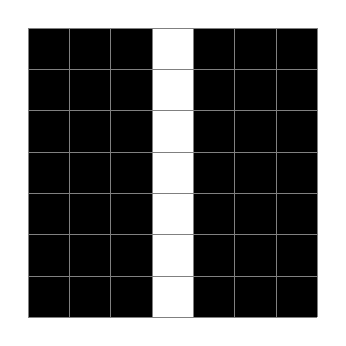
\begin{tikzpicture}[scale=0.525]
	\fill[black] (0,0) rectangle (7,7);
	\fill[white] (3,0) rectangle (4,7);
	\draw[help lines] (0,0) grid (7,7);
	\end{tikzpicture}
	\caption{}\label{10_[7]_In(1)}
\end{subfigure}
\hspace{40pt}
\begin{subfigure}[ht]{0.3\textwidth}
	\centering
	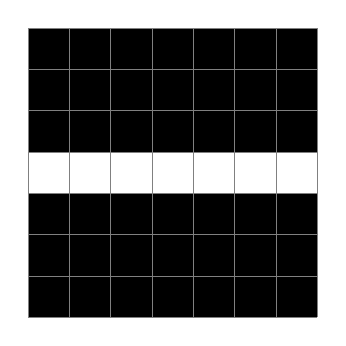
\begin{tikzpicture}[scale=0.525]
	\fill[black] (0,0) rectangle (7,7);
	\fill[white] (0,3) rectangle (7,4);
	\draw[help lines] (0,0) grid (7,7);
	\end{tikzpicture}
        \caption{}\label{10_[7]_In(2)}
\end{subfigure}
\caption{}\label{Filters}
\end{figure}

Now if all neurons in a layer use the same vertical line filter (and the same bias term), and you feed the network the input image shown in Figure~\ref{FeatureMap} (the bottom image), the layer will output the top-left image. Notice that the vertical white lines get enhanced while the rest gets blurred. Similarly, the upper-right image is what you get if all neurons use the same horizontal line filter; notice that the horizontal white lines get enhanced while the rest is blurred out. Thus, a layer full of neurons using the same filter outputs a \emph{feature map}, which highlights the areas in an image that activate the filter the most. Of course, you do not have to define the filters manually: instead, during training the convolutional layer will automatically learn the most useful filters for its task, and the layers above will learn to combine them into more complex patterns.
\begin{figure}[h!t]
\centering
\includegraphics[scale=0.30]{Feature Map}
\caption{}\label{FeatureMap}
\end{figure}
\subsubsection{Stacking multiple feature maps}
Up to now, for simplicity, we have represented the output of each convolutional layer as a 2D layer, but in reality a convolutional layer has multiple filters (you decide how many) and outputs one feature map per filter, so it is more accurately represented in 3D (see Figure~\ref{StackingFeatureMaps}). It has one neuron per pixel in each feature map, and all neurons within a given feature map share the same parameters (i.e., the same weights and bias term). The fact that all neurons in a feature map share the same parameters dramatically reduces the number of parameters in the model, because once the CNN has learned to recognize a pattern in one location, it can recognize it in any other location. Instead, neurons in different feature maps use different parameters. A neuron's receptive field is the same as described earlier, but it extends across all the previous layers' feature maps. In short, a convolutional layer simultaneously applies multiple trainable filters to its inputs, making it capable of detecting multiple features anywhere in its inputs.
\begin{figure}[h!t]
\centering
\includegraphics[scale=0.30]{Stacking Feature Maps}
\caption{}\label{StackingFeatureMaps}
\end{figure}

Input images are also composed of multiple sublayers: one per \emph{color channel}. There are typically three: red, green, and blue (RGB). Grayscale images have just one channel, but some images may have much more—for example, satellite images that capture extra light frequencies (such as infrared).

Specifically, a neuron located in row $i$, column $j$ of the feature map $k$ in a given convolutional layer $l$ is connected to the outputs of the neurons in the previous layer $l-1$, located in rows $i\cdot s_h$ to $i\cdot s_h+f_h-1$ and columns $j\cdot s_w$ to $j\cdot s_w+f_w-1$, across all feature maps (in layer $l-1$). Note that all neurons located in the same row $i$ and column $j$ but in different feature maps are connected to the outputs of the exact same neurons in the previous layer.

All the preceding explanations can be summarized in one big mathematical equation which shows how to compute the output of a given neuron in a convolutional layer:
\begin{equation}
z_{i,j,k}=b_k+\sum_{u=0}^{f_h-1}\sum_{v=0}^{f_w-1}\sum_{k'=0}^{f_{n'}-1}x_{i',j',k'}w_{u,v,k',k}
\end{equation}
with
\begin{equation}
\begin{cases}
i'=i\cdot s_h+u\\
j'=j\cdot s_w+v
\end{cases}
\end{equation}
It is a bit ugly due to all the different indices, but all it does is calculate the weighted sum of all the inputs, plus
the bias term. In this equation:
\begin{itemize}
\item $z_{i,j,k}$ is the output of the neuron located in row $i$, column $j$ in feature map $k$ of the convolutional layer (layer $l$).
\item $b_k$ is the bias term for feature map $k$ (in layer $l$). You can think of it as a knob that tweaks the overall brightness of the feature map $k$.
\item As explained earlier, $s_h$ and $s_w$ are the vertical and horizontal strides, $f_h$ and $f_w$ are the height and width of the receptive field, and $f_{n'}$ is the number of feature maps in the previous layer (layer $l-1$).
\item $x_{i',j',k'}$ is the output of the neuron located in layer $l-1$, row $i'$, column $j'$, feature map $k'$ (or channel $k'$ if the previous layer is the input layer).
\item $w_{u,v,k',k}$ is the connection weight between any neuron in feature map $k$ of the layer $l$ and its input located at row $u$, column $v$ (relative to the neuron's receptive field), and feature map $k'$.
\end{itemize}
Notice that both the weights and the biases do not depend on $i$ and $j$, i.e. on the coordinates of the neuron whose output we are computing.

In summary, it is clear that by introducing convolutional neural networks we have drastically reduced the number of parameters, since every neuron takes the output of only a limited number of neurons of the previous layer. However, this decrease is reflected in the introduction of many more hyperparameters than ``standard'' perceptrons (e.g., width and length of the receptive fields, stride, filters). Therefore we must be more careful to avoid the risk of overfitting.
\subsubsection{Memory requirements}
Another problem with CNNs is that the convolutional layers require a huge amount of RAM. This is especially true during training, because the reverse pass of back-propagation requires all the intermediate values computed during the forward pass.

For example, consider a convolutional layer with $5\times5$ filters, outputting 200 feature maps of size $150\times100$, with stride 1 and eventual padding. If the input is a $150\times100$ RGB image (three channels), then the number of parameters is $(5\times5\times3+1)\times200=\num{15200}$ (the $+1$ corresponds to the bias terms). In fact, all the $150\times100$ neurons within a specific feature map share the same parameters defined by the filter; accordingly each feature map has just $5\times5$ different weights for every input layer, in our case 3. Thus the result is $\num{15200}$, which is fairly small compared to a fully connected layer. However, each of the 200 feature maps contains $150\times100$ neurons, and each of these neurons needs to compute a weighted sum of its $5\times5\times3=75$ inputs: that's a total of 225 million float multiplications. Surely not as bad as a fully connected layer, but still quite computationally intensive. Moreover, if the feature maps are represented using 32-bit floats, then the convolutional layer's output will occupy $200\times150\times100\times32=96$ million bits (\SI{12}{\mega\byte}) of RAM. And that's just for one instance—if a training batch contains 100 instances, then this layer will use up \SI{1.2}{\giga\byte} of RAM!

During inference (i.e., when making a prediction for a new instance) the RAM occupied by one layer can be released as soon as the next layer has been computed, so you only need as much RAM as required by two consecutive layers. But during training everything computed during the forward pass needs to be preserved for the reverse pass, so the amount of RAM needed is (at least) the total amount of RAM required by all layers.

Of course if training crashes because of an out-of-memory error, you can try reducing the mini-batch size. Alternatively, you can try reducing dimensionality using a stride, or removing a few layers. Or you can try using 16-bit floats instead of 32-bit floats.
\subsection{Pooling layers}
Once you understand how convolutional layers work, the \textbf{pooling layers} are quite easy to grasp. Their goal is to subsample (i.e., shrink) the input image in order to reduce the computational load, the memory usage and the number of parameters (thereby limiting the risk of overfitting).

Just like in convolutional layers, each neuron in a pooling layer is connected to the outputs of a limited number of neurons in the previous layer, located within a small rectangular receptive field. You must define its size, the stride, and the padding type, just like before. However, a pooling neuron has no weights; all it does is aggregate the inputs using an aggregation function such as the max or mean.

Figure~\ref{Max_Pooling_Layer} shows a \emph{max pooling layer}, which is the most common type of pooling layer. In this example, we use a $2\times2$ \emph{pooling kernel}, with a stride of 2 and no padding. Only the maximum input value in each receptive field makes it to the next layer, while the other inputs are dropped. For example, in the lower-left receptive field the input values are $1, 5, 3, 2$, so only the maximum value, 5, is propagated to the next layer. Because of the stride of 2, the output image has half the height and half the width of the input image (rounded down since we use no padding).
\begin{figure}[!ht]
\centering
\includegraphics[scale=0.37]{Max Pooling Layer}
\caption{}\label{Max_Pooling_Layer}
\end{figure}

Other than reducing computations, memory usage, and the number of parameters, a max pooling layer also introduces some level of \emph{invariance to small translations}, as shown in Figure~\ref{Invariance_to_Small_Translations}. Here we assume that the bright pixels have a lower value than dark pixels, and we consider three images (A, B, C) going through a max pooling layer with a $2\times2$ kernel and stride 2. Images B and C are the same as image A, but shifted by one and two pixels to the right, respectively. As you can see, the outputs of the max pooling layer for images A and B are identical. This is what translation invariance means. For image C, the output is different: it is shifted one pixel to the right (but there is still \SI{75}{\percent} invariance). By inserting a max pooling layer every few layers in a CNN, it is possible to get some level of translation invariance at a larger scale. Moreover, max pooling offers a small amount of rotational invariance and a slight scale invariance. Such invariance (even if it is limited) can be useful in cases where the prediction should not depend on these details, such as in classification tasks.
\begin{figure}[!ht]
\centering
\includegraphics[scale=0.30]{Invariance to Small Translations}
\caption{}\label{Invariance_to_Small_Translations}
\end{figure}

However, max pooling has some downsides too. Firstly, it is obviously very destructive: even with a tiny $2\times2$ kernel and a stride of 2, the output will be two times smaller in both directions (so its area will be four times smaller), simply dropping \SI{75}{\percent} of the input values. And in some applications, invariance is not desirable. Take semantic segmentation, the task of classifying each pixel in an image according to the object that pixel belongs to: obviously, if the input image is translated by one pixel to the right, the output should also be translated by one pixel to the right. The goal in this case is equivariance, not invariance: a small change to the inputs should lead to a corresponding small change in the output.
%this also happen when we take a photo and we choose to convert the raw image to a smaller resolution
%reduce the complexity
\subsection{Data augmentation}
So far we have seen that convolutional networks (but in general all artificial neural networks) need to perform a huge number of operations during training. Furthermore, the essential element to allow an efficient training is to have a dataset as large as possible, so that the machine learns from as many instances as possible. It is obvious, however, that finding a sufficiently large number of examples is not always easy or possible (for example, taking a million photos of flowers to teach the network to distinguish different species is certainly not practical).

\textbf{Data augmentation} artificially increases the size of the training set by generating many realistic variants of each training instance. This reduces overfitting, making this a regularization technique. The generated instances should be as realistic as possible: ideally, given an image from the augmented training set, a human should not be able to tell whether it was augmented or not. Simply adding white noise will not help; the modifications should be learnable (white noise is not).

For example, you can slightly shift, rotate, and resize every picture in the training set by various amounts and add the resulting pictures to the training set (see Figure~\ref{Data_Augmentation}). This forces the model to be more tolerant to variations in the position, orientation, and size of the objects in the pictures. For a model that's more tolerant of different lighting conditions, you can similarly generate many images with various contrasts. In general, you can also flip the pictures horizontally (except for text, and other asymmetrical objects). By combining these transformations, you can greatly increase the size of your training set.
\begin{figure}[!ht]
\centering
\includegraphics[scale=0.30]{Data Augmentation}
\caption{}\label{Data_Augmentation}
\end{figure}
%tripod vibration?
